\documentclass[11pt,spanish,listoffigures,listoftables]{tfgetsinf}

\usepackage[utf8]{inputenc}
\usepackage{amsmath}
\usepackage{amssymb}
\hypersetup{colorlinks=true, linkcolor=black, urlcolor=cyan}

\graphicspath{{img/}}

\usepackage{booktabs}
\usepackage{array}   % columnas p{} con \raggedright (tablas densas del estado del arte)
\usepackage{tikz}    % esquemas dibujados en el propio texto (Figura del estado del arte)
\usetikzlibrary{babel}   % babel en español activa «>» y rompe las flechas de TikZ sin esto

\usepackage{csquotes}   % biblatex lo exige con babel: comillas de la bibliografía según el idioma
\usepackage[backend=biber,style=numeric,sorting=none]{biblatex}
\addbibresource{references.bib}

% Último recurso de justificación: solo actúa en párrafos que, si no, se saldrían del margen
% (títulos de la bibliografía con compuestos que el silabeado español no parte).
\emergencystretch=1em

% \titulacioname se fija como caption de babel en el .cls (GII) y babel la reaplica en
% \begin{document}; por eso se sobreescribe vía \addto\captionsspanish y no con \renewcommand.
\addto\captionsspanish{\renewcommand{\titulacioname}{Grado en Ciencia de Datos}}

\title{Métricas del gradiente como indicadores de la \\
         eficiencia del entrenamiento en redes neuronales}
\author{Laiqian Ji}
\tutor{Javier Jorge Cano}
\curs{2025-2026}

\date{2026}

\keywords{alineació de gradients, variància del gradient, predicció primerenca, descens per gradient estocàstic, Adam, xarxes neuronals} % valenciano
         {alineación de gradientes, varianza del gradiente, predicción temprana, descenso por gradiente estocástico, Adam, redes neuronales} % castellano
         {gradient alignment, gradient variance, early prediction, stochastic gradient descent, Adam, neural networks}                    % inglés

\begin{document}

% Agradecimientos: página de preliminares, fuera del índice (\chapter* no entra en el TOC).
% Texto pendiente de redacción.
\chapter*{Agradecimientos}

% Resúmenes en valenciano, castellano e inglés.
\begin{abstract}
Entrenar una xarxa neuronal és car, i bona part del còmput es gasta en configuracions que es podien descartar prompte mirant la corba de validació. Els gradients de cada exemple guarden el que eixa corba no veu, la direcció de cada un i la seua dispersió. Este treball pregunta si alguna mètrica calculada sobre eixos gradients en les primeres \emph{epochs} prediu l'eficiència de l'entrenament complet, i si ho fa millor que eixa corba en el mateix moment, sense cost.

L'eficiència es mesura en tres aspectes. La velocitat són les \emph{epochs} que tarda l'\emph{accuracy} de validació a creuar un llindar. El rendiment final és l'\emph{accuracy} de test. La generalització és el \emph{gap}, quant empitjora el \emph{loss} de les dades d'entrenament a les de test. S'han entrenat 960 configuracions, amb quatre conjunts d'imatges (MNIST, CIFAR-10, CIFAR-100 i Tiny-ImageNet), tres arquitectures (una xarxa \emph{fully connected}, una convolucional i una ResNet-18) i dos optimitzadors (SGD i Adam). Cada combinació és una cel·la, i dins d'ella només canvien el \emph{learning rate}, huit valors, i la \emph{seed}, cinc. En cada \emph{epoch} s'han calculat huit mètriques publicades, de dos famílies, alineació i variabilitat, sobre un \emph{batch} fix de 256 exemples.

Dins de cada cel·la, cada mètrica es llig al 5, 10, 25 i 50\,\% del pressupost d'\emph{epochs}. La seua relació amb cada variable d'eficiència es mesura amb la D de Somers, un coeficient de rangs que admet entrenaments que no creuen el llindar, i es compta en quantes de les 24 cel·les eixa relació queda fora del soroll.

Alguna mètrica es relaciona amb l'eficiència. GWA ho fa amb la velocitat en el 67\,\% de les 24 cel·les i amb l'\emph{accuracy} de test en el 63\,\%. Però cap prediu millor que la corba de validació de la mateixa finestra, i eixe és el resultat principal. Triar el \emph{learning rate} amb la millor mètrica perd 2,3 punts d'\emph{accuracy}, i triar-lo amb la validació 1,3. Dins d'una cel·la quasi tot el que canvia és degut al \emph{learning rate}, i les mètriques el reflectixen igual que la validació. Cap família domina, i mesurar al 5\,\% servix tant com al 50\,\%, perquè les mètriques no milloren en esperar. Entre SGD i Adam el sentit canvia com a molt en dos dels 12 parells. De les set prediccions de signe publicades, dos es complixen, tres no troben suport i dos ixen al revés.

En estes condicions, calcular el gradient de cada exemple per a anticipar un entrenament no compensa. Augmenta el cost d'entrenament en una quarta part, i fins al doble en la xarxa \emph{fully connected}. L'estudi conclou que cap de les mètriques estudiades supera la corba de validació com a predictor de l'eficiència, i eixa resposta negativa també és útil, perquè estalvia eixe càlcul a altres. Queden el banc de 960 entrenaments i un mètode per a comparar predictors primerencs amb una referència gratuïta.
\end{abstract}
\begin{abstract}[spanish]
Entrenar una red neuronal es caro, y buena parte del cómputo se gasta en configuraciones que se podían descartar pronto mirando la curva de validación. Los gradientes de cada ejemplo guardan lo que esa curva no ve, la dirección de cada uno y su dispersión. Este trabajo pregunta si alguna métrica calculada sobre esos gradientes en las primeras \emph{epochs} predice la eficiencia del entrenamiento completo, y si lo hace mejor que esa curva en el mismo momento, sin coste.

La eficiencia se mide en tres aspectos. La velocidad son las \emph{epochs} que tarda el \emph{accuracy} de validación en cruzar un umbral. El rendimiento final es el \emph{accuracy} de test. La generalización es el \emph{gap}, cuánto empeora el \emph{loss} de los datos de entrenamiento a los de test. Se han entrenado 960 configuraciones, con cuatro conjuntos de imágenes (MNIST, CIFAR-10, CIFAR-100 y Tiny-ImageNet), tres arquitecturas (una red \emph{fully connected}, una convolucional y una ResNet-18) y dos optimizadores (SGD y Adam). Cada combinación es una celda, y dentro de ella solo cambian el \emph{learning rate}, ocho valores, y la \emph{seed}, cinco. En cada \emph{epoch} se han calculado ocho métricas publicadas, de dos familias, alineación y variabilidad, sobre un \emph{batch} fijo de 256 ejemplos.

Dentro de cada celda, cada métrica se lee al 5, 10, 25 y 50\,\% del presupuesto de \emph{epochs}. Su relación con cada variable de eficiencia se mide con la D de Somers, un coeficiente de rangos que admite entrenamientos que no cruzan el umbral, y se cuenta en cuántas de las 24 celdas esa relación queda fuera del ruido.

Alguna métrica se relaciona con la eficiencia. GWA lo hace con la velocidad en el 67\,\% de las 24 celdas y con el \emph{accuracy} de test en el 63\,\%. Pero ninguna predice mejor que la curva de validación de la misma ventana, y ese es el resultado principal. Elegir el \emph{learning rate} con la mejor métrica pierde 2,3 puntos de \emph{accuracy}, y elegirlo con la validación 1,3. Dentro de una celda casi todo lo que cambia es debido al \emph{learning rate}, y las métricas lo reflejan igual que la validación. Ninguna familia domina, y medir al 5\,\% sirve tanto como al 50\,\%, porque las métricas no mejoran al esperar. Entre SGD y Adam el sentido cambia como mucho en dos de los 12 pares. De las siete predicciones de signo publicadas, dos se cumplen, tres no encuentran apoyo y dos salen al revés.

En estas condiciones, calcular el gradiente de cada ejemplo para anticipar un entrenamiento no compensa. Aumenta el coste de entrenamiento en una cuarta parte, y hasta el doble en la red \emph{fully connected}. El estudio concluye que ninguna de las métricas estudiadas supera a la curva de validación como predictor de la eficiencia, y esa respuesta negativa también es útil, porque ahorra ese cálculo a otros. Quedan el banco de 960 entrenamientos y un método para comparar predictores tempranos con una referencia gratuita.
\end{abstract}
\begin{abstract}[english]
Training a neural network is expensive, and much of the compute goes to configurations that could be discarded early by watching the validation curve. The gradients of individual examples keep what that curve does not see, the direction of each one and their spread. This work asks whether some metric computed on those gradients during the first epochs predicts the efficiency of the full training run, and whether it does so better than that curve at the same moment, at no cost.

Efficiency is measured in three aspects. Speed is the number of epochs the validation accuracy takes to cross a threshold. Final performance is the test accuracy. Generalization is the gap, how much the loss worsens from training data to test data. The study trained 960 configurations, with four image datasets (MNIST, CIFAR-10, CIFAR-100 and Tiny-ImageNet), three architectures (a fully connected network, a convolutional network and a ResNet-18) and two optimizers (SGD and Adam). Each combination is a cell, and within a cell only the learning rate, eight values, and the seed, five, change. At every epoch, eight published metrics, from two families, alignment and variability, were computed on a fixed batch of 256 examples.

Within each cell, each metric is read at 5, 10, 25 and 50\,\% of the epoch budget. Its relation with each efficiency variable is measured with Somers' D, a rank coefficient that admits runs that never cross the threshold, and the number of cells, out of 24, in which that relation stands out from the noise is counted.

Some metric relates to efficiency. GWA does so with speed in 67\,\% of the 24 cells and with test accuracy in 63\,\%. But none predicts better than the validation curve of the same window, and that is the main result. Choosing the learning rate with the best metric loses 2.3 points of accuracy, and choosing it with validation 1.3. Within a cell almost everything that changes is due to the learning rate, and the metrics reflect it just as validation does. No family dominates, and measuring at 5\,\% works as well as at 50\,\%, because the metrics do not improve by waiting. Between SGD and Adam the direction changes in at most two of the 12 pairs. Of the seven published sign predictions, two hold, three find no support and two come out reversed.

Under these conditions, computing the gradient of every example to anticipate a training run does not pay. It raises the training cost by a quarter, and up to twice as much in the fully connected network. The study concludes that none of the metrics studied beats the validation curve as a predictor of efficiency, and that negative answer is also useful, because it saves that computation for others. What remains are the bench of 960 training runs and a method to compare early predictors against a free reference.
\end{abstract}

% La clase genera los índices (general, figuras, tablas) automáticamente al cerrar
% el resumen en inglés; NO llamar a \makeindexes aquí, duplicaría los índices.

% Listado de abreviaturas: tras los índices, fuera del índice (\chapter* no entra en el TOC).
% Revisar al cerrar los capítulos pendientes (resultados, conclusiones, trabajos futuros).
\chapter*{Listado de abreviaturas, siglas y acrónimos}
\begin{description}
  \item[AUC] Área bajo la curva (\textit{area under the curve}).
  \item[CIFAR] Conjuntos de datos CIFAR-10 y CIFAR-100 (\textit{Canadian Institute for Advanced Research}).
  \item[CNN] Red neuronal convolucional (\textit{convolutional neural network}).
  \item[FC] Red totalmente conectada (\textit{fully connected}).
  \item[GNS] Escala de ruido del gradiente (\textit{gradient noise scale}).
  \item[GPU] Unidad de procesamiento gráfico (\textit{graphics processing unit}).
  \item[GSNR] Razón señal-ruido del gradiente por parámetro (\textit{gradient signal-to-noise ratio}).
  \item[GWA] Alineación gradiente-peso (\textit{gradient-weight alignment}).
  \item[MLP] Perceptrón multicapa (\textit{multilayer perceptron}).
  \item[MNIST] Conjunto de datos de dígitos manuscritos (\textit{Modified National Institute of Standards and Technology database}).
  \item[NAS] Búsqueda de arquitecturas neuronales (\textit{neural architecture search}).
  \item[NGV] Varianza normalizada del gradiente (\textit{normalized gradient variance}).
  \item[ODS] Objetivos de Desarrollo Sostenible.
  \item[PAC-Bayes] Marco de cotas de generalización (\textit{probably approximately correct Bayesian}).
  \item[ResNet] Red residual (\textit{residual network}).
  \item[SGD] Descenso por gradiente estocástico (\textit{stochastic gradient descent}).
  \item[TFG] Trabajo de Fin de Grado.
  \item[TSE] Estimador de velocidad de entrenamiento (\textit{training speed estimator}).
\end{description}

\mainmatter

% \includeonly{capitulos/metodologia}  % descomenta para compilar solo un capítulo
\chapter{Introducción}
\label{ch:introduccion}
% Redacción impersonal; sin notas al pie ni referencias en este capítulo (recomendación ETSINF).

En poco más de una década, el aprendizaje automático ha pasado de ser una disciplina de interés sobre todo académico a sostener buena parte de la tecnología de uso cotidiano. Los sistemas que reconocen objetos en imágenes, transcriben voz o generan texto comparten un mismo fundamento, redes neuronales profundas entrenadas sobre grandes volúmenes de datos. Buena parte de los avances del periodo tiene además un origen común, la escala, porque más parámetros, más datos y más tiempo de entrenamiento suelen bastar para mejorar los resultados. La receta funciona y su éxito ha desplazado el cuello de botella de la disciplina. Hoy lo que limita la investigación rara vez son las ideas o los datos. Es el cómputo disponible para ponerlos a prueba.

El coste de esa escala recae primero sobre la industria. Los laboratorios que entrenan los modelos más grandes planifican el trabajo en meses de GPU, con la factura eléctrica que eso supone, y la capacidad de cálculo decide qué organizaciones pueden abordar qué problemas. El coste no es solo económico. El consumo energético del entrenamiento ha hecho de la eficiencia un objeto de estudio, con una línea de trabajo asociada, el llamado \emph{green AI}, que propone valorar los avances también por lo que cuestan.

En la universidad la misma restricción se vive desde el otro lado. Un grupo con menos medios dispone de unas pocas GPU y de un número cerrado de horas de cálculo, y la pregunta pasa de qué modelo entrenar a cómo repartir las horas entre las configuraciones que merezca la pena probar.

Industria y universidad llegan así a la misma pregunta práctica, cuáles de las configuraciones que compiten por las mismas horas merecen seguir y cuánto hay que esperar para saberlo. Esta memoria estudia una de las señales que podrían responderla, los gradientes de la red mientras aprende, y la pone a prueba donde esa decisión se toma, entre entrenamientos de una misma red que solo difieren en el \emph{learning rate}.

Este capítulo presenta el problema que motiva el trabajo y enmarca lo que sigue. La Sección~\ref{sec:motivacion} expone por qué interesa predecir la eficiencia de un entrenamiento desde sus primeras \emph{epochs} y dónde está el hueco que esta memoria pretende cubrir. La Sección~\ref{sec:objetivos} formula la pregunta de investigación y los objetivos que de ella se derivan. La Sección~\ref{sec:alcance} delimita el estudio y separa lo que entra de lo que queda fuera. La Sección~\ref{sec:estructura} cierra el capítulo con un recorrido por el resto de la memoria.

\section{Motivación}
\label{sec:motivacion}

Cada vez que se elige una arquitectura, un optimizador o un conjunto de hiperparámetros, la forma habitual de comprobar si la elección es buena es lanzar el entrenamiento completo y medir el resultado. Se repite muchas veces, porque el espacio de configuraciones posibles es enorme y rara vez se sabe de antemano cuál funcionará mejor.

Buena parte de ese coste se consume en entrenamientos que podrían descartarse pronto. Existen criterios cuantitativos para cortarlos, y todos leen la curva de validación o la de \emph{loss}: extrapolar la curva de aprendizaje desde sus primeras \emph{epochs}, o repartir el presupuesto entre muchas configuraciones y eliminar las peores por rondas, como hace Hyperband. Esas curvas son la señal que ya se mira. La cuestión que plantea este trabajo es si el gradiente contiene información que esas curvas no contienen. Si la contiene, las primeras \emph{epochs} de un presupuesto fijado de antemano bastarían para decidir mejor entre configuraciones y reservar el cómputo para las más prometedoras.

Entre las señales disponibles durante el entrenamiento de una red neuronal, el gradiente es una de las más naturales para observar el progreso del aprendizaje, porque es la información que el optimizador utiliza para avanzar en cada paso. La curva de \emph{loss} resume ese avance en un número por paso. El gradiente de cada ejemplo conserva una estructura que ese promedio descarta, hacia dónde empuja cada ejemplo y cuánto se separan unos de otros. Dos aspectos de esa estructura han recibido atención en trabajos distintos.

El primero es su alineación direccional, esto es, hacia dónde apuntan los gradientes de ejemplos distintos, si al mismo lado o en sentidos opuestos. Es una cuestión de dirección, no de magnitud, que se resume en el ángulo entre ellos. Cuando distintos ejemplos empujan en la misma dirección, sus gradientes se refuerzan y el paso de descenso beneficia a muchos a la vez, mientras que cuando se oponen se cancelan entre sí y el avance se estanca.

El segundo es su variabilidad estocástica. El optimizador ve un \emph{minibatch} cada vez y no todos los datos a la vez, así que el gradiente con el que avanza no es el gradiente verdadero sobre el conjunto completo, sino una estimación a partir de una muestra, y esa estimación cambia según qué ejemplos toquen. La variabilidad mide cuánto se dispersan esos gradientes alrededor de su media, la distancia de cada uno al promedio. Cuando la dispersión es grande, el optimizador recibe estimaciones ruidosas y avanza con dificultad.

En los últimos años se han propuesto varias métricas para cuantificar estos dos aspectos. Cada una se ha presentado en su propio trabajo, con su propio conjunto de datos y su propia arquitectura, y casi siempre con un objetivo distinto, como explicar por qué una red generaliza, elegir el tamaño de \emph{batch} o decidir cuándo detener el entrenamiento. Tres piezas de la pregunta de esta memoria tienen antecedentes. Comparar decenas de medidas sobre un mismo banco de modelos ya se ha hecho para la generalización. Cuán temprano basta medir es la pregunta de la extrapolación de curvas de aprendizaje. Si una medida del gradiente aporta algo sobre una referencia trivial es la pregunta que la búsqueda de arquitecturas se hizo con los \emph{proxies} de coste cero, medidos antes de entrenar, y la respuesta fue muchas veces que no. Lo que sigue sin cubrir es si una métrica del gradiente, medida en las primeras \emph{epochs}, ordena las configuraciones de una misma arquitectura que solo difieren en el \emph{learning rate} mejor que la curva de validación de esas mismas \emph{epochs}, bajo SGD y bajo Adam, y qué cuesta decidir con ella. El Capítulo~\ref{ch:estado-del-arte} sitúa cada antecedente.

Este trabajo cubre ese hueco con un estudio correlacional sistemático. Se entrena una matriz amplia de configuraciones y arquitecturas de redes neuronales para distintos problemas de visión por computador, se calculan en todas ellas las métricas a lo largo del entrenamiento, y se cuantifica en qué medida cada métrica, leída en varias ventanas del proceso, anticipa la eficiencia del entrenamiento completo. El criterio de éxito no es solo que una métrica se asocie con la eficiencia, sino que supere a un predictor de referencia (\emph{baseline}) nombrado de antemano, la curva de validación leída en esa misma ventana, y que no sea esa referencia con otro nombre. El coste de cada métrica se da en su clase de complejidad y en el sobrecoste medido sobre la matriz. Un resultado negativo bien establecido, como por ejemplo la evidencia de que esas métricas no aportan nada que la curva de validación no contenga ya, sería también una contribución útil, porque ahorraría a otros el coste de calcularlas.

\section{Objetivos}
\label{sec:objetivos}

La pregunta de investigación que vertebra la memoria es la siguiente:

\begin{quote}
\itshape ¿Puede alguna métrica del gradiente, medida en las primeras \emph{epochs}, predecir la eficiencia del entrenamiento completo?
\end{quote}

En esta memoria la eficiencia del entrenamiento reúne tres aspectos. La \emph{velocidad de convergencia} es el número de \emph{epochs} que cuesta alcanzar el nivel propio de esa arquitectura en ese problema, leído sobre la curva de validación. El \emph{rendimiento final} es el \emph{accuracy} del modelo sobre el conjunto de test, que se evalúa una sola vez al terminar. La \emph{generalización} es la diferencia entre lo que el modelo logra sobre datos de entrenamiento y sobre datos que no ha visto. Solo el primero es eficiencia en el sentido de rendimiento por unidad de cómputo, y la palabra se usa aquí en ese sentido amplio. Cada aspecto se concreta en una o varias variables en el Capítulo~\ref{ch:metodologia}, y la pregunta se evalúa contra los tres.

La pregunta se responde donde el diseño puede responderla. Con el conjunto de datos, la arquitectura y el optimizador fijos, lo único que cambia entre entrenamientos es el \emph{learning rate} y la \emph{seed}, y toda correlación se calcula dentro de esa celda. Lo que el estudio mide es, por tanto, si una métrica temprana ordena los \emph{learning rates} de una celda mejor que la validación temprana, y cuánto \emph{accuracy} cuesta elegir el \emph{learning rate} con ella. El caso de uso es elegir entre configuraciones, no leer el nivel absoluto de la métrica en un entrenamiento aislado.

El objetivo general del trabajo es cuantificar en qué medida las métricas tempranas de gradiente predicen la eficiencia del entrenamiento completo en tareas de clasificación de imágenes, e identificar cuáles ofrecen la mejor capacidad predictiva y a qué coste. Se concreta en seis objetivos específicos. Los dos primeros son el núcleo del trabajo, y los otros cuatro leen el mismo resultado desde otro ángulo:

\begin{enumerate}
  \item \textbf{OE1 (existencia).} Determinar si al menos una métrica temprana de gradiente se relaciona de forma consistente con la eficiencia en las condiciones estudiadas. Alguna asociación es esperable, porque dentro de una celda el \emph{learning rate} mueve a la vez la métrica y la eficiencia. Por eso este objetivo es un requisito previo de los otros cinco, que sin él carecen de objeto. \label{obj:existencia}
  \item \textbf{OE2 (valor incremental).} Comprobar si alguna métrica supera a una referencia que no cuesta nada, la curva de validación leída en esa misma ventana, sin ser esa referencia con otro nombre. Se decide sobre el rendimiento final y la generalización, porque la velocidad se lee de la misma curva que la referencia. Para el rendimiento se añade una lectura práctica, cuánto \emph{accuracy} se pierde al elegir el \emph{learning rate} con la métrica en vez de con la validación. \label{obj:incremental}
  \item \textbf{OE3 (comparación de familias).} Ordenar las métricas por su capacidad predictiva y ver si las primeras posiciones las ocupa una sola familia. Las dos familias comparten parte de lo que miden, así que la conclusión sobre familias es cualitativa. \label{obj:familias}
  \item \textbf{OE4 (suficiencia temprana).} Determinar cuán temprano basta medir, comparando las ventanas del 5 al 50\,\% del presupuesto. Para la velocidad solo sirven las dos primeras, por una razón que el Capítulo~\ref{ch:metodologia} expone. \label{obj:temprana}
  \item \textbf{OE5 (robustez entre optimizadores).} Evaluar si el sentido de la relación se preserva al cambiar de optimizador, de descenso por gradiente estocástico (SGD) a Adam, comparando cada celda con la que solo difiere en el optimizador. \label{obj:robustez}
  \item \textbf{OE6 (concordancia con la literatura).} Comprobar si el sentido de cada relación observada coincide con el que predice el trabajo que propuso la métrica. Es la lectura con signo de OE1, y solo se contrasta donde el artículo enuncia una predicción; las demás predicciones son extrapolaciones de esta memoria y se reportan sin contrastar. \label{obj:concordancia}
\end{enumerate}

Estos seis objetivos se formalizan en el Capítulo~\ref{ch:metodologia} como las hipótesis H1 a H6, en correspondencia uno a uno con OE1 a OE6, y cada una se enuncia junto al criterio que bastaría para refutarla. El Capítulo~\ref{ch:conclusiones} retoma la lista para examinar, uno a uno, en qué medida se han alcanzado.

\section{Alcance y limitaciones}
\label{sec:alcance}

El trabajo es un estudio \emph{correlacional}. Su finalidad es medir la asociación entre las métricas tempranas y la eficiencia, no intervenir en el entrenamiento a partir de esa señal. El trabajo de diseñar un sistema de intervención, por ejemplo detener el entrenamiento antes de tiempo o ajustar el \emph{learning rate} en función de la alineación medida, queda fuera del alcance y se recoge como línea de trabajo futuro en el Capítulo~\ref{ch:trabajos-futuros}. Como en todo estudio correlacional, las relaciones que se encuentren no deben interpretarse como causales.

El estudio se desarrolla en visión por computador, en concreto en clasificación de imágenes. Abarca cuatro conjuntos de datos de dificultad creciente, tres arquitecturas (una red \emph{fully connected}, una red convolucional simple y una ResNet-18) y dos optimizadores (SGD y Adam). La combinación da lugar a una matriz de experimentos que, con ocho \emph{learning rates} y cinco \emph{seeds} por configuración, suma 960 entrenamientos. El detalle de esta matriz se expone en el Capítulo~\ref{ch:metodologia}.

Dentro de cada celda solo se barre el \emph{learning rate}, con cinco \emph{seeds} por valor. Todo lo demás, del tamaño de \emph{batch} al presupuesto de \emph{epochs}, es idéntico en los 960 entrenamientos y se detalla en el Capítulo~\ref{ch:metodologia}. La configuración de entrenamiento es deliberadamente simple, con \emph{learning rate} constante y sin regularización ni \emph{data augmentation}, y el precio es que los valores de \emph{accuracy} quedan por debajo de los publicados. Las conclusiones valen para esas condiciones.

El método de análisis se fijó después de ejecutar la matriz y antes de calcular ningún coeficiente entre una métrica y una variable de eficiencia, y se revisó después en diez puntos. La Sección~\ref{sec:protocolo-cuando} da las fechas y los motivos.

Quedan fuera del alcance los dominios distintos de la visión, las arquitecturas de tipo \emph{transformer} y los conjuntos de datos a gran escala. El conjunto ImageNet completo se sustituye por una versión reducida, Tiny-ImageNet, por restricciones de disco y de cómputo, y el Capítulo~\ref{ch:metodologia} declara las consecuencias.

\section{Estructura de la memoria}
\label{sec:estructura}

El resto de la memoria se organiza como sigue. El Capítulo~\ref{ch:estado-del-arte} revisa críticamente la literatura, ordenándola en torno a las dos familias de métricas y a los predictores de eficiencia que sirven de referencia, y termina situando la aportación de este trabajo frente a lo existente. El Capítulo~\ref{ch:fundamentos} fija las definiciones formales que el estado del arte deja enunciadas: el descenso por gradiente estocástico, cada una de las métricas y los indicadores de eficiencia. El Capítulo~\ref{ch:metodologia} presenta el diseño experimental: las hipótesis con sus criterios falsables, las variables, la ventana temporal, la configuración del entrenamiento y la matriz de experimentos, la calibración de presupuestos y umbrales, los protocolos de evaluación y de análisis, y los riesgos que el diseño debe neutralizar. El Capítulo~\ref{ch:desarrollo} describe el desarrollo del software que hace posible el estudio. El Capítulo~\ref{ch:resultados} reúne los resultados de los experimentos. El Capítulo~\ref{ch:conclusiones} interpreta esos resultados y revisa el cumplimiento de los objetivos, y el Capítulo~\ref{ch:trabajos-futuros} recoge las líneas de continuación que quedan abiertas. Cierran la memoria los anexos, que recogen la reflexión sobre los Objetivos de Desarrollo Sostenible y los detalles de configuración necesarios para reproducir el estudio.

\chapter{Estado del arte}
\label{ch:estado-del-arte}
% Síntesis crítica de la literatura (qué se hizo y qué se encontró); las fórmulas van en Fundamentos.

Este capítulo revisa la literatura que sostiene el trabajo. No pretende ser exhaustivo, sino selectivo y crítico: de cada propuesta interesa la idea central, lo que sus autores encontraron y, sobre todo, qué deja sin resolver. Las definiciones formales de cada métrica se posponen al Capítulo~\ref{ch:fundamentos}; aquí se manejan en su versión conceptual para no romper el hilo argumental. La Sección~\ref{sec:eda-prediccion} sitúa el problema general de predecir el resultado de un entrenamiento desde sus primeras épocas, un problema que la búsqueda de arquitecturas neuronales lleva años abordando. La Sección~\ref{sec:sota-alineacion} revisa la familia de métricas de alineación o coherencia direccional, y la Sección~\ref{sec:sota-variabilidad} la de variabilidad estocástica. La Sección~\ref{sec:sota-baselines} introduce los predictores que sirven de referencia y que cualquier métrica de gradiente debe superar para justificar su coste. La Sección~\ref{sec:sota-hueco} cierra el capítulo situando la aportación de este trabajo frente a lo revisado.

\section{Predicción temprana de la eficiencia del entrenamiento}
\label{sec:eda-prediccion}

La idea de anticipar el resultado de un entrenamiento sin llegar a completarlo no es nueva. El campo que más la ha trabajado es la búsqueda de arquitecturas neuronales (NAS, por sus siglas en inglés), donde el coste de entrenar a fondo cada arquitectura candidata es prohibitivo: evaluar un espacio de búsqueda completo puede requerir miles de horas de GPU. La respuesta natural ha sido estimar el rendimiento final de cada candidata a partir de unas pocas épocas de entrenamiento, de modo que el ranking aproximado baste para descartar la mayoría y reservar el cómputo para las prometedoras.

El representante más directo de esta línea es el estimador de velocidad de entrenamiento (TSE), propuesto por Ru et al.~\cite{ru2021speedy}. La premisa que lo sustenta es que las arquitecturas que acabarán generalizando mejor tienden a entrenar más deprisa desde el principio, de modo que una suma del loss de entrenamiento temprano, sin tocar el conjunto de test ni un conjunto de validación, ya ordena bien a las candidatas. Los autores muestran que su estimador correlaciona fuertemente, en términos de Spearman y Kendall, con el ranking real de test, y que lo hace de forma más estable que los llamados proxies de coste cero, que se evalúan en la inicialización sin entrenar nada. Su principal ventaja es el coste: el loss de entrenamiento ya se calcula en cada paso, así que el estimador es prácticamente gratuito.

Esa misma ventaja convierte a TSE en el rival a batir, no en un colaborador. Si la curva de loss temprana ya predice el resultado a coste nulo, cualquier métrica que exija instrumentar el gradiente tiene que demostrar que aporta algo por encima de ella. Este trabajo adopta esa exigencia como criterio central, y por eso TSE reaparece como predictor de referencia en la Sección~\ref{sec:sota-baselines}.

\section{Familia de alineación o coherencia direccional}
\label{sec:sota-alineacion}

La primera de las dos grandes familias agrupa las métricas que miden en qué medida los gradientes de ejemplos distintos apuntan hacia el mismo sitio. La intuición compartida es que, cuando ejemplos distintos producen gradientes alineados, la red está aprendiendo características comunes a muchos de ellos en lugar de memorizarlos uno a uno, y que esa coherencia se asocia con un aprendizaje más rápido y una mejor generalización.

El marco conceptual de la familia es la hipótesis de gradientes coherentes de Chatterjee~\cite{chatterjee2020coherent}. Su punto de partida es una descomposición de la norma del gradiente del minibatch en la energía individual de cada ejemplo más los términos cruzados entre pares: cuando los términos cruzados son positivos, el gradiente agregado se refuerza en las direcciones que muchos ejemplos comparten y se cancela en las idiosincráticas, lo que explicaría por qué el descenso por gradiente estocástico generaliza sin sobreajustar de inmediato. El trabajo es sugerente, pero se queda en lo conceptual: sus medidas operativas exigen partir el conjunto de entrenamiento en ejemplos limpios y corruptos mediante ruido de etiquetas controlado, un montaje que no se traslada a un entrenamiento ordinario.

La versión escalable de esa idea es la m-coherencia de Chatterjee y Zielinski~\cite{chatterjee2020making}. Reduce la coherencia a un único escalar calculable sobre un minibatch, con una interpretación intuitiva: aproximadamente el número medio de ejemplos que se benefician del paso de descenso obtenido a partir de un ejemplo cualquiera. Los autores observan, entrenando una ResNet-18 sobre ImageNet~\cite{russakovsky2015imagenet}, que con etiquetas reales la coherencia crece deprisa, mientras que con etiquetas aleatorias también acaba emergiendo, solo que mucho más despacio. De hecho, que la coherencia surja incluso donde no hay estructura que generalizar es el hallazgo que da título al trabajo; lo que separa el aprendizaje de la memorización no es la presencia de coherencia, sino la velocidad con que aparece. La limitación es de cobertura experimental: la evidencia procede de un único conjunto de datos a gran escala, con un tamaño de batch de 4096 y sin data augmentation, condiciones lejanas a las de un entrenamiento típico, y la métrica se estudia como ventana a la memorización, no como predictor de eficiencia.

La stiffness de Fort et al.~\cite{fort2019stiffness} mira el mismo fenómeno con el coseno entre gradientes de pares de ejemplos, pero desagregándolo por clases. Su matriz de stiffness por clase revela jerarquías semánticas que la red descubre sola, por ejemplo, que mejorar la clasificación de gatos ayuda más a la de perros que a la de camiones, y los autores documentan que la stiffness intra-clase decae hacia cero justo cuando empieza el sobreajuste, lo que la señala como indicador temprano. El inconveniente práctico es estadístico: el estimador se basa en promedios sobre pares de un \emph{conjunto de medición} pequeño, y su variante más informativa exige un \emph{conjunto de medición} mayor para no quedar dominada por el ruido muestral, lo que limita su uso como predictor barato en entrenamientos ordinarios.

La gradient confusion de Sankararaman et al.~\cite{sankararaman2020impact} adopta el punto de vista del peor caso: mide el coseno más negativo entre cualquier par de gradientes, es decir, cuán antagónicos llegan a ser los ejemplos. Su aportación más citada es relacionar esta cantidad con la arquitectura: la confusión crece con la profundidad pero decrece con la anchura, lo que ofrece una explicación cuantitativa de por qué la sobreparametrización facilita el entrenamiento. Los autores muestran además que la \emph{batch normalization} y las conexiones residuales la reducen de forma drástica. Como predictor temprano tiene dos debilidades: al ser un estadístico de extremo (un mínimo) es ruidoso, y su cálculo sobre muchos pares es de los más caros de la familia.

La gradient disparity de Forouzesh y Thiran~\cite{forouzesh2021disparity} sustituye el coseno por la distancia entre los gradientes de dos minibatches independientes, y la propone como señal de parada temprana. Es de las pocas métricas de la familia con evidencia cuantitativa fuerte: los autores obtienen, sobre 220 configuraciones, una correlación de Pearson de 0,957 entre las dos versiones de la disparidad, la que compara minibatches de entrenamiento entre sí y la que compara entrenamiento con validación, lo que justifica usar la primera, que no gasta datos de validación, como sustituto de la segunda. Su punto débil es la comparabilidad: la métrica depende del tamaño de batch (su varianza decrece con él), de modo que solo es comparable entre entrenamientos que lo fijen.

La propuesta más reciente de la familia es la alineación gradiente-peso (GWA) de Hölzl~\cite{hoelzl2025gradient}, que mide el coseno entre el gradiente de cada ejemplo y los pesos del clasificador final. Es la métrica con la correlación publicada más alta del corpus revisado: Pearson de 0,99 y Spearman de 0,97 entre su valor máximo a lo largo del entrenamiento y el accuracy de test. Admite además una forma cerrada que la deja casi gratis cuando se calcula solo sobre la última capa. Sus resultados, sin embargo, se obtienen con arquitecturas modernas de tipo convolucional y transformer y con un protocolo orientado a la robustez frente a ruido de etiquetas, por lo que queda abierto si esa correlación tan alta se sostiene en arquitecturas y condiciones distintas.

\section{Familia de variabilidad estocástica}
\label{sec:sota-variabilidad}

La segunda familia no mira la dirección relativa de los gradientes, sino su dispersión. La intuición es complementaria de la anterior: un gradiente cuya estimación varía mucho de un minibatch a otro da al optimizador una señal ruidosa, y la magnitud de ese ruido respecto a la señal condiciona cuánto se puede avanzar por paso y cuál es el tamaño de batch a partir del cual deja de merecer la pena agrandarlo.

El trabajo de referencia es el modelo empírico del entrenamiento con batch grande de McCandlish et al.~\cite{mccandlish2018empirical}, que introduce la escala de ruido del gradiente (GNS): el cociente entre la traza de la covarianza del gradiente y el cuadrado de su norma. Su aportación es predecir el tamaño de batch crítico, el punto a partir del cual duplicar el batch deja de reducir el número de pasos necesarios, sin necesidad de barrer ese hiperparámetro. La métrica es, por construcción, una predicción de un hiperparámetro de entrenamiento más que de la eficiencia final, y su versión exacta requiere la Hessiana; la forma simplificada que se usa en la práctica asume que la curvatura es proporcional a la identidad, una aproximación cómoda pero no inocua.

Faghri et al.~\cite{faghri2020study} estudian directamente la varianza del gradiente y proponen una varianza normalizada que la hace comparable entre problemas de distinta escala. Su hallazgo más llamativo es contraintuitivo: en CIFAR e ImageNet la varianza normalizada crece durante el entrenamiento en lugar de decrecer, lo que contradice la imagen ingenua de que el gradiente se va estabilizando a medida que la red aprende. Es un trabajo descriptivo más que predictivo: mide y caracteriza la varianza, pero no la usa para anticipar la eficiencia de un entrenamiento.

Liu et al.~\cite{liu2020understanding} cierran la familia con la razón señal-ruido del gradiente por parámetro (GSNR), que es esencialmente el inverso de la varianza normalizada. Su tesis es que un GSNR alto durante el entrenamiento se asocia con un menor gap de generalización, y la respaldan con un marco teórico que relaciona el GSNR con la mejora de generalización por paso, y con correlaciones de Pearson de 0,907 a 0,968 entre ambas cantidades. La evidencia, sin embargo, procede en buena parte de entrenamientos con descenso de gradiente puro y tasas de aprendizaje pequeñas, condiciones que aíslan el fenómeno pero se alejan del entrenamiento estocástico habitual.

Conviene situar aquí, como telón de fondo, dos trabajos que no aportan métricas pero justifican el interés por medir la varianza en lugar de combatirla. El gradiente estocástico de varianza reducida de Johnson y Zhang~\cite{johnson2013accelerating} demuestra que reducir explícitamente la varianza del estimador acelera la convergencia bajo convexidad fuerte, lo que legitima la varianza como cantidad relevante para la velocidad de entrenamiento. Pero Defazio y Bottou~\cite{defazio2019ineffectiveness} muestran, de forma empírica, que esa reducción fracasa en redes profundas modernas: la estructura de suma finita sobre la que se apoya se rompe con la batch normalization, el data augmentation y el dropout, hasta el punto de que el método llega a inyectar más varianza de la que elimina. La conclusión que el presente trabajo extrae de ese contraste es que, en aprendizaje profundo real, la varianza del gradiente tiene más valor como señal diagnóstica que como objetivo a minimizar.

Por último, los propios optimizadores del estudio guardan una relación directa con esta familia. El repaso de Ruder~\cite{ruder2016overview} ofrece la taxonomía de variantes de descenso por gradiente, y Adam~\cite{kingma2015adam} y su antecedente RMSProp~\cite{tieleman2012rmsprop} incorporan en su propia mecánica una razón señal-ruido por parámetro: dividen el gradiente por una estimación de su magnitud reciente, que es justamente lo que mide la familia de variabilidad. Esta coincidencia motiva una decisión de diseño que se justifica en el Capítulo~\ref{ch:metodologia}: medir todas las métricas sobre el gradiente bruto, y nunca sobre el paso ya preacondicionado por el optimizador, para que sean comparables entre SGD y Adam.

\section{Predictores de referencia sin instrumentar el gradiente}
\label{sec:sota-baselines}

El valor de este trabajo depende de una comparación honesta. Medir el gradiente cuesta, así que el rival no es la métrica más simple ni la que cada artículo proponga, sino el mejor predictor que se puede obtener sin instrumentar el gradiente en absoluto, leyendo solo lo que el entrenamiento ya produce. Ese predictor de referencia tiene dos componentes, ambos de coste prácticamente nulo.

El primero es el estimador de velocidad de entrenamiento (TSE) de la Sección~\ref{sec:eda-prediccion}, que resume la curva de loss de entrenamiento temprana. El segundo, y probablemente el más fuerte, es la propia métrica de validación medida en la misma fracción temprana del entrenamiento, es decir, el accuracy o el loss de validación a una fracción dada. Es una señal casi gratuita y muy informativa: si las primeras épocas ya separan las configuraciones buenas de las malas en validación, una métrica de gradiente que no supere esa separación no añade nada que merezca su coste.

Estos dos predictores definen el suelo que las métricas de gradiente deben superar. La comparación no se hace solo en términos de correlación cruda, sino de valor incremental: cuánto añade una métrica una vez descontado lo que la curva de loss y la validación temprana ya predicen. Este es el contraste que el objetivo~\ref{obj:incremental} del Capítulo~\ref{ch:introduccion} señala como decisivo, y su formalización se detalla en el Capítulo~\ref{ch:metodologia}.

\section{Posicionamiento de este trabajo}
\label{sec:sota-hueco}

La revisión anterior deja ver un patrón. Cada métrica se ha propuesto y validado por separado, con un objetivo propio (explicar la generalización, elegir el tamaño de batch o decidir cuándo parar), sobre un conjunto de datos y una arquitectura concretos, y rara vez frente al predictor de referencia barato. La Tabla~\ref{tab:sota-metricas} resume las métricas revisadas en los mismos ejes, lo que hace visible esa dispersión: conviven señales de signo y coste muy distintos, evaluadas en bancos de prueba que no se solapan.

Conviene precisar cómo se lee esa tabla. La columna de señal recoge el sentido que cada trabajo asocia con un entrenamiento más eficiente o una mejor generalización, con $\uparrow$ cuando lo deseable es un valor alto y $\downarrow$ cuando lo es un valor bajo. El coste se expresa en relación con el de un paso de entrenamiento y distingue tres tramos: bajo cuando la sobrecarga queda por debajo del cinco por ciento, medio cuando exige un barrido de gradientes por ejemplo sobre el conjunto de medición, y alto cuando además hay que recorrer todos los pares de ese barrido. La columna de evidencia recoge la correlación más fuerte que cada trabajo publica, y es la que pide más cautela, porque las cifras no son comparables entre sí: solo la de GWA relaciona la métrica con el accuracy de test, mientras que la de gradient disparity compara dos variantes de la propia métrica y la de GSNR contrasta los dos lados de la ecuación teórica que sus autores derivan. Los trabajos que respaldan su métrica con figuras y no con un coeficiente aparecen como evidencia cualitativa. Esa heterogeneidad, más que la magnitud de ningún coeficiente concreto, es lo que justifica someter a todas las métricas a una evaluación común.

\begin{table}[ht]
\centering
\footnotesize
\setlength{\tabcolsep}{3pt}
\caption{Síntesis comparativa de las métricas tempranas revisadas.}
\label{tab:sota-metricas}
\begin{tabular}{>{\raggedright\arraybackslash}p{1.9cm}
                >{\raggedright\arraybackslash}p{2.7cm}
                >{\centering\arraybackslash}p{0.9cm}
                >{\raggedright\arraybackslash}p{2.3cm}
                >{\raggedright\arraybackslash}p{2.4cm}
                >{\raggedright\arraybackslash}p{2.3cm}
                >{\centering\arraybackslash}p{1.0cm}}
\toprule
\textbf{Métrica} & \textbf{Qué mide} & \textbf{Señal} & \textbf{Propósito original} & \textbf{Banco de pruebas} & \textbf{Evidencia publicada} & \textbf{Coste} \\
\midrule
\multicolumn{7}{l}{\itshape Familia de alineación o coherencia direccional} \\
\addlinespace[2pt]
m-coherencia \cite{chatterjee2020making} & Ejemplos que se benefician del paso obtenido de uno solo & $\uparrow$ & Separar aprendizaje de memorización & ImageNet; ResNet-18 & Cualitativa & Medio \\
\addlinespace[2pt]
Stiffness \cite{fort2019stiffness} & Coseno entre gradientes de pares, desglosado por clase & $\uparrow$ & Geometría del aprendizaje y aviso de sobreajuste & MNIST, Fashion-MNIST, CIFAR-10/100; MLP, CNN, ResNet-20 & Cualitativa & Medio \\
\addlinespace[2pt]
Gradient confusion \cite{sankararaman2020impact} & Coseno más negativo entre pares, el peor caso & $\downarrow$ & Efecto de la sobreparametrización & CIFAR-10/100, MNIST; redes residuales anchas & Cualitativa & Alto \\
\addlinespace[2pt]
Gradient disparity \cite{forouzesh2021disparity} & Distancia entre los gradientes de dos minibatches & $\downarrow$ & Criterio de parada temprana & MNIST, CIFAR-10/100; AlexNet, VGG-13, ResNet-18 & $r = 0{,}957$ entre sus dos variantes, sobre 220 configuraciones & Bajo \\
\addlinespace[2pt]
GWA \cite{hoelzl2025gradient} & Coseno entre el gradiente y los pesos del clasificador & $\uparrow$ & Proxy de generalización & CIFAR-10/-N/-C, ImageNet-1k/-C; ConvNeXt-F, ViT-S/16 & $r = 0{,}99$ y $\rho = 0{,}97$ frente al accuracy de test & Bajo \\
\addlinespace[3pt]
\multicolumn{7}{l}{\itshape Familia de variabilidad estocástica} \\
\addlinespace[2pt]
Varianza normalizada \cite{faghri2020study} & Varianza del gradiente relativa a su magnitud & $\downarrow$ & Caracterizar la varianza, sin fin predictivo & MNIST, CIFAR-10/100, ImageNet; MLP, ResNet & Cualitativa & Bajo \\
\addlinespace[2pt]
Escala de ruido (GNS) \cite{mccandlish2018empirical} & Traza de la covarianza sobre la norma del gradiente al cuadrado & $\downarrow$ & Predecir el batch size crítico & MNIST, SVHN, CIFAR-10, ImageNet, texto y aprendizaje por refuerzo & Cualitativa & Medio \\
\addlinespace[2pt]
GSNR \cite{liu2020understanding} & Razón señal-ruido del gradiente por parámetro & $\uparrow$ & Explicar la generalización & MNIST, CIFAR-10; CNN, ResNet-18 & $r = 0{,}907$ a $0{,}968$ entre los lados de su ecuación & Medio \\
\addlinespace[3pt]
\multicolumn{7}{l}{\itshape Predictor de referencia, sin instrumentar el gradiente} \\
\addlinespace[2pt]
TSE \cite{ru2021speedy} & Suma del loss de entrenamiento de las primeras épocas & $\downarrow$ & Ordenar arquitecturas en NAS & NAS-Bench-201/301; CIFAR-10/100, ImageNet-16-120 & Spearman y Kendall altos frente al ranking real & Nulo \\
\bottomrule
\end{tabular}
\end{table}

La aportación no es, por tanto, una métrica nueva, sino una evaluación comparativa y rigurosa de las existentes. El resultado que se busca no es coronar a la que mejor predice, sino a la que mejor predice por unidad de coste, lo que se expresa como un frente de Pareto entre potencia predictiva y coste de cómputo. Conviene acotar también lo que el trabajo no puede afirmar: la evidencia se limita a la clasificación de imágenes, con ImageNet sustituido por su versión reducida, y es de naturaleza correlacional, de modo que las relaciones que se encuentren no autorizan conclusiones causales ni una extrapolación automática a otros dominios. El Capítulo~\ref{ch:metodologia} traduce este posicionamiento en un diseño experimental con hipótesis falsables.

\chapter{Fundamentos teóricos}
\label{ch:fundamentos}
% Definiciones formales.

Este capítulo fija las definiciones formales que el Capítulo~\ref{ch:estado-del-arte} maneja en su versión conceptual. La Sección~\ref{sec:notacion} reúne la notación común a modo de glosario de símbolos. Sobre ella se establecen el descenso por gradiente estocástico y la geometría de los gradientes por ejemplo (Secciones~\ref{sec:sgd} y~\ref{sec:geometria}), y a continuación se definen las dos familias de métricas, la de alineación y la de variabilidad (Secciones~\ref{sec:def-alineacion} y~\ref{sec:def-variabilidad}). La Sección~\ref{sec:eficiencia} define los indicadores de eficiencia que actúan como variables a predecir, y la Sección~\ref{sec:fund-conclusiones} recapitula lo establecido. El capítulo define los objetos y, cuando la definición lo exige, anticipa qué agregado concreto se emplea. El protocolo de medición (el \emph{batch} de medición, las ventanas, el suavizado) y las hipótesis con signo asociadas a cada métrica se detallan en el Capítulo~\ref{ch:metodologia}.

\section{Notación}
\label{sec:notacion}

La Tabla~\ref{tab:notacion} recoge los símbolos que se emplean a lo largo de la memoria, con el lugar donde cada uno se introduce y define. Funciona como glosario de consulta. Cada símbolo se define una sola vez, en la sección donde aparece por primera vez, y esta tabla es el punto desde el que localizar esa definición sin releer el capítulo entero.

\begin{table}[!ht]
\centering
\small
\caption{Notación común de la memoria.}
\label{tab:notacion}
\begin{tabular}{cll}
\toprule
\textbf{Símbolo} & \textbf{Significado} & \textbf{Se introduce en} \\
\midrule
$(x_i, y_i)$          & ejemplo de entrenamiento $i$-ésimo                & Sec.~\ref{sec:sgd} \\
$n$                   & número de ejemplos de entrenamiento               & Sec.~\ref{sec:sgd} \\
$f_\theta$            & red neuronal con parámetros $\theta$              & Sec.~\ref{sec:sgd} \\
$P$                   & número de parámetros del modelo                   & Sec.~\ref{sec:sgd} \\
$\ell_i(\theta)$      & \emph{loss} del ejemplo $i$                              & Sec.~\ref{sec:sgd} \\
$\mathcal{L}(\theta)$ & riesgo empírico                                   & Sec.~\ref{sec:sgd} \\
$\eta_t$              & \emph{learning rate} en el paso $t$                & Sec.~\ref{sec:sgd} \\
$B$                   & tamaño del \emph{minibatch}                              & Sec.~\ref{sec:sgd} \\
$\hat{g}$             & gradiente del \emph{minibatch}                           & Sec.~\ref{sec:sgd} \\
$\Sigma$              & covarianza del gradiente por ejemplo              & Sec.~\ref{sec:sgd} \\
$g_i$                 & gradiente por ejemplo                             & Sec.~\ref{sec:geometria} \\
$M$                   & tamaño del \emph{batch} de medición                   & Sec.~\ref{sec:geometria} \\
$\mathbf{G}$          & matriz de Gram de los $g_i$                       & Sec.~\ref{sec:geometria} \\
$s$                   & submuestras disjuntas en la disparidad, $s = 5$ de 51 ejemplos & Sec.~\ref{sec:def-alineacion} \\
$\bar{g}^{(a)}$       & gradiente medio de la submuestra $a$              & Sec.~\ref{sec:def-alineacion} \\
$W$                   & pesos de la última capa lineal                    & Sec.~\ref{sec:def-alineacion} \\
$K$                   & submuestras disjuntas en la NGV, $K = 10$ de 25 ejemplos & Sec.~\ref{sec:def-variabilidad} \\
$\bar{g}$             & gradiente medio del \emph{batch} de medición          & Sec.~\ref{sec:def-variabilidad} \\
$S$, $Q$              & suma de los $g_i$ y suma de sus normas al cuadrado & Sec.~\ref{sec:def-variabilidad} \\
$T$                   & presupuesto de \emph{epochs}                             & Sec.~\ref{sec:eficiencia} \\
$\tau$                & umbral de \emph{accuracy} de validación de la celda      & Sec.~\ref{sec:eficiencia} \\
$t^\star$             & \emph{epochs} hasta el umbral                            & Sec.~\ref{sec:eficiencia} \\
$f$                   & fracción temprana del presupuesto                 & Cap.~\ref{ch:metodologia} \\
\bottomrule
\end{tabular}
\end{table}

% La tabla de notación no cabe en lo que la apertura del capítulo deja libre en la página, ni
% siquiera a cuerpo menor, así que sin este corte LaTeX la empuja dentro de \ref{sec:sgd},
% fuera de la sección que la presenta. El precio son dos páginas más en el total.
\clearpage

\section{Descenso por gradiente estocástico}
\label{sec:sgd}

Sea un conjunto de entrenamiento de $n$ ejemplos $\{(x_i, y_i)\}_{i=1}^n$, una red $f_\theta$ con parámetros $\theta \in \mathbb{R}^P$ y una función de \emph{loss} por ejemplo $\ell_i(\theta) = \ell(f_\theta(x_i), y_i)$. El objetivo del entrenamiento es minimizar el riesgo empírico $\mathcal{L}(\theta) = \tfrac{1}{n}\sum_{i=1}^n \ell_i(\theta)$. El descenso por gradiente estocástico con \emph{minibatch} no evalúa el gradiente exacto $\nabla \mathcal{L}(\theta)$, sino una estimación sobre un subconjunto $I_t$ de $B$ ejemplos extraídos al azar en cada paso:

\begin{equation}
\theta_{t+1} = \theta_t - \eta_t\, \hat{g}_t,
\qquad
\hat{g}_t = \frac{1}{B}\sum_{i \in I_t} \nabla_\theta \ell_i(\theta_t),
\label{eq:sgd}
\end{equation}

donde $\eta_t$ es el \emph{learning rate}. Si el \emph{minibatch} se muestrea de manera uniforme, el estimador es \emph{insesgado}, $\mathbb{E}[\hat{g}_t] = \nabla \mathcal{L}(\theta_t)$, lo que garantiza que SGD optimiza el \emph{loss} correcto y no una distorsión sistemática de él. Su dispersión, en cambio, no es nula. Con ejemplos independientes, la traza de su covarianza vale

\begin{equation}
\operatorname{tr}\operatorname{Cov}[\hat{g}_t] = \frac{\operatorname{tr}(\Sigma)}{B},
\qquad
\Sigma = \operatorname{Cov}_i\!\big[\nabla_\theta \ell_i(\theta_t)\big],
\label{eq:sgd-var}
\end{equation}

con $\Sigma$ la covarianza del gradiente por ejemplo. Esta dispersión escala como $1/B$ pero persiste incluso en el óptimo, donde $\nabla \mathcal{L} = 0$ y aun así $\operatorname{tr}\operatorname{Cov}[\hat{g}] > 0$, porque cada \emph{minibatch} apunta a un objetivo ligeramente distinto. Esa dispersión residual es el suelo de ruido que obliga a reducir progresivamente el \emph{learning rate} para converger, en lugar de orbitar alrededor del mínimo, y es la cantidad que cuantifica la familia de variabilidad.

Los dos optimizadores del estudio parten de ese mismo gradiente y lo transforman de forma distinta. SGD con \emph{momentum} acumula una media móvil de los gradientes y da el paso con ella, y Adam~\cite{kingma2015adam} mantiene dos medias móviles, una del gradiente y otra de su cuadrado por coordenada, y divide la primera por la raíz de la segunda:

\begin{equation}
\text{SGD:}\quad m_t = \mu\, m_{t-1} + \hat{g}_t,\ \ \theta_{t+1} = \theta_t - \eta\, m_t;
\qquad
\text{Adam:}\quad \theta_{t+1} = \theta_t - \eta\, \frac{\hat{m}_t}{\sqrt{\hat{v}_t} + \varepsilon},
\label{eq:momentum-adam}
\end{equation}

donde $\hat{m}_t$ y $\hat{v}_t$ son las dos medias móviles de Adam corregidas por su sesgo inicial. Con $\mu = 0{,}9$ y un gradiente estable, $m_t$ tiende a $\hat{g}/(1 - \mu) = 10\,\hat{g}$, así que el paso efectivo de SGD es unas diez veces el de la Ecuación~\ref{eq:sgd} y sigue siendo proporcional al gradiente. El paso de Adam, al dividir cada coordenada por su propia escala, mide del orden de $\eta$ por coordenada sea cual sea la magnitud del gradiente. Esa diferencia es la razón práctica por la que la rejilla de \emph{learning rates} de Adam se sitúa una década por debajo de la de SGD en la Sección~\ref{sec:matriz}. El argumento no es una igualdad de magnitudes, porque los dos pasos dependen del gradiente de manera distinta; se apoya en los valores por defecto canónicos, $10^{-2}$ para SGD con \emph{momentum} y $10^{-3}$ para Adam, y en una comprobación sobre la matriz: sobre las ocho posiciones de cada rejilla se quedan en el azar 73 entrenamientos con SGD y 81 con Adam, de 480 cada uno, de modo que las dos listas cubren un tramo comparable de su rango útil.

Dos resúmenes estadísticos del gradiente por ejemplo $g$ (que la Sección~\ref{sec:geometria} define formalmente) organizan el resto del capítulo. El \emph{primer momento} $\mathbb{E}[g]$ describe la dirección consistente del gradiente y es lo que estiman el término de inercia (\emph{momentum}) de SGD y la media móvil $m_t$ de Adam~\cite{kingma2015adam}. El \emph{segundo momento}, a través de $\mathbb{E}[\|g\|^2]$ o de la traza de $\Sigma$, describe su magnitud y su dispersión, y es lo que recogen la media móvil $v_t$ de Adam y la escala de ruido del gradiente. Las dos familias de métricas leen, respectivamente, la dirección relativa de los gradientes por ejemplo (alineación) y su dispersión (variabilidad).

Esa lectura fija además una decisión de diseño central del trabajo: todas las métricas se calculan sobre el gradiente bruto $\nabla \ell$ y nunca sobre el paso ya preacondicionado por el optimizador. El motivo es que Adam divide el gradiente por una estimación de su propio segundo momento, que es justamente lo que mide la familia de variabilidad. Medir sobre el paso haría que una misma red, con el mismo gradiente, arrojase valores distintos según el optimizador, y la métrica pasaría a describir en parte la mecánica de este en lugar del aprendizaje. Sobre el gradiente bruto, en cambio, las ocho métricas son la misma cantidad bajo SGD y bajo Adam, que es lo que hace legítima la comparación entre ambos en el Capítulo~\ref{ch:metodologia}.

\section{Geometría del gradiente}
\label{sec:geometria}

El objeto sobre el que se construyen casi todas las métricas es el gradiente por ejemplo

\begin{equation}
g_i = \nabla_\theta\, \ell(f_\theta(x_i), y_i) \in \mathbb{R}^P,
\label{eq:per-sample}
\end{equation}

el gradiente del \emph{loss} de un único ejemplo, antes de promediar. El gradiente del \emph{minibatch} es su media $\hat{g} = \tfrac{1}{B}\sum_i g_i$, pero esa media descarta la estructura estadística que las métricas explotan. La distribución de los $g_i$ (su covarianza, su curtosis) describe el ruido, y sus productos internos por pares describen si los ejemplos cooperan o se cancelan. Para medirlos sin contaminar la dinámica de entrenamiento, todas las métricas se evalúan siempre sobre el mismo \emph{batch} de medición. Se denomina así al subconjunto de $M$ ejemplos, extraído del conjunto de entrenamiento, que se selecciona una única vez al comenzar el entrenamiento y se reutiliza sin cambios en todas las mediciones posteriores. No es una partición de datos adicional junto a las de entrenamiento, validación y test, sino un instrumento de medida. Los ejemplos que lo forman siguen participando en el entrenamiento con normalidad. Se extrae por permutación aleatoria del conjunto de entrenamiento, sin estratificar por clase, así que el número de ejemplos de cada clase que contiene varía con la \emph{seed}. Con $M = 256$ ejemplos y $C$ clases, cabe esperar $\binom{M}{2}/C$ pares de la misma clase: unos 3.264 en MNIST y CIFAR-10, unos 326 en CIFAR-100 y unos 163 en Tiny-ImageNet, de los 32.640 pares posibles. La Sección~\ref{sec:def-alineacion} vuelve sobre ello, porque la \emph{stiffness} intra-clase descansa en esos pares.

Que permanezca fijo es precisamente lo que permite comparar una métrica consigo misma a lo largo del entrenamiento. Si en cada medición se emplearan ejemplos distintos, una variación de la métrica entre dos instantes admitiría dos explicaciones incompatibles, un cambio en el modelo o un remuestreo afortunado, y no habría forma de separarlas. Al congelar los ejemplos, la única fuente de variación que queda es el modelo.

Todas las métricas se calculan con la red en modo de evaluación, esto es, con las capas de \emph{batch normalization} usando las estadísticas acumuladas durante el entrenamiento en lugar de las del lote. En la red \emph{fully connected} y en la convolucional no hay ninguna capa de ese tipo y el modo no cambia nada. En la ResNet-18, la única de las tres que la lleva, es la única forma de definir un gradiente por ejemplo, porque en modo de entrenamiento la salida de cada ejemplo depende del resto del lote. A cambio, el gradiente que se mide es el de la red con sus estadísticas acumuladas, que en las primeras \emph{epochs} no coinciden aún con las del lote, y no exactamente el que desciende el optimizador. Es una diferencia de objeto medido que hay que tener delante al comparar la ResNet-18 con las otras dos arquitecturas.

Las dos operaciones elementales son la matriz de Gram y la similitud coseno. La matriz de Gram recoge todos los productos internos por pares, $\mathbf{G}_{ij} = \langle g_i, g_j\rangle$, y la similitud coseno los normaliza por magnitud:

\begin{equation}
\cos(g_i, g_j) = \frac{\langle g_i, g_j\rangle}{\|g_i\|\,\|g_j\|} \in [-1, 1].
\label{eq:cosine}
\end{equation}

El coseno vale $1$ si los dos gradientes apuntan en la misma dirección, $0$ si son ortogonales y $-1$ si son opuestos. La normalización por norma importa porque lo relevante para la cooperación entre ejemplos es la dirección relativa, no la escala individual de cada gradiente.

Conviene detenerse en un hecho de alta dimensión, porque fija la escala con la que hay que leer cualquier coseno entre gradientes. Se llama \emph{isótropo} a un vector aleatorio cuya distribución no privilegia ninguna dirección del espacio, esto es, que es invariante frente a rotaciones. El caso canónico es un vector gaussiano con covarianza proporcional a la identidad o, lo que es lo mismo una vez normalizado, un punto uniforme sobre la esfera unidad. Si $u$ y $v$ son dos vectores isótropos independientes en $\mathbb{R}^P$, su coseno tiene media nula y varianza exactamente $1/P$, de modo que su magnitud típica es del orden de $1/\sqrt{P}$. No se trata solo de que la media sea cero. La distribución se concentra exponencialmente en torno a ese valor, con $\Pr[\,|\cos(u,v)| \ge t\,]$ decayendo como $\exp(-P t^2 / 2)$, que es el fenómeno de concentración de la medida sobre la esfera~\cite{vershynin2018high}. Dicho de otro modo, en dimensión alta dos direcciones tomadas al azar son casi ortogonales, y lo son tanto más cuanto mayor es $P$~\cite{blum2020foundations}.

Ese cálculo fija la escala del ruido de muestreo, no la referencia contra la que leer una métrica. En los modelos de este trabajo $P$ va desde unos $1{,}9 \times 10^{4}$ parámetros en la CNN pequeña hasta más de $10^{7}$ en ResNet-18 y en la red \emph{fully connected} sobre Tiny-ImageNet, lo que sitúa el coseno entre dos direcciones sin relación alguna entre $7 \times 10^{-3}$ y $3 \times 10^{-4}$. Los gradientes por ejemplo de una red no son direcciones sin relación, ni siquiera en la inicialización. Con entropía cruzada, el gradiente respecto a la última capa es $(p - y)\,z^\top$, donde $p$ son las probabilidades predichas, $y$ la etiqueta en codificación \emph{one-hot} y $z$ la entrada de esa capa. Dos ejemplos de la misma clase comparten el signo del factor $(p - y)$ y, con activaciones ReLU no negativas, sus gradientes forman un ángulo agudo antes de haber aprendido nada, mientras que dos ejemplos de clases distintas tienden a oponerse. La \emph{stiffness} intra-clase es positiva y la inter-clase negativa por estructura, y la referencia honesta de cada métrica de alineación es su valor en la inicialización. La matriz no lo registra, porque la primera medición se hace al final de la primera \emph{epoch}. Los valores registrados muestran esa estructura: sobre las 33.600 filas de la matriz, el coseno medio entre todos los pares del \emph{batch} de medición tiene mediana $0{,}0019$ en la CNN, $0{,}0005$ en la red \emph{fully connected} y $0{,}009$ en la ResNet-18, es decir, en el suelo del ruido en las dos primeras y unas treinta veces por encima en la tercera, mientras que el coseno entre pares de la misma clase tiene mediana entre $0{,}30$ y $0{,}51$ en las tres y el de pares de clases distintas se queda en cero. Lo que garantiza el argumento de concentración es que una desviación como esa es un hecho de la red y no una fluctuación del muestreo. El argumento alcanza también a los estadísticos de extremo. Al recorrer los $\binom{M}{2}$ pares del \emph{batch} de medición, el coseno más negativo esperable entre direcciones sin relación solo alcanza en magnitud el orden de $\sqrt{\log M / P}$, de manera que tampoco un valor apreciable de \emph{gradient confusion} puede atribuirse al azar del muestreo.

\section{Métricas de alineación}
\label{sec:def-alineacion}

La familia de alineación cuantifica en qué medida los gradientes de ejemplos distintos apuntan hacia el mismo sitio. Su marco conceptual es la descomposición de la norma del gradiente del \emph{minibatch}~\cite{chatterjee2020coherent},

\begin{equation}
\Big\|\sum_i g_i\Big\|^2 = \sum_i \|g_i\|^2 + \sum_{i \neq j} \langle g_i, g_j\rangle,
\label{eq:cgh}
\end{equation}

donde el primer término suma el tamaño al cuadrado del gradiente de cada ejemplo, esto es, lo que cada uno aporta por su cuenta, y el segundo suma el producto interno de cada par de gradientes distintos, positivo cuando los dos apuntan al mismo lado y negativo cuando se oponen. En ese segundo término vive la coherencia, y las métricas siguientes son distintos agregadores de él.

\paragraph{m-coherencia.} Reduce la coherencia a un único escalar sobre el \emph{batch} de medición de $M$
ejemplos~\cite{chatterjee2020making}:

\begin{equation}
\alpha = \frac{\big\|\sum_{i=1}^{M} g_i\big\|^2}{\sum_{i=1}^{M} \|g_i\|^2} \in [0, M].
\label{eq:mcoherence}
\end{equation}

Vale $M$ cuando los gradientes son idénticos, en dirección y en norma, y $1$ en el \emph{límite ortogonal}, donde son mutuamente perpendiculares, cualquiera que sea su norma. Por debajo de $1$ los gradientes están anticorrelados. Su lectura intuitiva es el número medio de ejemplos que se benefician de un paso de descenso obtenido a partir del gradiente de un ejemplo cualquiera. Una alineación mayor se asocia con un aprendizaje más coherente, de modo que se espera que una $\alpha$ alta acompañe a un entrenamiento eficiente.

\paragraph{Stiffness.} Mide el coseno entre gradientes de pares de ejemplos, desagregado
por clases~\cite{fort2019stiffness}. Sobre el \emph{batch} de medición se definen una variante de coseno y una de signo,

\begin{equation}
S_{\cos} = \mathbb{E}_{i \neq j}\!\big[\cos(g_i, g_j)\big],
\qquad
S_{\operatorname{sign}} = \mathbb{E}_{i \neq j}\!\big[\operatorname{sign}\langle g_i, g_j\rangle\big],
\label{eq:stiffness}
\end{equation}

cada una restringida a pares de la misma clase ($y_i = y_j$, \emph{stiffness} \emph{intra-clase}) o de clases distintas ($y_i \neq y_j$, \emph{inter-clase}). Una \emph{stiffness} intra-clase alta indica que la red ha aprendido características compartidas y que cada paso de gradiente sobre un ejemplo beneficia al resto de su clase. La columna que representa a la métrica es el coseno intra-clase, según fija la Sección~\ref{sec:variables}, y la media se toma sobre todos los pares mezclados, no como media de una matriz por clases como en el artículo. Con el \emph{batch} de medición sin estratificar de la Sección~\ref{sec:geometria}, ese coseno descansa en unos 163 pares en Tiny-ImageNet y unos 326 en CIFAR-100, y su composición cambia con la \emph{seed}. Fort et al. afirman que la señal predictiva es más fuerte en la fase temprana, porque la \emph{stiffness} decae hacia cero cuando comienza el sobreajuste; es una afirmación del artículo y no un hecho medido aquí.

\paragraph{Gradient confusion.} Adopta el punto de vista del peor caso y toma el coseno más
negativo entre cualquier par de gradientes del \emph{batch} de medición~\cite{sankararaman2020impact}. En su forma normalizada,

\begin{equation}
\hat{\eta} = -\min_{i \neq j} \cos(g_i, g_j).
\label{eq:confusion}
\end{equation}

Un $\hat{\eta}$ alto señala que existe al menos un par de ejemplos cuyos gradientes se oponen con fuerza, lo que frena el avance neto de SGD. Un $\hat{\eta}$ cercano a cero indica gradientes que no se contradicen. Por ser un estadístico de extremo es ruidoso, así que junto al mínimo se registran estadísticos de la distribución de cosenos: su mediana, su percentil 5 y la fracción de pares negativos. El artículo de origen la estima sobre 100 pares de gradientes de \emph{minibatch} de 128 ejemplos al final de cada \emph{epoch}. Aquí es el mínimo sobre los 32.640 pares de gradientes por ejemplo del \emph{batch} de medición, un extremo sobre muchos más pares y de otra distribución, así que su magnitud no es comparable con las cifras del artículo, aunque su orden dentro de una celda sí lo es. La columna titular se mantiene en el mínimo por fidelidad a la definición original. Se predice que una confusión menor acompaña a un entrenamiento más rápido.

\paragraph{Gradient disparity.} Sustituye el coseno por la distancia entre los gradientes
medios de dos submuestras independientes, derivada de una cota de tipo PAC-Bayes~\cite{forouzesh2021disparity}. Si el \emph{batch} de medición se parte en $s$ submuestras disjuntas y $\bar{g}^{(a)}$ denota el gradiente medio de la submuestra $a$,

\begin{equation}
\overline{\mathcal{D}} = \binom{s}{2}^{-1} \sum_{a < b} \big\|\bar{g}^{(a)} - \bar{g}^{(b)}\big\|_2.
\label{eq:disparity}
\end{equation}

Es una magnitud $\ell_2$ \emph{sin normalizar}, no una similitud coseno, porque la cota teórica del trabajo depende de $\|\bar{g}^{(a)} - \bar{g}^{(b)}\|_2^2$ y dividir por la norma rompería la conexión con la teoría. Aquí $s = 5$ y cada submuestra tiene 51 ejemplos. Esa forma tiene una consecuencia que la definición no deja ver. Si las submuestras son disjuntas y de tamaño $b$, la esperanza de $\|\bar{g}^{(a)} - \bar{g}^{(b)}\|^2$ es $2\operatorname{tr}(\Sigma)/b$, y en dimensión alta la norma se concentra en su esperanza, así que la disparidad es, salvo el ruido de muestreo, la raíz de $2\operatorname{tr}(\Sigma)/51$: la dispersión del gradiente por ejemplo sin normalizar por la señal. Sobre las 33.600 filas de la matriz, el cociente entre el cuadrado de la disparidad y la traza de la covarianza tiene mediana $0{,}038$, con la mitad central entre $0{,}036$ y $0{,}040$, frente al $2/51 = 0{,}039$ del álgebra, y su correlación de Spearman con esa traza dentro de un mismo entrenamiento tiene mediana $0{,}99$. Por eso, desde el 3 de septiembre de 2026, esta métrica cuenta en la familia de variabilidad y no en la de alineación, como recoge la Sección~\ref{sec:protocolo-objetivos}. Es además la única de las ocho que no es invariante a la escala del gradiente, de modo que dentro de una celda recoge en parte cuánto mide el gradiente en ese momento. Una disparidad baja indica submuestras coherentes, y se predice como señal de eficiencia, con la salvedad de que su magnitud depende del tamaño de la submuestra, 51 aquí, y solo es comparable entre entrenamientos que lo fijen.

\paragraph{Alineación gradiente-peso (GWA).} Mide el coseno entre el gradiente por ejemplo
y los pesos de la última capa lineal de la red, la que convierte la representación aprendida en una puntuación por clase, con el gradiente restringido también a esa capa~\cite{hoelzl2025gradient}. Con $W$ los pesos de esa capa, sin el sesgo, y $g_i^{(W)}$ el gradiente de $\ell_i$ respecto a ellos, para cada ejemplo del \emph{batch} de medición se toma $\gamma_i = \cos\!\big(g_i^{(W)}, W\big)$, y el agregado por \emph{epoch} corrige la media por el exceso de curtosis de la distribución de los $\gamma_i$:

\begin{equation}
\mathrm{GWA} = \frac{\bar{\gamma}}{\dfrac{\mu_4}{\mu_2^{2}} - 3 + \beta},
\qquad \beta = 1{,}2,
\label{eq:gwa}
\end{equation}

donde $\bar{\gamma}$ es la media de las $\gamma_i$, $\mu_2$ y $\mu_4$ sus momentos centrales de segundo y cuarto orden, y $\mu_4/\mu_2^2 - 3$ el exceso de curtosis (nulo para una gaussiana). El denominador descuenta las distribuciones de cola pesada, donde pocas muestras dominan la media.

Cada $\gamma_i$ tiene una lectura directa en términos de la red. Con entropía cruzada y logits $Wz + b$, el producto interno entre el gradiente de $W$ y la propia $W$ vale $\sum_c (p_c - y_c)\,(Wz)_c$, la diferencia entre el logit medio bajo las probabilidades predichas y el logit de la clase correcta, y $\gamma_i$ es esa cantidad dividida por las dos normas. Cuanto más domina el logit de la clase correcta, más negativo es $\gamma_i$. GWA es, por tanto, un margen normalizado medio de la red sobre los 256 ejemplos del \emph{batch} de medición, corregido por la forma de su distribución. Eso explica que en su artículo siga tan de cerca al \emph{accuracy} de test, porque es una cantidad que el propio paso hacia delante casi regala, y anticipa que dentro de una celda irá muy cerca del \emph{accuracy} de validación leído en la misma ventana. Los valores registrados lo confirman en el rango: la media $\bar{\gamma}$ vive entre $-0{,}18$ y $0{,}02$ en toda la matriz. El cociente de la Ecuación~\ref{eq:gwa}, en cambio, recorre de $-63$ a $131$, porque el denominador se hace negativo cuando el exceso de curtosis baja de $-1{,}2$, cosa que ocurre en el 1,8\,\% de las filas registradas y en ninguna de la ventana del 5\,\% que lee el análisis primario. En esas filas GWA cambia de signo sin que la media lo haga, y las ventanas exploratorias se leen con ese aviso. Hay además una salvedad de signo que condiciona toda lectura posterior de esta métrica. El trabajo de origen define el gradiente como $-\nabla\ell$ y concluye que una GWA \emph{alta} se asocia con mejor generalización. Como aquí se mide sobre el gradiente bruto $\nabla\ell$, por la decisión de la Sección~\ref{sec:sgd}, el signo queda invertido respecto al original. La predicción heredada, expresada en la convención de esta memoria, es que una GWA \emph{baja} acompañe a una mejor generalización. El Capítulo~\ref{ch:metodologia} contrasta el signo observado contra esta forma ya convertida, y no contra la del artículo.

Cada una de estas definiciones lleva implícita una predicción direccional: más coherencia, más \emph{stiffness} intra-clase, menos confusión y menos disparidad deberían acompañar a un entrenamiento más eficiente, y, con la salvedad de signo que se acaba de describir, una GWA más baja a una mejor generalización. Esas predicciones con signo se formalizan como hipótesis falsables en el Capítulo~\ref{ch:metodologia}.

\section{Métricas de variabilidad}
\label{sec:def-variabilidad}

La familia de variabilidad no mira la dirección relativa de los gradientes, sino su dispersión respecto a la señal. Sus tres métricas, y desde el 3 de septiembre de 2026 también la \emph{gradient disparity}, son facetas de una misma cantidad, la dispersión del gradiente por ejemplo medida contra su media.

\paragraph{Varianza normalizada (NGV).} Hace comparable la varianza del gradiente entre
problemas de distinta escala dividiéndola por la magnitud de la señal~\cite{faghri2020study}. Se estima sobre $K = 10$ submuestras disjuntas de 25 ejemplos del \emph{batch} de medición, cuyos gradientes medios aportan las $K$ observaciones sobre las que se toman la esperanza y la covarianza:

\begin{equation}
\mathrm{NGV} = \frac{\operatorname{tr}\!\big(\operatorname{Cov}(g)\big)}{\|\mathbb{E}[g]\|^2}.
\label{eq:ngv}
\end{equation}

Es el inverso de una razón señal-ruido. Por debajo de $1$ la señal del gradiente medio domina sobre el ruido, y por encima domina el ruido. Esta forma, de tipo traza sobre norma, es una adaptación deliberada de la versión literal del trabajo de origen ($\mathbb{V}[g_j]/\mathbb{E}[g_j^2]$ por coordenada), monótonamente equivalente. Una NGV menor indica menos ruido relativo, si bien empíricamente la métrica crece durante el entrenamiento en lugar de decrecer. La razón es elemental. Sin regularización, a medida que la red ajusta los ejemplos del \emph{batch} de medición el gradiente medio tiende a cero mientras la dispersión entre ejemplos no, así que el cociente sube. Dentro de una celda, el \emph{learning rate} decide cuánto ha avanzado la red cuando se mide, luego estas columnas son en buena parte cuánto ha bajado ya el \emph{loss}, leído con otra regla; es el mecanismo de la causa común que el Capítulo~\ref{ch:resultados} mide. El estimador tiene además un techo. El denominador se estima con la norma del gradiente medio de las $K$ submuestras, que está sesgada hacia arriba por $\operatorname{tr}(\Sigma)/K$, y por eso la NGV registrada no puede pasar de $K = 10$ aunque la señal sea nula; su mediana sobre la matriz es $8{,}1$, pegada a ese techo. Desde el 3 de septiembre de 2026 la NGV no entra en el contraste, porque es la escala de ruido de la Ecuación~\ref{eq:gns} estimada con diez submuestras en lugar de con los 256 ejemplos, y la escala de ruido la representa (Sección~\ref{sec:protocolo-objetivos}).

\paragraph{Escala de ruido del gradiente (GNS).} Predice el tamaño de \emph{batch} crítico, aquel
a partir del cual ampliar el \emph{batch} deja de reducir el número de pasos, sin necesidad de barrer ese hiperparámetro~\cite{mccandlish2018empirical}. Su forma simplificada es

\begin{equation}
\mathcal{B}_{\text{simple}} = \frac{\operatorname{tr}(\Sigma)}{\|\bar{g}\|^2},
\label{eq:gns}
\end{equation}

con $\Sigma$ la covarianza por ejemplo y $\bar{g}$ el gradiente medio. La versión exacta $\mathcal{B}_{\text{noise}} = \operatorname{tr}(H\Sigma)/(\bar{g}^\top H \bar{g})$ requiere la Hessiana $H$ y se descarta por coste. La simplificada asume $H \propto I$. Por construcción, $\mathcal{B}_{\text{simple}} \approx 25 \cdot \mathrm{NGV}$, donde 25 es el tamaño de las submuestras con las que se estima la NGV y no el tamaño de \emph{batch} del entrenamiento; la relación es exacta para las cantidades poblacionales y solo aproximada para los estimadores.

Estimada sobre el \emph{batch} de medición con gradientes por ejemplo, la escala de ruido guarda además una relación que no es aproximada sino una identidad algebraica, y que cruza la frontera entre las dos familias. Con $S = \sum_i g_i$ y $Q = \sum_i \|g_i\|^2$ se tiene $\|\bar{g}\|^2 = \|S\|^2/M^2$ y $\operatorname{tr}(\Sigma) = Q/M - \|S\|^2/M^2$, de donde

\begin{equation}
\mathcal{B}_{\text{simple}} = \frac{M}{\alpha} - 1,
\label{eq:gns-mcoh}
\end{equation}

con $\alpha$ la m-coherencia de la Ecuación~\ref{eq:mcoherence}. Ambas dependen solo del cociente $\|S\|^2/Q$, de modo que son la misma cantidad reparametrizada y su correlación de Spearman dentro de un mismo entrenamiento está forzada a $-1$ exacto. El piloto de calibración lo verificó a un error relativo de $8{,}8 \times 10^{-6}$, atribuible al redondeo en coma flotante. La consecuencia es que la escala de ruido y la m-coherencia no aportan evidencia independiente pese a pertenecer a familias distintas, y la NGV tampoco, porque es esta misma razón estimada con diez submuestras. Las tres son estimadores de $\alpha$, la razón entre $\|S\|^2$ y $Q$; solo GSNR agrega de otra manera, por coordenada. Desde el 3 de septiembre de 2026 la m-coherencia y la NGV salen del contraste y la escala de ruido las representa, como recoge la Sección~\ref{sec:protocolo-objetivos}, y la predicción de signo del artículo de la m-coherencia se lee sobre la escala de ruido con el signo cambiado, porque la Ecuación~\ref{eq:gns-mcoh} es decreciente en $\alpha$.

El estimador de la escala de ruido tiene un techo, y está cerca de él. Si el gradiente medio verdadero es cero, $\mathbb{E}\|S\|^2 = Q$, $\alpha$ tiende a $1$ y la escala de ruido estimada a $M - 1 = 255$. McCandlish et al. reportan escalas de $10^{3}$ a $10^{4}$ en CIFAR-10 e ImageNet, muy por encima de lo que 256 ejemplos pueden resolver, así que el estimador vive pegado a su techo: sobre las 33.600 filas de la matriz la mediana es $207$, el percentil 5 es $58$ y el percentil 95 es $287$, con la mitad de las filas por encima de $204$. Las magnitudes registradas no se pueden leer, por tanto, como el tamaño de \emph{batch} crítico que la métrica promete, y la transformación $M/\alpha - 1$ amplifica cerca de $\alpha = 1$ cualquier fluctuación de $\alpha$. Lo que sí conserva sentido es el orden entre entrenamientos de una misma celda, que es lo que el análisis usa, con menos potencia de la que tendría un estimador lejos de su techo. McCandlish et al. dan un estimador sin sesgo de la señal, $\|\bar{g}\|^2 - \operatorname{tr}(\hat{\Sigma})/M$, que puede salir negativo y declarar entonces que la señal no es detectable con 256 ejemplos; se puede calcular desde las columnas registradas y no se calculó.

\paragraph{Razón señal-ruido del gradiente por parámetro (GSNR).} Lleva la razón señal-ruido al nivel de
cada parámetro $\theta_j$~\cite{liu2020understanding}:

\begin{equation}
r(\theta_j) = \frac{\tilde{g}(\theta_j)^2}{\sigma^2(\theta_j)},
\qquad
\tilde{g}(\theta_j) = \mathbb{E}_i[g_{i,j}],
\quad
\sigma^2(\theta_j) = \operatorname{Var}_i[g_{i,j}],
\label{eq:gsnr}
\end{equation}

agregado por la media sobre los parámetros, nunca por la suma, que sería incomparable entre arquitecturas de distinto tamaño. El estimador usa la varianza insesgada sobre los $M$ ejemplos, descarta los parámetros cuyo gradiente es nulo en todo el \emph{batch} de medición, y bajo señal nula tiene un suelo de $1/M \approx 0{,}004$ por parámetro, porque el cuadrado de la media de $M$ valores de ruido vale en esperanza su varianza dividida por $M$. La media sobre millones de parámetros la domina la cola pesada de $r(\theta_j)$, y por eso se registran también la mediana y el percentil 95; la columna titular es la media por fidelidad a Liu et al. Es esencialmente el recíproco por parámetro de la NGV. Un GSNR alto significa que la media del gradiente por ejemplo domina a su varianza, y se asocia con un \emph{gap} de generalización pequeño. Las tres métricas miden, pues, la misma razón señal-ruido desde ángulos distintos. La redundancia entre ellas es algebraica y se resuelve por álgebra antes del contraste, como recoge la Sección~\ref{sec:protocolo-objetivos}: queda la escala de ruido como representante de $\alpha$, y GSNR aparte porque agrega por coordenada.

\section{Indicadores de eficiencia del entrenamiento}
\label{sec:eficiencia}

Las métricas anteriores son las variables predictoras. Las que siguen son las variables a predecir, esto es, lo que en este trabajo se entiende por eficiencia del entrenamiento. Se leen sobre la curva de validación a lo largo del presupuesto de \emph{epochs} $T$. El protocolo concreto, incluido el suavizado de la curva, la separación entrenamiento/validación/test y el tratamiento del censurado en el análisis, se especifica en el Capítulo~\ref{ch:metodologia}.

\paragraph{Epochs hasta el umbral (indicador primario).} El número de \emph{epochs} que tarda la
\emph{accuracy} de validación en alcanzar un nivel objetivo $\tau$ propio de cada conjunto de datos y arquitectura,

\begin{equation}
t^\star = \min\{\, t \le T : \mathrm{acc}_{\text{val}}(t) \ge \tau \,\}.
\label{eq:epochs-to-threshold}
\end{equation}

Si el \emph{accuracy} no cruza el umbral dentro del presupuesto, el valor queda \emph{censurado} y se anota como ausente, nunca como el valor del presupuesto. Los extremos de la rejilla de \emph{learning rates} no alcanzan el umbral por diseño. Descartar un entrenamiento lento pero vivo sesgaría la muestra, y por eso se conserva como censurado; distinto es un entrenamiento que nunca aprendió, que no es lento sino que está muerto, y la Sección~\ref{sec:protocolo-poblacion} lo deja fuera de la población con ese criterio. Un $t^\star$ menor indica un entrenamiento más rápido.

\paragraph{AUC del \emph{loss} de validación.} El área bajo la curva de \emph{loss} de validación
dentro del presupuesto, aproximada por la regla trapezoidal sobre el eje de \emph{epochs}. Resume toda la trayectoria en un escalar. Cuanto menor es el área, más rápido y más bajo desciende el \emph{loss}, siempre que la curva descienda. En el régimen de este estudio, sin \emph{weight decay} ni \emph{data augmentation}, el \emph{loss} de validación toca fondo pronto y vuelve a subir, y el área recoge entonces sobre todo esa subida: en las celdas de la red \emph{fully connected} y de la ResNet-18 fuera de MNIST el mínimo llega entre la \emph{epoch} 4 y la 8 de mediana, y entre el 84 y el 94\,\% del área queda después de él. Ahí el área ordena los entrenamientos por cuánto sobreajustan más que por lo rápido que aprenden, y así se lee.

\paragraph{Mejor \emph{loss} de validación.} El mínimo del \emph{loss} de validación alcanzado
dentro del presupuesto, que mide el mejor nivel intermedio con independencia de la velocidad con que se alcanza. Es una variable de nivel, y desde el 3 de septiembre de 2026 se lee como apoyo del rendimiento final y no de la velocidad, según fija la Sección~\ref{sec:variables}.

\paragraph{Rendimiento final.} El \emph{accuracy} sobre el conjunto de test, evaluado una única
vez al terminar el entrenamiento. Es la variable objetivo certificada, separada de la curva de validación que se monitoriza durante el entrenamiento.

\paragraph{Gap de generalización.} La diferencia final entre el rendimiento en test y en
entrenamiento, medida sobre un subconjunto fijo del conjunto de entrenamiento del mismo tamaño que el de test. En términos de \emph{loss} y de \emph{accuracy},

\begin{equation}
\mathrm{gap}_{\text{loss}} = \mathcal{L}_{\text{test}} - \mathcal{L}_{\text{train}},
\qquad
\mathrm{gap}_{\text{acc}} = \mathrm{acc}_{\text{train}} - \mathrm{acc}_{\text{test}},
\label{eq:gap}
\end{equation}

donde un valor positivo indica sobreajuste. Es la variable objetivo de generalización frente a la que se contrastan, en particular, las métricas que sus trabajos de origen vinculan a este \emph{gap}.

\section{Conclusiones del capítulo}
\label{sec:fund-conclusiones}

Este capítulo ha fijado los dos lados de la correlación que el estudio persigue. Del lado predictor, el gradiente por ejemplo $g_i$ es el objeto común, y las ocho métricas se reducen a menos señales de las que su número sugiere. De las 23 columnas que emiten, 17 son funciones de la matriz de Gram de $256 \times 256$ del \emph{batch} de medición y de sus etiquetas: la m-coherencia, la escala de ruido, la varianza normalizada y la disparidad, porque el gradiente medio de una submuestra es una suma de bloques de esa matriz, y toda la \emph{stiffness} y toda la \emph{gradient confusion}. Fuera quedan GSNR, que agrega momentos por coordenada, y GWA, que compara cada gradiente con los pesos. En población esas 17 columnas se reducen a la razón $\alpha$ entre la señal y la energía del gradiente, a la traza de la covarianza $\operatorname{tr}(\Sigma)$ y a la distribución de los cosenos por pares con su desglose por clase. Las ocho métricas son, por tanto, cinco señales: $\alpha$, $\operatorname{tr}(\Sigma)$, la distribución de cosenos, GSNR y GWA, y GWA es un margen normalizado. Medir las ocho y podar después sigue siendo la decisión correcta, porque las identidades se comprobaron sobre los datos en lugar de suponerse; lo que no cabe es contar cada columna como evidencia independiente, y la Sección~\ref{sec:protocolo-objetivos} fija qué se queda. Del lado a predecir, la eficiencia se mide con seis indicadores leídos sobre la curva de validación y el test final, con el censurado como tratamiento de los entrenamientos lentos que no alcanzan el umbral. Queda pendiente el cómo y el cuándo de la medición: el \emph{batch} de medición fijo, la ventana temporal y los criterios de falsación de cada hipótesis se especifican en el Capítulo~\ref{ch:metodologia}.

\chapter{Metodología y diseño experimental}
\label{ch:metodologia}
% Núcleo pre-registrado (redactar antes de ver resultados). Fuente: 1 - Diseño.md + pending/.
% Frontera con implementación: aquí el QUÉ y el POR QUÉ (decisiones de diseño);
% el CÓMO (realización en software) va en el cap. \ref{ch:implementacion}.

Este capítulo traduce el posicionamiento del Capítulo~\ref{ch:estado-del-arte} en un diseño experimental contrastable. La Sección~\ref{sec:hipotesis} formula las seis hipótesis, y la Sección~\ref{sec:variables} define las variables que las operacionalizan. La Sección~\ref{sec:ventana} fija la ventana temporal de medición, y las Secciones~\ref{sec:setup} y~\ref{sec:matriz} describen la configuración del entrenamiento y la matriz de experimentos. La Sección~\ref{sec:calibracion} detalla cómo se calibraron los presupuestos de \emph{epochs} y los umbrales de \emph{accuracy} mediante un piloto previo a la matriz. Cierran el capítulo el protocolo de evaluación (Sección~\ref{sec:protocolo-eval}), el protocolo de análisis (Sección~\ref{sec:protocolo-analisis}) y los riesgos del diseño (Sección~\ref{sec:riesgos}).

\section{Hipótesis}
\label{sec:hipotesis}

% Pendiente: las seis hipótesis se reescriben sin criterio de decisión cuando se defina el método de análisis.

\section{Variables}
\label{sec:variables}

\subsection{Dependientes: eficiencia del entrenamiento}
% Tres constructos. Velocidad: VD1 epochs-a-umbral sobre val suavizada (primaria, censurado),
% VD2 AUC de val-loss, VD3 mejor val-loss. Rendimiento final: VD4 final_test_acc (+ F1-macro).
% Generalización: VD5 gap_loss = final_test_loss - final_train_eval_loss (primaria),
% VD6 gap_acc = final_train_eval_acc - final_test_acc (robustez). Detalle en 1 - Diseño.md.

\subsection{Independientes: métricas tempranas}
% Las dos familias; lista cerrada antes de ejecutar (anti p-hacking).

\section{Ventana temporal}
\label{sec:ventana}
% Fracciones 5/10/25/50 %; el barrido es resultado reportable.

\section{Configuración del entrenamiento}
\label{sec:setup}
% Pendiente en esta sección: arquitecturas (FC/CNN/ResNet-18), optimizadores (SGD/Adam) y
% normalización sin augmentation.

El estudio emplea cuatro conjuntos de clasificación de imágenes de dificultad creciente: MNIST~\cite{lecun1998gradient}, CIFAR-10 y CIFAR-100~\cite{krizhevsky2009learning} y Tiny-ImageNet~\cite{le2015tiny}. En todos ellos el conjunto de test oficial se mantiene intacto y el de validación se recorta del entrenamiento oficial mediante muestreo estratificado por clase con una \emph{seed} fija; en CIFAR esto reproduce la partición 45.000/5.000 de He et al.~\cite{he2015deep}. Así la validación conserva las proporciones de clase del entrenamiento y la partición es idéntica en los 960 entrenamientos. La Tabla~\ref{tab:datasets} recoge los tamaños resultantes, el número de clases y la dimensión de entrada de cada conjunto. Tiny-ImageNet es la excepción: como las etiquetas de su conjunto de test oficial no son públicas, su conjunto de validación público se emplea como test, y por eso el total usable baja a 110.000 ejemplos en lugar de 120.000.

\begin{table}[ht]
\centering
\small
\caption{Conjuntos de datos y particiones.}
\label{tab:datasets}
\begin{tabular}{lrrrrcc}
\toprule
\textbf{Conjunto} & \textbf{Total} & \textbf{Entren.} & \textbf{Valid.} & \textbf{Test} & \textbf{Clases} & \textbf{Dimensión} \\
\midrule
MNIST          & 70.000  & 50.000 & 10.000 & 10.000 & 10  & $1{\times}28{\times}28$ \\
CIFAR-10       & 60.000  & 45.000 & 5.000  & 10.000 & 10  & $3{\times}32{\times}32$ \\
CIFAR-100      & 60.000  & 45.000 & 5.000  & 10.000 & 100 & $3{\times}32{\times}32$ \\
Tiny-ImageNet  & 110.000 & 90.000 & 10.000 & 10.000 & 200 & $3{\times}64{\times}64$ \\
\bottomrule
\end{tabular}
\end{table}

La Tabla~\ref{tab:datasets} fija el tamaño del problema; conviene además situar qué \emph{accuracy} cabe esperar de cada arquitectura en estas condiciones. La comparación se hace contra el \emph{régimen comparable} (redes entrenadas desde cero, sin \emph{data augmentation} y a resolución nativa), que es el de este estudio. No se compara contra el estado del arte, que casi siempre usa \emph{data augmentation}, \emph{weight decay} y entrenamientos largos. La Tabla~\ref{tab:referencias} reúne ese régimen para las tres arquitecturas, con cifras tomadas de filas de ablación o de referencia de la literatura: para la red totalmente conectada (un perceptrón multicapa, MLP), Bachmann et al.~\cite{bachmann2023scaling}; para la CNN pequeña, Chen y Ho~\cite{chen2018deep} (cota superior, con activación GReLU) y Mantzaris~\cite{mantzaris2025exploring} (cota inferior, con \emph{batch normalization}); y para ResNet-18, las filas sin \emph{data augmentation} de Liu et al.~\cite{liu2024zeropur} y Ko et al.~\cite{ko2024learning}, con Larsson et al.~\cite{larsson2017fractalnet} como corroboración en CIFAR-100. En MNIST cualquier red pequeña satura en torno al 99\,\% (LeCun et al.~\cite{lecun1998gradient}).

Esas cifras se leen como bandas esperadas y no como objetivos, porque las fuentes citadas suelen entrenar durante más tiempo o con redes algo mayores y por tanto acotan por arriba. Las dos entradas marcadas con $\dagger$ corresponden a la CNN simple y a la ResNet-18 en Tiny-ImageNet, para las que no existe referencia publicada en este régimen (desde cero, sin \emph{data augmentation} y a resolución nativa de 64$\times$64); son estimaciones propias, y los resultados de este estudio aportarán las primeras cifras en ese régimen.

\begin{table}[ht]
\centering
\small
\caption{Accuracy de test de referencia por arquitectura.}
\label{tab:referencias}
\begin{tabular}{lcccc}
\toprule
\textbf{Arquitectura} & \textbf{MNIST} & \textbf{CIFAR-10} & \textbf{CIFAR-100} & \textbf{Tiny-ImageNet} \\
\midrule
FC (MLP 1024-1024)          & $\sim$98,4\,\%       & $\sim$50--54\,\% & $\sim$25--29\,\% & $\sim$8--12\,\% \\
CNN (3 bloques)             & $\sim$99,0--99,4\,\% & $\sim$70--80\,\% & $\sim$45--55\,\% & $\sim$20--35\,\%\,$\dagger$ \\
ResNet-18 (stem 3$\times$3) & $\sim$99,0--99,5\,\% & $\sim$84--92\,\% & $\sim$50--57\,\% & $\sim$40--50\,\%\,$\dagger$ \\
\bottomrule
\end{tabular}
\end{table}

Como cota laxa de contexto, ResNet-18 entrenada desde cero a resolución nativa pero \emph{con} \emph{data augmentation} alcanza 94,55\,\% (CIFAR-10), 78,07\,\% (CIFAR-100) y 50,68\,\% (Tiny-ImageNet) según GenURL~\cite{li2023genurl}; la distancia con la Tabla~\ref{tab:referencias} es justo lo que aportan el \emph{data augmentation}, el \emph{weight decay} y los entrenamientos largos. Para el MLP y la CNN, los mejores resultados publicados exigen cambiar de clase de arquitectura (redes densas que aprenden conectividad local tipo convolución, Neyshabur~\cite{neyshabur2020towards}; redes totalmente convolucionales profundas, Springenberg et al.~\cite{springenberg2015striving}), de modo que no son techos comparables del MLP llano ni de la CNN simple.

\section{Matriz de experimentos}
\label{sec:matriz}
% Fuente única de la rejilla: src/config.py (DATASETS, MODELS, OPTIMIZERS, SEEDS, LR_GRID,
% FIXED_KNOBS). Toda cifra de esta sección debe cuadrar con esas constantes.

La matriz de experimentos determina qué entrenamientos se ejecutan y qué combinaciones de hiperparámetros se barren. Combina tres factores, descritos en la Sección~\ref{sec:setup}: cuatro conjuntos de datos, tres arquitecturas y dos optimizadores. Cada combinación de los tres forma una celda, y hay 24 en total. Además, dentro de cada celda se barren ocho \emph{learning rates} y cinco \emph{seeds}, lo que da 40 entrenamientos por celda y 960 en total. La Tabla~\ref{tab:matriz} recoge los valores de cada eje.

La celda es la unidad de análisis: dentro de ella el conjunto de datos, la arquitectura y el optimizador permanecen fijos, y lo único que cambia entre sus 40 entrenamientos es el \emph{learning rate} y la \emph{seed}. Las correlaciones se calculan dentro de cada celda y no sobre los 960 entrenamientos juntos. Mezclarlos haría que casi toda la variación en eficiencia procediese del conjunto de datos y de la arquitectura, porque todo entrenamiento sobre MNIST es rápido y ninguno sobre Tiny-ImageNet lo es, y la correlación resultante sería alta aunque la métrica no distinguiese nada dentro de un problema concreto. Con los tres factores fijos, en cambio, lo único que separa en eficiencia a dos entrenamientos de la misma celda es su \emph{learning rate}, y la correlación mide entonces lo que el trabajo pregunta: si la métrica temprana anticipa qué \emph{learning rates} van a entrenar bien. El procedimiento se detalla en la Sección~\ref{sec:protocolo-analisis}.

\begin{table}[ht]
\centering
\small
\setlength{\tabcolsep}{4pt}
\caption{Ejes de la matriz de experimentos.}
\label{tab:matriz}
\begin{tabular}{llc}
\toprule
\textbf{Eje} & \textbf{Valores} & \textbf{Niveles} \\
\midrule
Conjunto de datos & MNIST, CIFAR-10, CIFAR-100, Tiny-ImageNet & 4 \\
Arquitectura      & FC, CNN, ResNet-18 & 3 \\
Optimizador       & SGD, Adam & 2 \\
\addlinespace
\emph{Learning rate} (SGD)  & $3 \times 10^{-4}$, $10^{-3}$, $3 \times 10^{-3}$, $10^{-2}$, $3 \times 10^{-2}$, $10^{-1}$, $3 \times 10^{-1}$, $1$ & 8 \\
\emph{Learning rate} (Adam) & $3 \times 10^{-5}$, $10^{-4}$, $3 \times 10^{-4}$, $10^{-3}$, $3 \times 10^{-3}$, $10^{-2}$, $3 \times 10^{-2}$, $10^{-1}$ & 8 \\
\emph{Seed}                 & 0, 1, 2, 3, 4 & 5 \\
\bottomrule
\end{tabular}
\end{table}

Los ocho \emph{learning rates} están espaciados de forma logarítmica, multiplicando cada valor por algo más de tres para obtener el siguiente, porque lo que separa a un \emph{learning rate} de otro es su orden de magnitud y no la diferencia entre ambos. El recorrido es ancho a propósito, con el valor mayor unas 3.000 veces por encima del menor, de manera que la lista abarca desde entrenamientos demasiado lentos hasta entrenamientos que divergen. Esos extremos no son cómputo desperdiciado, sino lo que da rango a la variable que se quiere predecir: si todas las configuraciones fuesen razonables, la eficiencia sería casi constante y no habría forma de distinguir una métrica predictiva de una que no lo es. Los entrenamientos que no alcanzan el umbral quedan censurados en la velocidad de convergencia, en el sentido de la Sección~\ref{sec:eficiencia}.

Cada optimizador tiene su propia lista, y las tres arquitecturas comparten la del optimizador con el que entrenan. Dar una lista distinta a cada arquitectura, centrada donde mejor le funcione, exigiría conocer ese óptimo antes de ejecutar los entrenamientos, es decir, fijar el diseño con información extraída del resultado. La lista de Adam es la de SGD dividida entre 10, porque en Adam el paso efectivo mide aproximadamente el \emph{learning rate}, como expone la Sección~\ref{sec:sgd}, mientras que en SGD el \emph{momentum} de 0,9 lo amplifica alrededor de 10 veces; un mismo valor nominal resulta así un paso corriente en SGD y un salto desmedido en Adam.

Salvo por dónde empiezan, las dos listas son idénticas en número de valores, en factor entre valores consecutivos y en anchura de recorrido. Esa simetría permite emparejar SGD y Adam por posición en la lista, que es lo que sitúa a ambos en el mismo tramo de su propio rango útil, y es lo que exige el objetivo OE5. Emparejarlos por valor nominal parecería más limpio, pero compararía tramos distintos, porque un mismo número deja a SGD todavía trabajando y a Adam muy por encima de su rango.

Las cinco \emph{seeds} son las mismas en todas las celdas. Una \emph{seed} fija la inicialización de los pesos, el orden de los \emph{minibatches} y qué ejemplos forman el \emph{batch} de medición, pero no cambia el régimen del entrenamiento, cosa que el \emph{learning rate} sí hace. Por eso el barrido se reparte a favor de los \emph{learning rates} y las \emph{seeds} se limitan a las necesarias para medir la dispersión que queda al fijar todo lo demás. Compartirlas entre celdas permite además comparar SGD y Adam con idéntica inicialización e idéntico orden de los datos.

El resto de hiperparámetros toma el mismo valor en los 960 entrenamientos: tamaño de \emph{batch} 128, \emph{momentum} 0,9 en SGD, \emph{weight decay} nulo y $M = 256$ ejemplos en el \emph{batch} de medición. Al no variar ninguno, ninguno puede actuar como variable de confusión. La excepción son el presupuesto de \emph{epochs} y el umbral de \emph{accuracy}, que dependen del conjunto de datos y por tanto de un eje de la matriz; su calibración se detalla en la Sección~\ref{sec:calibracion}.

\section{Calibración de presupuestos y umbrales}
\label{sec:calibracion}
% Piloto de calibración: protocolo, criterios preescritos y valores finales (2026-06-17).
% Fuente: 2 - Decisiones.md (2026-06-09) + 3 - Progreso.md. La realización software del piloto
% va en el cap. \ref{ch:implementacion} (\ref{sec:pilot}).

El presupuesto de \emph{epochs} $T$ y el umbral de \emph{accuracy} de validación $\tau$ de cada conjunto de datos se fijan en dos pasos: se parte de valores candidatos y un piloto de calibración, ejecutado antes de lanzar la matriz, los confirma o corrige sobre curvas de entrenamiento reales. El piloto consta de un entrenamiento por celda de la matriz (cada combinación de conjunto de datos, arquitectura y optimizador de la Sección~\ref{sec:matriz}), es decir, 24 en total, con el \emph{learning rate} en el centro de la rejilla de cada optimizador ($10^{-2}$ para SGD y $10^{-3}$ para Adam, los valores por defecto canónicos), \emph{seed} 0 y el doble del presupuesto candidato de \emph{epochs} (40, 80, 120 o 160 según el conjunto de datos). La duplicación responde a una asimetría de costes: recortar a posteriori una curva generosa no cuesta nada, mientras que alargar una curva corta obliga a relanzar el entrenamiento.

Para evitar circularidad, los criterios de decisión se dejaron escritos antes de ejecutar el piloto. El presupuesto final se fija donde el \emph{loss} de validación alcanza su meseta, más un margen, redondeado a un múltiplo de 20 para que las fracciones de ventana de la Sección~\ref{sec:ventana} (5, 10, 25, 50 y 100\,\%) caigan exactamente en frontera de \emph{epoch}. El umbral de \emph{accuracy} se fija de modo que la CNN y la ResNet-18 con el \emph{learning rate} centrado lo crucen hacia el 30--60\,\% del presupuesto, es decir, que sea alcanzable pero no trivial: un umbral que se cruza en la primera \emph{epoch} no discrimina velocidad, y uno que casi ningún entrenamiento cruza censura media matriz. La Tabla~\ref{tab:calibracion} recoge, para cada conjunto de datos, el presupuesto de \emph{epochs} $T$ y el umbral de \emph{accuracy} de validación $\tau$, tanto en su valor candidato previo al piloto como en el finalmente adoptado tras él.

\begin{table}[ht]
\centering
\small
\caption{Calibración por conjunto de datos.}
\label{tab:calibracion}
\begin{tabular}{lcccc}
\toprule
& \multicolumn{2}{c}{\textbf{Presupuesto $T$ (\emph{epochs})}} & \multicolumn{2}{c}{\textbf{Umbral $\tau$}} \\
\cmidrule(lr){2-3}\cmidrule(lr){4-5}
\textbf{Conjunto} & Candidato & Final & Candidato & Final \\
\midrule
MNIST          & 20 & 20 & 0,97 & 0,97 \\
CIFAR-10       & 40 & 40 & 0,75 & 0,65 \\
CIFAR-100      & 60 & 40 & 0,35 & 0,35 \\
Tiny-ImageNet  & 80 & 40 & 0,25 & 0,20 \\
\bottomrule
\end{tabular}
\end{table}

Dos umbrales bajaron respecto a su candidato. En CIFAR-10 el umbral pasó de 0,75 a 0,65: el techo de \emph{accuracy} de validación de la CNN con el \emph{learning rate} centrado ronda 0,72--0,73, de modo que con 0,75 esa celda quedaba censurada de forma permanente, no por lentitud sino por techo. En Tiny-ImageNet pasó de 0,25 a 0,20: el margen de la CNN sobre 0,25 era de apenas 0,007, frágil frente a la varianza entre \emph{seeds}, mientras que con 0,20 sube a en torno a 0,06. Dos presupuestos se recortaron, el de CIFAR-100 de 60 a 40 \emph{epochs} y el de Tiny-ImageNet de 80 a 40: sin \emph{data augmentation} las curvas de \emph{loss} de validación se aplanan mucho antes del presupuesto candidato, y cada \emph{epoch} sobrante sería coste muerto multiplicado por los 960 entrenamientos de la matriz.

La calibración no altera el protocolo de medición: todas las métricas se calculan al final de cada \emph{epoch} sobre el \emph{batch} de medición fijo, en todos los entrenamientos, y conservar la serie temporal completa permite escoger las ventanas de análisis a posteriori.

\section{Protocolo de evaluación}
\label{sec:protocolo-eval}
% Split train/val/test (confirmado por tutor 2026-06-12).
% Gap de generalización como variable objetivo (confirmado por tutor 2026-06-14, implementado en src/).

\section{Protocolo de análisis}
\label{sec:protocolo-analisis}
% Pendiente: se reconstruye objetivo por objetivo (fase B).
% Viene de \ref{sec:matriz}, que remite aquí y por tanto DEBE quedar cubierto: cada uno de los 40
% entrenamientos de una celda aporta un par de cifras, el valor de la métrica en sus primeras
% epochs y el indicador de eficiencia del entrenamiento completo; la correlación de la celda se
% calcula entre esas dos series de 40 valores; el cálculo se repite en las 24 celdas y la pregunta
% pasa a ser si todas dan la misma respuesta.

\section{Riesgos}
\label{sec:riesgos}
% Pendiente: paradoja de Simpson al agregar.

% Plantilla de capítulo: cerrar con \section{Conclusiones del capítulo} cuando el cuerpo esté
% escrito, al modo de \ref{sec:fund-conclusiones}. No crear el título antes que la prosa.

\chapter{Desarrollo}
\label{ch:desarrollo}
% El desarrollo software, sin volcar código entero. Fuente: src/ + README.
% Frontera con metodología: aquí solo el CÓMO. El QUÉ/POR QUÉ está en \ref{ch:metodologia}.
% No repetir decisiones de diseño, sino describir su realización.
% Pendiente: el diagrama del pipeline de \ref{sec:pipeline}, cuando exista el estilo de figuras.

Este capítulo describe cómo se realizó en software el diseño del Capítulo~\ref{ch:metodologia}. No repite las decisiones de diseño, sino que expone su realización y las restricciones que esta impuso. La Sección~\ref{sec:pipeline} describe la estructura del programa que ejecuta un entrenamiento. La Sección~\ref{sec:des-metricas} detalla cómo se calculan las métricas y cuál es la optimización que hace viable medirlas en cada \emph{epoch} de los 960 entrenamientos. La Sección~\ref{sec:reproducibilidad} recoge las medidas de reproducibilidad y sus límites. Las Secciones~\ref{sec:ejecucion} y~\ref{sec:pilot} describen los dos lanzadores, el de la matriz completa y el del piloto de calibración. La Sección~\ref{sec:des-conclusiones} recapitula lo esencial.

\section{Arquitectura del pipeline}
\label{sec:pipeline}

Un entrenamiento es una configuración y un solo programa. La configuración se resuelve por capas, de menor a mayor prioridad: los valores por defecto, el fichero de la celda y las opciones de línea de órdenes, que son las que inyectan el \emph{learning rate} y la \emph{seed} de cada punto de la rejilla. A partir de ahí el programa fija las semillas, construye los cargadores de datos y el \emph{batch} de medición, construye la red y entrena hasta agotar el presupuesto de \emph{epochs}. Al terminar cada \emph{epoch} evalúa la validación, pone la red en modo de evaluación, calcula todas las métricas sobre el \emph{batch} de medición y registra una fila. Dos de esas elecciones son de realización y fijan qué se mide. La primera es medir en modo de evaluación. Para la red \emph{fully connected} y la convolucional no cambia nada, y en la ResNet-18, la única de las tres con \emph{batch normalization}, es la única forma de definir un gradiente por ejemplo, porque en modo de entrenamiento la salida de cada ejemplo depende de los demás ejemplos del lote; lo que se mide en ella es la red con sus estadísticas acumuladas, que en las primeras \emph{epochs} todavía no coinciden con las del lote. La segunda es la cadencia, una medición al final de cada \emph{epoch}, con lo que entre dos lecturas median entre 351 y 703 pasos del optimizador según el conjunto de datos. Esa cadencia es la causa directa del solape entre la ventana y el desenlace que acota la Sección~\ref{sec:res-solape}.

Una decisión de estructura sostiene el resto: los ejes de la matriz de experimentos viven en el mismo módulo que los ajustes de un entrenamiento individual. Los conjuntos de datos, las arquitecturas, los optimizadores, las rejillas de \emph{learning rate}, las \emph{seeds}, los presupuestos por conjunto y los ajustes congelados son constantes de ese módulo, y el resto del código las importa en lugar de repetirlas. El diseño congelado tiene así una definición única, y cambiar un eje es cambiar una línea en un sitio en vez de rastrear el mismo número por varios ficheros.

Cada entrenamiento deja cuatro ficheros en su propio directorio: la configuración ya resuelta, la trayectoria con una fila por \emph{epoch}, esa misma trayectoria recortada a las cinco ventanas, y un resumen con los indicadores de eficiencia, la única evaluación de test y los relojes. El resumen se escribe el último porque su existencia es lo que marca un entrenamiento como terminado, y de ella depende la reanudación que describe la Sección~\ref{sec:ejecucion}. Dos precisiones sobre lo que esos ficheros contienen. La columna de \emph{loss} de entrenamiento de la trayectoria es el \emph{loss} del último \emph{minibatch} de la \emph{epoch}, no la media de la \emph{epoch}; la media, que es lo que consume el estimador de velocidad de entrenamiento, se calcula aparte a partir de todos los pasos. Cuatro campos del resumen quedaron además obsoletos después de la matriz: las \emph{epochs} y los segundos hasta el umbral se calcularon con los umbrales de junio, y el mejor \emph{accuracy} y el mejor \emph{loss} de validación con un suavizado que en la primera y en la última \emph{epoch} tomaba la media de dos valores. La capa de análisis no los lee. Los recalcula desde la trayectoria con los umbrales definitivos de la Sección~\ref{sec:calibracion} y con el suavizado de la Sección~\ref{sec:variables}, que conserva el valor crudo en los bordes.

El módulo de registro se limita a la entrada y salida. Acumula filas y las escribe. Toda la lógica del dominio, el recorte de ventanas y el cálculo de los indicadores de eficiencia, queda en el programa de entrenamiento. La separación mantiene el registro trivial de leer y evita que una decisión de diseño acabe escondida en el código que guarda ficheros.

\section{Cálculo de las métricas}
\label{sec:des-metricas}

Las ocho métricas de gradiente comparten una interfaz única: reciben el modelo congelado y el \emph{batch} de medición, y devuelven un diccionario de escalares. Esa uniformidad es lo que permite recorrerlas en un bucle y añadir una novena sin tocar el bucle. El predictor de referencia queda deliberadamente fuera de ese registro, porque su firma es distinta: no recibe un modelo, sino la sucesión de \emph{loss} medios de entrenamiento por \emph{epoch}. Mantenerlos separados evita forzar una interfaz común entre dos cosas que no la comparten.

Cada métrica se parte en dos piezas. Un núcleo puro opera sobre tensores de gradiente ya extraídos y no sabe nada de modelos ni de datos, y una envoltura fina extrae los gradientes y llama a ese núcleo. La ventaja es de comprobación: el núcleo se puede alimentar con matrices de gradiente construidas a mano, cuyo resultado se conoce de antemano por cálculo directo, en lugar de contrastar la métrica contra sí misma sobre una red real. Las pruebas del repositorio se apoyan en esa separación y cubren cada núcleo con casos analíticos, más una prueba de humo sobre una red diminuta.

La optimización que hace viable el estudio es la del barrido de gradientes por ejemplo. Calcular por separado el gradiente de cada ejemplo del \emph{batch} de medición es, con diferencia, el coste dominante de una medición, y seis de las ocho métricas lo necesitan. En lugar de que cada una lo recalcule, el barrido se ejecuta una sola vez por medición y entrega todos los productos que esas seis consumen: los dos primeros momentos por columna, la matriz de productos escalares entre pares de gradientes junto con sus normas, y los cosenos de última capa. Cada métrica reduce entonces esos productos a sus escalares. Las dos restantes, la \emph{gradient disparity} y la varianza normalizada, trabajan con el gradiente medio de submuestras del mismo \emph{batch} de medición, cinco de 51 ejemplos y diez de 25. Ese gradiente medio es la suma de las filas de la submuestra, así que su norma y sus distancias son sumas de bloques de la matriz de productos escalares que el barrido ya calcula, y las dos métricas podrían leerse de él sin retropropagar nada más. Se calculan aparte, con sus propias pasadas, por fidelidad a la forma en que sus artículos las definen.

El segundo problema es de memoria. La matriz densa de gradientes por ejemplo tiene una fila por ejemplo del \emph{batch} de medición y una columna por parámetro, de modo que para la red \emph{fully connected} sobre Tiny-ImageNet ocupa 14,2 GB en precisión simple, más de lo que la GPU empleada deja libre una vez descontados el modelo y sus activaciones (\textbf{[pendiente: memoria exacta de la GPU, copiar de nvidia-smi]}; el equipo se describe en el Apéndice~\ref{sec:hardware}). En la GPU nunca se materializa entera: los gradientes se calculan por bloques de filas, en el acelerador reside un solo bloque cada vez, y de cada bloque se acumulan en el acto los momentos por columna y los cosenos de última capa. La matriz de productos escalares sí necesita todas las filas a la vez, y por eso cada bloque viaja a la memoria del anfitrión, donde la matriz completa se reúne en precisión simple, y vuelve al acelerador por bloques de columnas para formar los productos. El anfitrión tiene que disponer de esos 14 GB, y el tráfico de ida y vuelta, cuatro bytes por cada ejemplo y parámetro, es parte del coste real de la medición. El tamaño de bloque es un ajuste operativo y no científico: los estadísticos que salen del barrido son iguales para cualquier tamaño de bloque salvo redondeo, la prueba del repositorio los exige iguales hasta una parte por millón, y lo único que cambia es el pico de memoria.

El coste de una medición se descompone en dos cantidades que crecen de forma distinta: el número de ejemplos que hay que retropropagar, y la aritmética que se hace después sobre los gradientes ya calculados. Retropropagar un ejemplo es ejecutar sobre él la retropropagación, la operación que devuelve el gradiente de su \emph{loss} respecto a cada peso de la red, y es la misma que ejecuta cada paso de entrenamiento sobre un \emph{minibatch} entero. Las dos cantidades se cuentan aparte porque retropropagar un ejemplo no cuesta lo mismo en las tres arquitecturas. En la red \emph{fully connected} cuesta del orden del número de parámetros, mientras que en las convolucionales lo que fija el coste es el trabajo de las convoluciones, de modo que las dos cantidades no se pueden sumar en una sola cifra.

La Tabla~\ref{tab:coste-metricas} recoge ambas en los dos regímenes, cada métrica medida por separado y cada métrica añadida cuando el barrido compartido ya se ha ejecutado. En la columna de ejemplos retropropagados, un valor de $M$ indica que la métrica necesita el gradiente de cada ejemplo por separado. No son $M$ retropropagaciones sueltas: la herramienta de PyTorch que vectoriza el gradiente de una función sobre un lote, \texttt{vmap} aplicado a \texttt{grad} en \texttt{torch.func}, devuelve los gradientes de todo un bloque de filas en una sola llamada, con el coste de derivar cada ejemplo pero sin el bucle. Un número pequeño indica que a la métrica le basta el gradiente medio de cada submuestra, así que retropropaga una sola vez por submuestra, sobre todos sus ejemplos a la vez. Un cero indica que el barrido compartido ya hizo ese trabajo y la métrica se limita a reutilizar lo que aquel produjo; la primera fila de la tabla es ese barrido, con la aritmética que hace una sola vez por medición.

\begin{table}[htbp]
\centering
\footnotesize
\setlength{\tabcolsep}{3pt}
\caption{Coste asintótico de una medición, con los ejemplos retropropagados contados aparte de la aritmética posterior. $M$ es el tamaño del \emph{batch} de medición, $P$ el número de parámetros de la red, $W$ los pesos de su última capa y $T$ las \emph{epochs} transcurridas.}
\label{tab:coste-metricas}
\begin{tabular}{>{\raggedright\arraybackslash}p{3.5cm}
                >{\raggedright\arraybackslash}p{2.6cm}
                >{\raggedright\arraybackslash}p{2.0cm}
                >{\raggedright\arraybackslash}p{2.6cm}
                >{\raggedright\arraybackslash}p{2.2cm}}
\toprule
& \multicolumn{2}{l}{\textbf{Medida por separado}} & \multicolumn{2}{l}{\textbf{Con barrido compartido}} \\
\cmidrule(lr){2-3} \cmidrule(lr){4-5}
\textbf{Métrica} & \textbf{Ejemplos retropropagados} & \textbf{Aritmética} & \textbf{Ejemplos retropropagados} & \textbf{Aritmética} \\
\midrule
\multicolumn{5}{l}{\itshape Barrido compartido, una vez por medición} \\
\addlinespace[2pt]
Gradientes por ejemplo & \multicolumn{2}{l}{no se mide por separado} & $M$, una por ejemplo & $\Theta(M^2P + MP + MW)$ \\
\addlinespace[3pt]
\multicolumn{5}{l}{\itshape Familia de alineación o coherencia} \\
\addlinespace[2pt]
m-coherencia & $M$, una por ejemplo & $\Theta(MP)$ & 0 & $\Theta(P)$ \\
\addlinespace[2pt]
Stiffness & $M$, una por ejemplo & $\Theta(M^2P)$ & 0 & $\Theta(M^2)$ \\
\addlinespace[2pt]
Gradient confusion & $M$, una por ejemplo & $\Theta(M^2P)$ & 0 & $\Theta(M^2\log M)$ \\
\addlinespace[2pt]
Gradient disparity & 5, una por submuestra & $\Theta(P)$ & 5, una por submuestra & $\Theta(P)$ \\
\addlinespace[2pt]
GWA & $M$, una por ejemplo & $\Theta(MW)$ & 0 & $\Theta(M)$ \\
\addlinespace[3pt]
\multicolumn{5}{l}{\itshape Familia de variabilidad estocástica} \\
\addlinespace[2pt]
Varianza normalizada & 10, una por submuestra & $\Theta(P)$ & 10, una por submuestra & $\Theta(P)$ \\
\addlinespace[2pt]
Escala de ruido (GNS) & $M$, una por ejemplo & $\Theta(MP)$ & 0 & $\Theta(P)$ \\
\addlinespace[2pt]
GSNR & $M$, una por ejemplo & $\Theta(MP)$ & 0 & $\Theta(P\log P)$ \\
\addlinespace[3pt]
\multicolumn{5}{l}{\itshape Predictor de referencia, sin calcular el gradiente} \\
\addlinespace[2pt]
TSE & 0 & $\Theta(T)$ & 0 & $\Theta(T)$ \\
\bottomrule
\end{tabular}
\end{table}

El número de ejemplos retropropagados no separa a ninguna métrica de otra. Las ocho recorren el \emph{batch} de medición una vez, seis ejemplo a ejemplo y dos por submuestras, y entre esas dos formas la diferencia está en la memoria, porque el número de ejemplos derivados es prácticamente el mismo. Lo que sí las separa es la aritmética posterior, en dos niveles: las que acumulan momentos por columna crecen con el producto del tamaño del \emph{batch} por el número de parámetros, y las que necesitan todos los pares crecen con el cuadrado del tamaño del \emph{batch}. La segunda mitad de la tabla es la que justifica el barrido compartido. Seis de las ocho métricas no necesitan ni una sola pasada más, y solo las dos que trabajan con submuestras siguen pagando las suyas, con lo que medir el registro completo cuesta unas tres pasadas sobre el \emph{batch} de medición en lugar de ocho. Lo que domina el tiempo real no son esas pasadas, sino la aritmética posterior y el tráfico de la matriz con el anfitrión.

La GWA solo lee los pesos de la última capa, pero la implementación deriva la red entera para cada ejemplo y descarta después el resto del gradiente, así que su ventaja está en la aritmética y no en el número de ejemplos retropropagados; esa última capa, además, no siempre es pequeña, porque en la red convolucional sobre Tiny-ImageNet reúne 102.400 de los 116.936 pesos.

Los momentos se acumulan en doble precisión, porque las formas que restan cuadrados sufren cancelación en precisión simple. Una métrica que falle, por ejemplo al agotar la memoria en la matriz de pares, se registra y se omite: sus columnas quedan ausentes de esa fila y el entrenamiento continúa. Un fallo aislado cuesta unas columnas, no un entrenamiento de horas. En la matriz no ocurrió ninguna vez. Las 33.600 filas de trayectoria de los 960 entrenamientos llevan las 23 columnas de métrica de gradiente y las cuatro del predictor de referencia, y en las filas de entrenamientos vivos en esa \emph{epoch}, con \emph{loss} finito y red sin colapsar, ninguna de las 27 tiene un valor ausente; los ausentes que hay están todos en filas de entrenamientos divergidos o colapsados.

Lo que esa aritmética cuesta de verdad se lee en los relojes de los 960 resúmenes, que separan el tiempo de medición del resto. Sumado sobre los 40 entrenamientos de cada celda, el tiempo de medición va del 0,7\,\% del tiempo de entrenamiento en la red convolucional sobre Tiny-ImageNet al 105\,\% en la red \emph{fully connected} sobre CIFAR-100 con SGD, donde la celda cuesta 2,05 veces lo que costaría sin instrumentar; por arquitectura, la convolucional queda por debajo del 3\,\%, la ResNet-18 entre el 8 y el 65\,\% y la red plana entre el 38 y el 105\,\%. La red más barata de entrenar es la que paga la instrumentación más cara, porque el coste de la medición crece con el número de parámetros, que en la red plana es el mayor de las tres, mientras que su paso de entrenamiento es el más ligero. En total, de las 121,7 horas de la matriz, 97,6 fueron entrenamiento y 24,1 medición, una cuarta parte del tiempo de entrenamiento.

\section{Reproducibilidad}
\label{sec:reproducibilidad}

Que dos entrenamientos de una celda solo difieran en el \emph{learning rate} y en la \emph{seed} lo garantiza la siembra, no el modo determinista. Al arrancar, cada entrenamiento fija la semilla de los tres generadores en juego, el de Python, el de NumPy y el de PyTorch, y con ella quedan fijados la inicialización, el orden de los \emph{minibatches} y el \emph{batch} de medición. Lo que añade el modo determinista de las bibliotecas de convolución, que renuncia a la selección automática de algoritmos, es que un mismo entrenamiento se repita bit a bit en la misma máquina. Ese alcance es acotado. Se fija el modo determinista de cuDNN y se desactiva su selección de algoritmos, pero no se activa el modo determinista general de PyTorch, que rechazaría las operaciones sin variante determinista, y la semilla de \emph{hash} de Python que el programa escribe en su propio entorno no tiene efecto sobre un intérprete ya en marcha. La repetición bit a bit está comprobada sobre los datos de este trabajo. Veintidós de los 24 entrenamientos del piloto tienen su gemelo en la matriz, con el mismo conjunto de datos, arquitectura, optimizador, \emph{learning rate} y \emph{seed}, ejecutado dos meses después con otra versión del código, y en los 22 las curvas de \emph{loss} de entrenamiento, de \emph{loss} de validación y de \emph{accuracy} de validación coinciden bit a bit en las 20 o 40 \emph{epochs} comunes, y las 23 columnas de métrica coinciden con una diferencia relativa por debajo de $10^{-12}$. Los dos gemelos restantes, la red convolucional sobre MNIST con los dos optimizadores, difieren desde la primera \emph{epoch} en menos de dos milésimas de \emph{accuracy}, y la causa de esa diferencia no está establecida.

Hay dos semillas distintas. La de partición es fija e idéntica en los 960 entrenamientos, de modo que todos ven el mismo reparto entre entrenamiento y validación. La del entrenamiento gobierna la inicialización de los pesos, el orden de los \emph{minibatches} y qué ejemplos forman el \emph{batch} de medición, que son las fuentes de variación que el estudio sí quiere observar.

El \emph{batch} de medición se construye una sola vez, al empezar, y queda como un par de tensores fijos que se reutilizan en todas las mediciones. Así la métrica de la primera \emph{epoch} y la de la última se calculan sobre exactamente los mismos ejemplos, y la trayectoria refleja el cambio de la red y no el de la muestra. Esos ejemplos siguen en el conjunto de entrenamiento y la red sigue aprendiendo de ellos, como en los artículos de origen de las métricas, así que en las últimas \emph{epochs} las métricas describen el gradiente residual sobre ejemplos ya memorizados; una sonda tomada de la validación mediría otra cantidad.

El determinismo tiene un límite. Las constantes de normalización de cada conjunto de datos se recalcularon desde cero para comprobarlas: coinciden hasta $5 \times 10^{-5}$ en MNIST y en los dos CIFAR, pero solo hasta unos $6 \times 10^{-4}$ en Tiny-ImageNet, con la media exacta y la desviación típica algo menor en los tres canales. La diferencia es compatible con versiones distintas de la biblioteca que decodifica las imágenes JPEG, formato que Tiny-ImageNet emplea y los otros tres conjuntos no. Es una discrepancia pequeña y sin efecto sobre las comparaciones internas del estudio, porque los 960 entrenamientos usan las mismas constantes, pero implica que reproducir estas cifras en otra máquina puede exigir fijar también esa versión. Otra máquina cambia además el redondeo de todas las operaciones y, en Tiny-ImageNet, los propios píxeles, así que lo que se reproduce fuera de esta máquina es la estadística de las 24 celdas y no la trayectoria de cada entrenamiento. El entorno completo, con versiones y hardware, se detalla en el Apéndice~\ref{ap:configuracion}.

\section{Ejecución y reanudación}
\label{sec:ejecucion}

La matriz se ejecuta con un lanzador que hace tres cosas. Genera las 24 configuraciones de celda que falten, respetando las que ya existan para que una corrección a mano sobreviva. Informa del estado, es decir, cuántos puntos de la rejilla están hechos y cuántos pendientes. Ejecuta los pendientes, cada uno como un proceso independiente.

La reanudación no necesita ningún registro externo. El nombre de un entrenamiento queda determinado por sus cinco coordenadas, arquitectura, conjunto de datos, optimizador, \emph{learning rate} y \emph{seed}, así que el lanzador puede construir el nombre de cualquier punto de la rejilla y comprobar si su resumen existe. Si existe, el punto está hecho. Volver a lanzar la misma orden después de una interrupción continúa por donde iba, y lanzarla sobre una matriz completa no ejecuta nada. La propiedad depende por entero de que el resumen se escriba el último, como señala la Sección~\ref{sec:pipeline}. El registro acumula las filas en memoria y escribe la trayectoria después de la última \emph{epoch}, así que un entrenamiento interrumpido a mitad deja solo su configuración, ni trayectoria ni resumen, y se repite entero; no hay puntos de control dentro de un entrenamiento.

El lanzador admite además restringirse a una parte de la rejilla, por conjunto de datos, arquitectura u optimizador. El estudio se ejecutó en una sola GPU y sin acceso a un clúster, de modo que ese troceado sirve para avanzar la matriz por tramos en sesiones distintas, no para repartir el trabajo entre máquinas. Cada entrenamiento corre como un proceso aparte con el código que hay en disco al lanzarlo, así que lo que garantiza que los 960 usaran el mismo código es el historial del repositorio: entre el primer entrenamiento versionado, del 8 de agosto de 2026, y el último, del 22 de agosto, ni el programa de entrenamiento ni el paquete de métricas recibieron ningún cambio.

\section{Piloto de calibración}
\label{sec:pilot}

El piloto de calibración tiene su propio lanzador, que reutiliza el de la matriz. Ejecuta un entrenamiento por celda, con el \emph{learning rate} en el centro de la rejilla de su optimizador, \emph{seed} 0 y el doble del presupuesto candidato, y ofrece después una lectura tabulada de las curvas obtenidas. El protocolo y los valores que de ahí salieron están en la Sección~\ref{sec:calibracion}. La regla codificada que producía la recomendación de presupuesto era esta: la meseta del \emph{loss} de validación es la primera \emph{epoch} cuyo \emph{loss} queda a menos del 2\,\% del mínimo del entrenamiento, y el presupuesto recomendado es la meseta más alta del conjunto de datos con un margen del 20\,\%, redondeada hacia arriba al múltiplo de 20 siguiente. Lo que se adoptó frente a lo que la regla recomendó lo cuenta la Sección~\ref{sec:calibracion}.

Dos cosas separan el piloto de la matriz. La primera es el código. El piloto corrió a mediados de junio de 2026, y desde entonces cambiaron el cargador de Tiny-ImageNet, cuyo etiquetado del conjunto de test tenía un error corregido el 18 de junio, y la asignación de memoria del acelerador, mientras que el barrido compartido de la Sección~\ref{sec:des-metricas} entró en esos mismos días. Los resúmenes del piloto sobre Tiny-ImageNet declaran en un campo propio que su \emph{accuracy} de test y su \emph{gap} se calcularon con el error, y cada uno guarda dentro una repetición corregida con el presupuesto definitivo de 40 \emph{epochs}; la calibración solo usó las curvas de validación y los relojes, que no dependen del etiquetado del test. La segunda es la lectura. El informe del piloto lee hoy el presupuesto y el umbral del módulo de configuración, que ya contiene los valores definitivos, así que la tabla que imprime no es la que se leyó en junio, y para reproducir aquella lectura hay que volver al estado del código de esa fecha.

El piloto escribe en un directorio distinto del de la matriz, y esa separación evita un error silencioso. El lanzador de la matriz da un punto por terminado cuando encuentra su resumen, así que un entrenamiento del piloto escrito en el directorio de la matriz se contaría más tarde como un punto hecho, cuando en realidad se entrenó con otro presupuesto.

\section{Conclusiones del capítulo}
\label{sec:des-conclusiones}

La realización software del diseño se apoya en cuatro decisiones. La primera es tener una definición única de la matriz, importada por todo lo demás, de modo que el diseño congelado no pueda divergir entre módulos. La segunda es la interfaz uniforme de las métricas, que separa un núcleo comprobable con casos analíticos de la extracción de gradientes. La tercera es el barrido compartido de gradientes por ejemplo, que amortiza el coste dominante de la medición entre las seis métricas que lo necesitan y que, junto al procesado por bloques de filas, es lo que permite medir en cada \emph{epoch} arquitecturas cuya matriz de gradientes por ejemplo no cabe en memoria. La cuarta es la reanudación basada en un único fichero marcador, que hace idempotente el lanzamiento de la matriz sin ningún estado externo.

Las cuatro cambian qué resulta posible medir con una sola GPU y en un tiempo acotado, que es la restricción real de este trabajo, y no lo que el Capítulo~\ref{ch:metodologia} fija como objeto de medida. Dos elecciones de realización sí lo tocan y quedan declaradas en la Sección~\ref{sec:pipeline}: medir con la red en modo de evaluación y medir una vez por \emph{epoch}.

\chapter{Resultados}
\label{ch:resultados}
% Énfasis Ciencia de Datos: toda afirmación con tabla/figura. Describe; la interpretación vive en Conclusiones.

Este capítulo reúne lo que la matriz de experimentos produjo y lo lee con el protocolo de la Sección~\ref{sec:protocolo-analisis}. Las cuatro primeras secciones comprueban que los datos sirven para la pregunta, y cada una mira un solo lado de la correlación. La Sección~\ref{sec:res-cobertura} cuenta qué variables quedan medidas y cuánta censura deja la velocidad. La Sección~\ref{sec:res-rango} mide qué parte de cada predictor mueve el \emph{learning rate} y qué parte la \emph{seed}. La Sección~\ref{sec:res-solape} acota en qué ventanas la velocidad sigue por delante de la medición. La Sección~\ref{sec:res-val-test} comprueba que la curva de validación cuenta lo mismo que el test. Las secciones siguientes responden a las seis hipótesis en el orden de los objetivos. La Sección~\ref{sec:res-por-condicion} responde a H1 y la Sección~\ref{sec:res-incremental} a H2, seguida del coste de cada predictor frente a su capacidad predictiva en la Sección~\ref{sec:res-coste}. La Sección~\ref{sec:res-familia} responde a H3, la Sección~\ref{sec:res-temporal} a H4, la Sección~\ref{sec:res-robustez} a H5 y la Sección~\ref{sec:res-concordancia} a H6. Cada una describe lo que sale y cierra con el veredicto de su hipótesis. La interpretación y el contraste con la literatura quedan para el Capítulo~\ref{ch:conclusiones}. La Sección~\ref{sec:res-conclusiones} recoge los veredictos.

\section{Qué variables quedan medidas}
\label{sec:res-cobertura}

Seis de las siete variables dependientes se leen sin compararlas con ningún umbral, y la matriz las entrega casi completas, entre 919 y 921 valores utilizables de 960. Lo que falta viene siempre del mismo sitio. En 41 entrenamientos el \emph{loss} pasó a NaN y no se recuperó, todos con SGD, 28 con la red \emph{fully connected} y 13 con la convolucional. Ninguna ResNet-18 divergió, y la Sección~\ref{sec:setup} atribuye esa diferencia a su \emph{batch normalization}. La celda peor servida conserva 30 de sus 40 entrenamientos.

El \emph{accuracy} de test y el \emph{gap} de \emph{accuracy} tienen valor en los 960 entrenamientos, pero en esos 41 el valor no es una medición. Una red divergida termina con todos los pesos en NaN. Sus salidas son NaN, y el \emph{argmax} sobre ellas devuelve siempre la clase cero. La cifra registrada es la frecuencia de esa clase en el conjunto de test. Las variables que se leen del \emph{loss} no tienen ese problema, porque el NaN se propaga por la aritmética y el valor queda ausente. Esos 41 valores se cuentan aparte y no entran en ninguna variable leída al final del entrenamiento. Dos de los 41, la red \emph{fully connected} sobre MNIST con SGD y el \emph{learning rate} 0,3 en dos \emph{seeds}, aprendieron en la primera \emph{epoch} y divergieron en la segunda. Por eso cuentan como entrenamientos que aprendieron y entran censurados en la velocidad, según fija la Sección~\ref{sec:protocolo-poblacion}.

La séptima variable, las \emph{epochs} hasta el umbral, es la única que se censura. La tienen definida 573 de los 960 entrenamientos, entre 15 y 38 por celda, y 22 de las 24 celdas llegan a 20. Contada en entrenamientos, la pérdida parece grave. Contada en la unidad que usa el estadístico, lo es menos. Una correlación de rangos no consume entrenamientos, consume pares comparables, parejas de las que se sabe cuál fue más rápida. Un entrenamiento censurado no cruzó dentro del presupuesto. Fue más lento que cualquiera que sí cruzó, y forma par con todos ellos. Solo se pierden los pares de dos censurados, porque entre ellos no se sabe cuál habría cruzado antes. Medida en pares, cada celda conserva entre el 62 y el 99\,\% de los suyos, con mediana del 82\,\% y 10 celdas por encima del 85\,\%. La más pobre es Tiny-ImageNet con la red \emph{fully connected} y Adam, que cruza 15 veces y aun así conserva el 62\,\% de sus pares. Esa fracción es una función del número de cruces, y es la misma pérdida expresada en la escala en la que trabaja el estadístico.

Los entrenamientos censurados tampoco se reparten al azar por la rejilla. La Figura~\ref{fig:ventana-lr} recorre los ocho \emph{learning rates} de cada optimizador y muestra cuántos de los cinco entrenamientos de cada uno cruzan el umbral. Los dos paneles comparten el eje, y una misma columna es el mismo valor de \emph{learning rate} en los dos, aunque cada lista empiece en un sitio distinto. Cada fila lleva su umbral, tomado de la Tabla~\ref{tab:umbrales}, porque de él dependen la posición y la anchura de su tramo. En las 24 celdas los cruces ocupan un tramo contiguo, sin un solo hueco, y ese tramo se desplaza hacia los valores mayores a medida que la red gana profundidad. La red \emph{fully connected} cruza en las cinco primeras posiciones de su lista y casi nunca después, la convolucional casi siempre entre la segunda y la sexta, y la ResNet-18 es la única que llega a las dos últimas. Los dos optimizadores muestran el mismo desplazamiento. Ese desplazamiento no se debe solo a la arquitectura, porque el umbral también sube con la profundidad y a la red más honda se le pide más \emph{accuracy}. Las dos causas empujan en el mismo sentido, y esta figura no las separa.

\begin{figure}[ht]
\centering
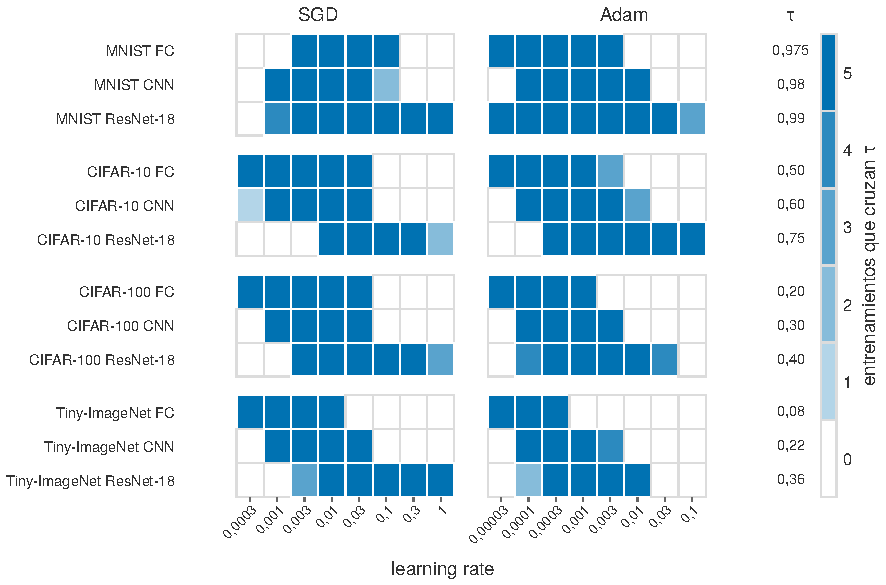
\includegraphics{ventana-lr}
\caption{Entrenamientos que cruzan el umbral en cada \emph{learning rate}, por celda.}
\label{fig:ventana-lr}
\end{figure}

La censura resulta así una consecuencia del diseño. Los extremos de la rejilla existen para producir entrenamientos malos, como expone la Sección~\ref{sec:matriz}, y son precisamente ellos los que no alcanzan el umbral. Descartar los entrenamientos censurados dejaría solo el centro de cada rejilla, y retiraría de la muestra la variación que la matriz se construyó para crear.

El nivel alcanzado cuadra con lo esperado. Tomando en cada celda el \emph{learning rate} cuya mediana de \emph{accuracy} de test sobre las cinco \emph{seeds} es mayor, nueve de las 12 combinaciones de conjunto y arquitectura caen dentro de la banda de la Tabla~\ref{tab:referencias}. La red \emph{fully connected} sobre CIFAR-10 llega al 57,8\,\%, por encima del 50 al 54\,\% esperado. La convolucional sobre CIFAR-100 se queda en el 39,0\,\%, por debajo del 45 al 55\,\%, y la ResNet-18 sobre CIFAR-10 en el 83,6\,\%, justo por debajo del 84 al 92\,\%.

\section{Rango dinámico del predictor}
\label{sec:res-rango}

Un coeficiente de correlación nulo admite tres lecturas que desde fuera no se distinguen. Puede que la métrica no prediga nada. Puede que el suceso a predecir ya hubiera ocurrido cuando se midió la métrica. O puede que la métrica no se mueva dentro de una celda más de lo que la mueve el ruido de la \emph{seed}. Esta sección descarta la tercera. Mide qué parte de la dispersión de cada columna registrada explica el \emph{learning rate} y qué parte explica la \emph{seed}. Es una comprobación del lado del predictor, sin consultar ninguna variable dependiente.

Dentro de una celda hay 40 entrenamientos, ocho \emph{learning rates} por cinco \emph{seeds}, y dentro de cada \emph{learning rate} lo único que cambia es la \emph{seed}. Los valores de una columna se sustituyen por su posición en la ordenación, del 1 al 40. La dispersión de esas posiciones se parte en dos, la que separa a los grupos entre sí y la que queda dentro de cada grupo:

\begin{equation}
\eta^2_{\mathrm{LR}} = \frac{\sum_{g} n_g\,(\bar{R}_g - \bar{R})^2}{\sum_{i} (R_i - \bar{R})^2},
\label{eq:eta-rangos}
\end{equation}

donde $R_i$ es la posición del entrenamiento $i$, $\bar{R}$ la media de todas las posiciones, $\bar{R}_g$ la media del grupo $g$ y $n_g$ su tamaño. El cociente vale 1 cuando el \emph{learning rate} explica toda la dispersión y 0 cuando las medias de los grupos coinciden. El mismo cociente se calcula agrupando por \emph{seed} en lugar de por \emph{learning rate}, y de ahí salen las dos cifras que se comparan. Trabajar sobre posiciones impide que un entrenamiento extremo domine el reparto, y hace la cifra comparable entre métricas cuyas unidades difieren en órdenes de magnitud.

El cociente no vale cero aunque el \emph{learning rate} no intervenga. Si se reparten $n$ posiciones al azar entre $k$ grupos, las medias de los grupos difieren algo por pura suerte, y el valor esperado del cociente es $(k-1)/(n-1)$. Esa es la referencia contra la que se lee cada cifra. Vale para cualquier conjunto fijo de valores, y trabajar con posiciones hace además que no dependa de cómo se distribuye la columna.

El estadístico no exige normalidad ni varianzas iguales, porque opera sobre posiciones y no contrasta ninguna hipótesis. Tampoco exige que la relación con el \emph{learning rate} sea monótona, porque trata los ocho valores como grupos sin orden. Lo que sí exige es la rejilla cruzada y completa de la Sección~\ref{sec:matriz}, que garantiza que dentro de un grupo solo cambie la \emph{seed}. Cada pareja de \emph{learning rate} y \emph{seed} tiene un solo entrenamiento, y no se puede saber si una \emph{seed} sale alta en todos los \emph{learning rates} o solo en algunos. Por eso las dos cifras se publican aparte y no como un reparto que sume uno.

La Figura~\ref{fig:rango-celda} recorre una celda completa, MNIST con la red convolucional y SGD, con la \emph{gradient disparity} medida al 5\,\% del presupuesto. Las medias de los ocho grupos se reparten por toda la escala. Dentro de un grupo, los cinco entrenamientos quedan en una banda más estrecha, que se ensancha donde la columna vale más. El panel derecho cambia cada valor por su posición dentro de la celda, de 1 el más bajo a 39 el más alto, que es la vista sobre la que opera la Ecuación~\ref{eq:eta-rangos}. Son 39 porque el entrenamiento divergido de la celda no deja valor en esta columna. Entre los 39 están los 12 que se quedaron en el azar, y la figura los marca aparte porque son parte de lo que hay que ver. El \emph{learning rate} explica 0,88 de la dispersión, frente a una referencia de 0,18 para sus ocho grupos. La \emph{seed} explica 0,08, por debajo de la referencia de 0,11 de sus cinco grupos, es decir, nada más allá del azar.

\begin{figure}[ht]
\centering
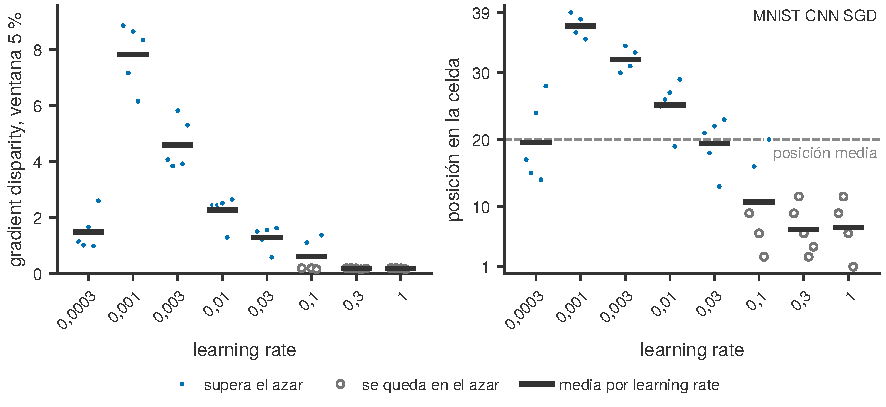
\includegraphics{rango-celda}
\caption{Una celda completa, MNIST con la red convolucional y SGD, al 5\,\%.}
\label{fig:rango-celda}
\end{figure}

El panel izquierdo muestra además una forma que el cociente no recoge. La columna sube hasta el \emph{learning rate} $10^{-3}$ y a partir de ahí baja, sin crecer ni decrecer de un extremo al otro de la rejilla. El cociente la puntúa alto igual, porque mide si hay estructura, no en qué sentido va. Un coeficiente de rangos, en cambio, solo detecta relaciones que suben o bajan en un único sentido, y leería la mitad de esa curva como ausencia de señal. Dentro de una celda, la relación entre una métrica y una variable es la composición de dos curvas sobre el \emph{learning rate}, y ningún estadístico de rangos la deshace. La Sección~\ref{sec:protocolo-analisis} declara las celdas donde esa relación no puede ser monótona y añade una lectura, la de selección, que no depende de la forma.

Cada métrica entra representada por su columna titular, la que fija la Tabla~\ref{tab:columnas-titulares}, porque las demás columnas de una métrica son otras lecturas de la misma cantidad (Sección~\ref{sec:variables}). La Figura~\ref{fig:rango-columnas} repite la cuenta en las 24 celdas al 5\,\% del presupuesto y resume cada columna por su mediana. Las ocho métricas de gradiente superan su referencia con holgura, desde 0,45 la más floja hasta 0,92 la que más. La cuenta se extiende a las cuatro ventanas tempranas. De las 768 casillas de métrica de gradiente, que son 24 celdas por cuatro ventanas por ocho columnas, solo 30 quedan en la referencia o por debajo, un 3,9\,\%. Todas corresponden a la familia de variabilidad o a la m-coherencia, que da exactamente el mismo número que la escala de ruido por la Ecuación~\ref{eq:gns-mcoh}. La tercera lectura de un coeficiente nulo queda descartada en casi toda la rejilla.

\begin{figure}[ht]
\centering
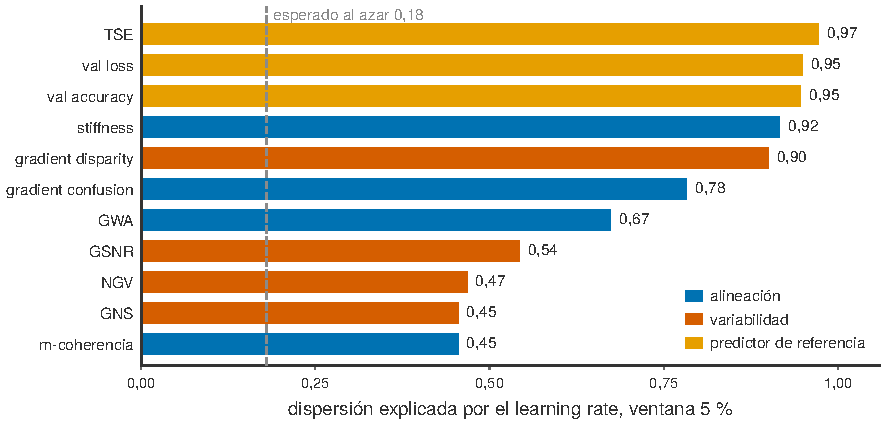
\includegraphics{rango-columnas}
\caption{Dispersión explicada por el \emph{learning rate} en las 24 celdas.}
\label{fig:rango-columnas}
\end{figure}

La parte que queda dentro de los \emph{learning rates} es el complemento de esa cifra, y es la única que puede usar la cuenta del contraste que fija el \emph{learning rate}, la granulada de la Sección~\ref{sec:protocolo-granulada}. Al 5\,\% es el 8\,\% de la dispersión en la \emph{stiffness}, el 10\,\% en la \emph{gradient disparity}, el 22\,\% en la \emph{gradient confusion} y el 33\,\% en GWA. En GSNR es el 46\,\% y en la escala de ruido el 55\,\%. En las tres lecturas del predictor de referencia (\emph{baseline}) queda entre el 3 y el 5\,\%. Las cuentas sobre las 24 celdas usan solo los entrenamientos que aprendieron, según el criterio de la Sección~\ref{sec:calibracion}, mientras que la celda de ejemplo muestra todos los que tienen valor. Repetir las 24 celdas al 5\,\% con todos los que tienen valor mueve las medianas menos de tres centésimas. Esa coincidencia no aísla el efecto de los entrenamientos que nunca aprendieron, porque quitarlos recorta también el extremo alto de la rejilla. Dice solo que el resultado no depende de qué población se elija.

Las tres columnas que encabezan la Figura~\ref{fig:rango-columnas} no cuestan nada de calcular. TSE marca 0,97 y las dos lecturas de la curva de validación 0,95, por encima del 0,92 de la métrica instrumentada que más se mueve. Dentro de una celda, la columna que mejor sigue al \emph{learning rate} es justamente la que no hay que pagar, y esa es la vara que la hipótesis H2 obliga a superar.

Ese mismo resultado deja medida la causa común que la Sección~\ref{sec:matriz} declara. Dentro de una celda, la métrica y el indicador de eficiencia responden los dos al \emph{learning rate}, y una correlación entre ellos mide en buena parte si la métrica es una relectura del \emph{learning rate} en el mismo sentido que el resultado. Por eso la posición en la rejilla entra en todas las tablas del contraste como predictor de coste cero, y la cuenta granulada de la Sección~\ref{sec:protocolo-granulada}, que solo compara entrenamientos con el mismo \emph{learning rate}, acompaña a cada recuento.

\section{Solape entre la ventana y el desenlace}
\label{sec:res-solape}

De las tres lecturas de un coeficiente nulo con las que abre la Sección~\ref{sec:res-rango} queda por acotar la segunda, que el suceso a predecir ya hubiera ocurrido al medir. La Sección~\ref{sec:ventana} lo enuncia como condición y la Sección~\ref{sec:riesgos} exige medir su alcance antes de interpretar cualquier resultado de velocidad. Esta sección lo mide celda a celda y ventana a ventana sobre las tres variables que se leen a lo largo de la curva de validación, las dos de velocidad y el mejor \emph{loss}, y dice qué ventanas conservan sentido para cada una. Como la anterior, trabaja sobre un solo lado, aquí el de las variables dependientes, y no consulta ninguna métrica.

Una ventana se cierra en la \emph{epoch} en la que se lee el predictor, la 1, 2, 5 y 10 en MNIST y la 2, 4, 10 y 20 en los otros tres conjuntos. Un suceso que ocurre en esa misma \emph{epoch} cuenta como ya pasado, porque la métrica y el suceso describen la misma red al final de la misma \emph{epoch}, y la primera no puede anticipar lo que ya es. El suceso de las \emph{epochs} hasta el umbral es el cruce. El del mejor \emph{loss} de validación es la \emph{epoch} en la que la curva suavizada toca su mínimo. El área bajo la curva no tiene suceso, porque es una suma ponderada de los \emph{loss} de todas las \emph{epochs}. Lo que la ventana deja atrás es la parte de esa suma que ya está fijada al cerrarse.

La unidad de la cuenta son los pares comparables, la misma con la que la Sección~\ref{sec:res-cobertura} mide la censura, porque un coeficiente de rangos consume pares. Un par sigue siendo una predicción cuando ninguno de sus dos entrenamientos ha tenido el suceso al cerrar la ventana, y un entrenamiento censurado nunca lo tiene. Con $k$ cruces en la celda, $f$ de ellos todavía por delante y $c$ entrenamientos censurados, la parte de los pares comparables que sigue por delante es
\begin{equation}
\frac{\binom{f}{2} + f\,c}{\binom{k}{2} + k\,c},
\label{eq:pares-delante}
\end{equation}
y para el mejor \emph{loss}, que nunca se censura, $c$ vale cero. Para el área, lo que queda por delante de cada entrenamiento es el complemento de la fracción ya fijada, y la celda se resume por su mediana.

Una ventana sirve para una variable en una celda cuando al menos la mitad de esa variable sigue por delante, porque entonces la ventana predice para la mayor parte de la información que usa el contraste. La regla se fijó después de conocer las cifras agregadas sobre los 960 entrenamientos y antes del desglose por celda, y se declara como lo que es, una regla posterior a los datos (Sección~\ref{sec:protocolo-cuando}). Desde la revisión del método la regla ya no decide qué celdas se leen, solo describe cuánto queda por delante en cada una. La velocidad se lee por hitos, entre los entrenamientos que aún no han cruzado al cerrar la ventana, según fija la Sección~\ref{sec:protocolo-hitos}.

La Figura~\ref{fig:solape-celda} recorre CIFAR-10 con la red convolucional y SGD, la celda que reparte sus cruces cinco a cinco entre las cuatro ventanas. Cada curva es el \emph{accuracy} de validación suavizado de un entrenamiento, la línea horizontal es el umbral y las cuatro verticales marcan la \emph{epoch} en la que cierra cada ventana. De sus 40 entrenamientos cruzan 21, y las cuatro ventanas dejan atrás cinco, 10, 15 y 20 de esos cruces. El panel inferior los cuenta acumulados, porque en las curvas se amontonan a la izquierda y el reparto no se ve. En pares, la parte que sigue por delante baja de 0,70 al 5\,\% a 0,43 al 10\,\%, 0,21 al 25\,\% y 0,03 al 50\,\%. A partir de la segunda ventana, lo que una métrica leída ahí puede hacer con la variable principal es, en su mayor parte, describir un cruce que ya ha pasado.

\begin{figure}[ht]
\centering
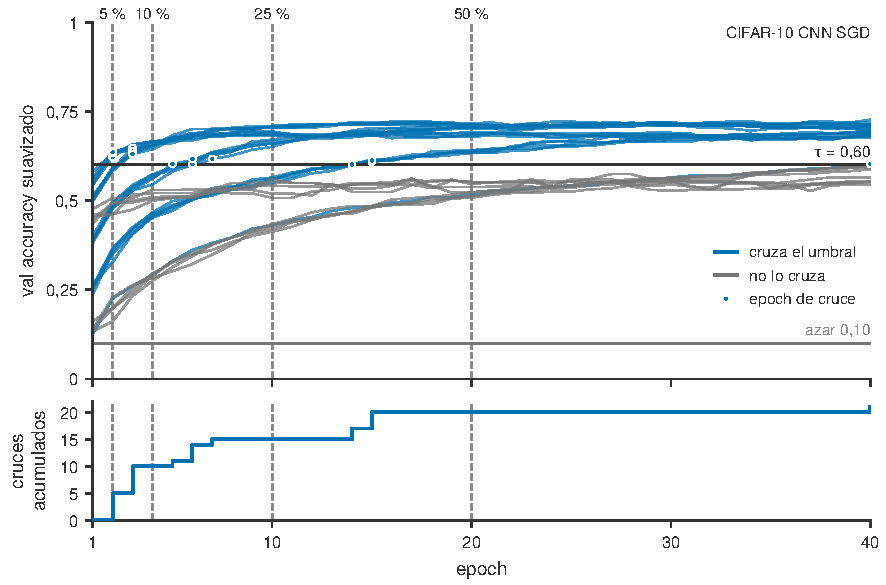
\includegraphics{solape-celda}
\caption{Cruces del umbral en CIFAR-10 con la red convolucional y SGD.}
\label{fig:solape-celda}
\end{figure}

Contado en entrenamientos y sumado sobre las 24 celdas, de los 573 cruces ya ha ocurrido el 10\,\% al cerrar la ventana del 5\,\% y el 35\,\% al cerrar la del 10\,\%. Al cerrar la del 25\,\% ha ocurrido el 72\,\%, y al cerrar la del 50\,\%, el 85\,\%. Esta cuenta va en entrenamientos, no en pares, y mide el tamaño del solape sin decidir nada.

El reparto entre conjuntos de datos confunde si se lee en fracción del presupuesto. La \emph{epoch} mediana de cruce es la 5 en MNIST, en CIFAR-10 y en Tiny-ImageNet, y la 4 en CIFAR-100. Los cuatro conjuntos cruzan a la misma altura absoluta. Lo que cambia es el presupuesto, 20 \emph{epochs} en MNIST frente a 40 en los demás, y la misma \emph{epoch} es en MNIST el doble de fracción. Las seis celdas de MNIST conservan la mitad por delante al 10\,\% porque su ventana del 10\,\% cierra en la \emph{epoch} 2, y la de los otros conjuntos en la 4. Seis de las 12 celdas que sirven al 10\,\% lo son por ese denominador. Por arquitectura, la red \emph{fully connected} cruza antes que las otras dos, con mediana en la \emph{epoch} 4 frente a 5 en la ResNet-18 y 6 en la convolucional. Tampoco ahí se separa la dificultad de la exigencia, porque a la red plana se le pide el umbral más bajo de las tres. Comparar el solape entre conjuntos mezcla tiempo absoluto y relativo. Dentro de una celda es constante.

Para las \emph{epochs} hasta el umbral, contadas celda a celda y en pares, la ventana del 5\,\% sirve en 22 celdas y la del 10\,\% en 12, y ninguna de las dos posteriores sirve en ninguna. Las dos celdas que fallan ya al 5\,\% son la red \emph{fully connected} con Adam en CIFAR-100 y en Tiny-ImageNet, donde más de la mitad de los cruces, 11 de 20 y 10 de 15, caen en las dos primeras \emph{epochs}. Al 10\,\% el reparto se parte por arquitectura. Quedan por encima de la mitad las seis celdas de MNIST, las cuatro de la convolucional y la ResNet-18 sobre Tiny-ImageNet y las dos de la ResNet-18 con SGD sobre CIFAR. Ninguna red \emph{fully connected} fuera de MNIST llega a la mitad, y la que más conserva, Tiny-ImageNet con SGD, se queda en 0,42. Es el mismo orden por profundidad que dibuja la Figura~\ref{fig:ventana-lr}, porque a la red plana se le pide el umbral más bajo y lo alcanza antes.

El mejor \emph{loss} de validación conserva más ventanas, 24 celdas al 5\,\%, 17 al 10\,\%, nueve al 25\,\% y dos al 50\,\%, y lo que lo consume es el sobreajuste. Sin \emph{data augmentation} ni \emph{weight decay}, la curva de \emph{loss} de validación toca fondo pronto y vuelve a subir (Sección~\ref{sec:setup}). En CIFAR-10 con ResNet-18 y Adam, 37 de los 40 entrenamientos tocan fondo en la \emph{epoch} 10 o antes y el último en la 14, y al 25\,\% queda por delante el 0,4\,\% de los pares. En esas celdas el suceso de esta variable es el inicio del sobreajuste, y así hay que leerla.

El comportamiento del área bajo la curva es casi mecánico. Al cerrar cada ventana queda fijada casi exactamente la fracción del presupuesto transcurrida, con medianas de 0,96, 0,90, 0,76 y 0,51 por delante, frente a los 0,96, 0,91, 0,76 y 0,50 que dejaría una curva plana de 40 \emph{epochs}. Lo dictan los pesos de la suma, sin que los datos aporten nada. La variable sirve hasta el 25\,\% en las 24 celdas. Al 50\,\% cae sobre la línea por construcción, con 13 celdas de 24, y para esa ventana queda declarada como descrita a medias.

Las cuentas anteriores usan los 960 entrenamientos. Repetidas solo con los que aprendieron, según el criterio de la Sección~\ref{sec:calibracion}, el recuento de celdas del área no cambia. El de las \emph{epochs} hasta el umbral pierde una celda al 5\,\%, y el del mejor \emph{loss} se mueve una celda al 5, al 10 y al 50\,\%. Un entrenamiento que nunca aprende nunca cruza, entra como censurado, y quitarlo apenas toca el reparto.

Para las variables de velocidad, el barrido de ventanas de la hipótesis H4 queda acotado a las del 5 y el 10\,\%. Se declara en \emph{epochs}, la 1 frente a la 2 en MNIST y la 2 frente a la 4 en los demás conjuntos. Las tres variables que se miden al terminar el entrenamiento no tienen este límite. La cuenta es además un suelo. Un entrenamiento al 95\,\% del umbral al cerrar la ventana tiene el desenlace casi escrito y aquí cuenta como por delante. El solape real es mayor que el medido. La Sección~\ref{sec:protocolo-hitos} fija qué hace el contraste con los entrenamientos que ya han cruzado, que es dejarlos fuera de la lectura primaria de la velocidad. La cuenta de esta sección solo describe cuánto queda por delante en cada celda. El solape favorece además al predictor de referencia. En un entrenamiento que ya cruzó, el \emph{accuracy} de validación leído en la ventana vale ya el umbral, y lo detecta sin coste. Por eso H2 no se decide sobre la velocidad, según fija la Sección~\ref{sec:protocolo-eval}.

\section{Concordancia entre validación y test}
\label{sec:res-val-test}

Las variables de velocidad se leen sobre la curva de validación, y el test se evalúa una sola vez al terminar, como fija la Sección~\ref{sec:protocolo-eval}. Lo que este trabajo afirme sobre velocidad descansa por tanto en que la validación cuente lo mismo que el test. El diseño lo hace esperable, porque las dos particiones salen del mismo origen y ninguna interviene en el entrenamiento. Esta sección lo comprueba en el único instante en que las dos lecturas coexisten, el final del entrenamiento, sobre los 919 entrenamientos que no divergieron. Es una correlación entre dos variables dependientes y tampoco consulta ninguna métrica.

Se comparan dos cosas, el orden y el nivel. El orden importa porque los contrastes de la Sección~\ref{sec:protocolo-analisis} ordenan los entrenamientos de una celda. El nivel importa porque el umbral de la Sección~\ref{sec:calibracion} se fijó sobre validación. El orden se mide con la tau de Kendall dentro de cada celda, que cuenta los pares de entrenamientos que las dos lecturas ordenan igual, resta los que ordenan al revés y divide por el total de pares. Su mediana sobre las seis celdas de cada conjunto es 0,93 en los dos CIFAR, 0,92 en Tiny-ImageNet y 0,84 en MNIST para el \emph{accuracy}, y entre 0,86 y 0,94 para el \emph{loss}. Las 24 celdas caen entre 0,71 y 0,97. El mínimo es MNIST con ResNet-18 y Adam, cuyos 40 entrenamientos terminan en un tramo de 0,008 de \emph{accuracy} de test, del tamaño del ruido de medida, y con esa separación el orden es ruido en las dos lecturas a la vez. Lo mismo ocurre en cinco de las seis celdas de MNIST entre los entrenamientos que aprendieron y no divergieron, que terminan a menos de cinco centésimas unos de otros. Es un aviso para los contrastes sobre el rendimiento final, porque en MNIST esa variable apenas tiene recorrido entre los entrenamientos sanos. El nivel es la diferencia validación menos test de cada entrenamiento, leída contra el ruido de medir el \emph{accuracy} sobre un número finito de ejemplos. Su mediana es 0,003 en CIFAR-10 y cero en los otros tres conjuntos, y el 95\,\% de los entrenamientos queda a menos de 0,011 de la igualdad. Los que se separan más de dos desviaciones típicas del ruido van del 0\,\% en Tiny-ImageNet al 1,8\,\% en CIFAR-10, por debajo del 4,6\,\% que el ruido solo produciría, porque los entrenamientos clavados en el azar dan el mismo \emph{accuracy} en las dos particiones.

La misma evaluación cierra la comprobación anunciada en la Sección~\ref{sec:protocolo-eval}. La diferencia entre la F1 macro y el \emph{accuracy} de test tiene mediana 0,002. Entre los 804 entrenamientos que aprendieron y no divergieron, el 95\,\% queda por debajo de 0,018 y el máximo es 0,071. Repetidas solo con los entrenamientos que aprendieron, las medianas de la tau bajan menos de tres centésimas, porque desaparecen los empates del azar, y el nivel no cambia. La curva de validación es una lectura fiel del test en orden y en nivel, y las variables de velocidad que se leen sobre ella no son un artefacto de la partición. Lo que no se puede establecer es el acuerdo en cada \emph{epoch}, porque el test se mira una sola vez.

\section{Existencia de la asociación}
\label{sec:res-por-condicion}
% Escrita el 2026-09-03 (fase B, paso 4) y reescrita esa misma tarde con el método revisado.
% Números de results/tabla_larga.parquet, regenerable con `uv run python src/contrast.py`;
% figura signos-h1 en src/figures.py. H1 se lee como requisito previo, no como hallazgo. La lectura de
% selección (results/seleccion.parquet) es de H2 y va en §Valor incremental.

Esta sección responde a la hipótesis H1, la de existencia, sobre la familia primaria que fija la Sección~\ref{sec:protocolo-agregacion}. La familia es la ventana del 5\,\%, tres variables y diez predictores. Las variables son las \emph{epochs} hasta el umbral leídas por hitos (\emph{landmark}), es decir, solo entre los entrenamientos que aún no habían cruzado al cerrar la ventana, el \emph{accuracy} de test y el \emph{gap} de \emph{loss}. Los predictores son la posición en la rejilla, las tres lecturas del predictor de referencia y las seis métricas de gradiente que quedan tras la poda. Cada D se calcula dentro de una celda, sobre los entrenamientos que aprendieron. D vale 1 cuando el predictor ordena los entrenamientos igual que la variable, $-1$ cuando los ordena al revés y 0 cuando acierta tantos pares como falla. Cada D lleva su intervalo por \emph{jackknife}, y una celda muestra asociación cuando ese intervalo deja fuera el cero. La Tabla~\ref{tab:signos-h1} da, para cada combinación, cuántas celdas tienen D positiva y cuántas negativa, cuántas de cada signo muestran asociación, y el mismo recuento de signos para la cuenta granulada, la que compara solo entrenamientos con el mismo \emph{learning rate}. En el texto, el número de celdas de un predictor es el de las que muestran asociación con su signo mayoritario, el signo que su D tiene en más celdas; la tabla da también las del signo contrario. La Figura~\ref{fig:signos-h1} resume las 24 D de cada combinación en una caja. La raya es la mediana, la caja abarca la mitad central de las celdas y los bigotes van de la celda más baja a la más alta. Las cajas de las tres lecturas del predictor de referencia quedan lejos del cero con la velocidad y con el \emph{accuracy} de test, y con el \emph{gap} cruzan el cero y son anchas. Las cajas de las seis métricas cruzan el cero, con tres excepciones, GWA con la velocidad y con el \emph{accuracy} de test y la \emph{stiffness} con el \emph{gap}.

\begin{figure}[ht]
\centering
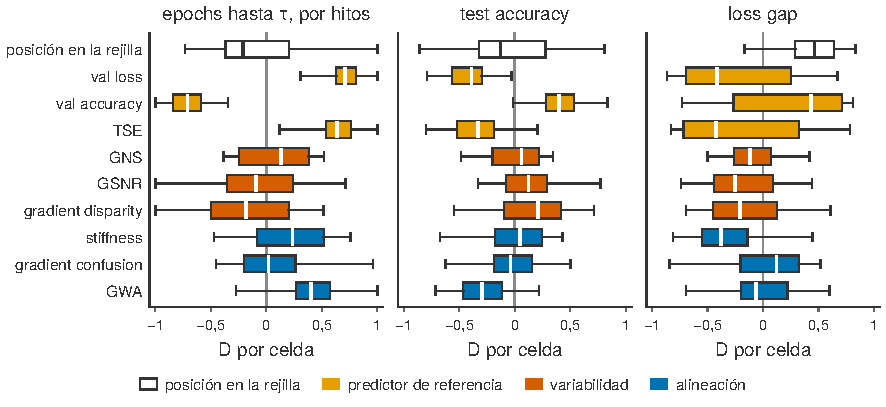
\includegraphics{signos}
\caption{D por celda de la familia primaria al 5\,\%.}
\label{fig:signos-h1}
\end{figure}

\begin{table}[ht]
\centering
\footnotesize
\setlength{\tabcolsep}{3.5pt}
\caption{Recuento de celdas de la familia primaria. En negrita, las combinaciones con asociación del mismo signo en 15 celdas o más.}
\label{tab:signos-h1}
\begin{tabular}{lccccccccc}
\toprule
& \multicolumn{3}{c}{\textbf{\emph{Epochs} hasta el umbral}} & \multicolumn{3}{c}{\textbf{\emph{Accuracy} de test}} & \multicolumn{3}{c}{\textbf{\emph{Gap} de \emph{loss}}} \\
\cmidrule(lr){2-4}\cmidrule(lr){5-7}\cmidrule(lr){8-10}
\textbf{Predictor} & $+/-$ & asoc. & gran. & $+/-$ & asoc. & gran. & $+/-$ & asoc. & gran. \\
\midrule
Posición en la rejilla & 9/15 & 5/7 & 0/0 & 11/13 & 6/7 & 0/0 & 21/3 & \textbf{15/0} & 0/0 \\
\emph{Loss} de validación & 24/0 & \textbf{24/0} & 16/6 & 0/24 & \textbf{0/19} & 4/18 & 7/17 & \textbf{6/16} & 7/16 \\
\emph{Accuracy} de validación & 0/24 & \textbf{0/24} & 5/18 & 23/1 & \textbf{18/0} & 19/5 & 17/7 & \textbf{16/6} & 15/8 \\
TSE & 24/0 & \textbf{23/0} & 16/6 & 1/23 & \textbf{0/17} & 7/17 & 8/16 & \textbf{7/16} & 11/12 \\
\addlinespace
GNS & 14/10 & 7/3 & 11/12 & 14/10 & 3/6 & 9/12 & 9/15 & 5/6 & 15/9 \\
GSNR & 11/13 & 6/7 & 11/11 & 15/9 & 7/4 & 13/9 & 8/16 & 2/11 & 6/16 \\
\emph{Gradient disparity} & 9/15 & 4/9 & 9/12 & 15/9 & 12/4 & 13/10 & 9/15 & 4/11 & 14/7 \\
\addlinespace
\emph{Stiffness} & 15/8 & 9/5 & 14/8 & 12/12 & 5/6 & 13/11 & 4/20 & \textbf{1/15} & 10/12 \\
\emph{Gradient confusion} & 12/12 & 5/4 & 10/10 & 11/13 & 5/5 & 18/6 & 14/10 & 9/5 & 7/13 \\
GWA & 21/3 & \textbf{16/1} & 9/13 & 4/20 & \textbf{1/15} & 7/16 & 8/16 & 6/4 & 11/11 \\
\bottomrule
\end{tabular}
\end{table}

Antes de leer los signos, el protocolo pide declarar tres cifras de la población. En los contrastes del \emph{gap} entran solo los entrenamientos que alcanzaron el umbral de su celda sobre el conjunto de entrenamiento, y son 693 de los 806, con 25 por celda de mediana. Cinco celdas conservan los 40 y tres se quedan en 20, Tiny-ImageNet con la red \emph{fully connected} y con la convolucional bajo Adam, y MNIST con la red \emph{fully connected} bajo SGD. Al cerrar la ventana del 5\,\% quedan por cruzar entre 15 y 40 entrenamientos por celda, la mitad de las celdas con 30 o más, y entre 50 y 713 pares comparables, 366 de mediana. Las dos celdas con menos entrenamientos en riesgo son la red \emph{fully connected} bajo Adam sobre Tiny-ImageNet, con 15, y sobre CIFAR-100, con 17, las mismas que la Sección~\ref{sec:res-solape} señala. Queda la forma de las curvas. El protocolo advierte de que D no puede ver una relación cuando el predictor solo sube o solo baja a lo largo del \emph{learning rate} y la variable pasa por un pico o un valle. Esas celdas son pocas para todos los predictores. La \emph{stiffness} es la peor, con seis en velocidad, siete en \emph{accuracy} de test y cinco en el \emph{gap}. La escala de ruido, GSNR y la \emph{gradient confusion} tienen entre dos y cuatro, y la disparidad y GWA entre dos y tres.

La posición en la rejilla es el logaritmo del \emph{learning rate}, y marca el techo de lo que una lectura monótona del \emph{learning rate} puede dar. Con la velocidad muestra asociación en 12 celdas en total y con el \emph{accuracy} de test en 13, pero repartidas casi por igual entre los dos signos, cinco positivas y siete negativas en la primera, seis y siete en la segunda. Con su signo mayoritario son siete y siete. Las dos variables pasan por un valle o por un pico a lo largo de la rejilla, y el signo depende de a qué lado del óptimo caigan los \emph{learning rates} de la celda. Con el \emph{gap} de \emph{loss} la relación sí es monótona. Un \emph{learning rate} mayor acompaña a un \emph{gap} mayor, y la posición muestra asociación positiva en 15 celdas y negativa en ninguna, cinco por arquitectura.

Las tres lecturas del predictor de referencia ordenan los entrenamientos de casi todas las celdas. El \emph{accuracy} de validación muestra asociación negativa con las \emph{epochs} hasta el umbral en las 24 celdas, y el \emph{loss} de validación y TSE positiva en 24 y en 23, con medianas de 0,64 a 0,71 en valor absoluto. Con el \emph{accuracy} de test el signo se invierte, como corresponde, en 18, 19 y 17 celdas, con medianas de 0,33 a 0,40 y sin ninguna celda del signo contrario. Con el \emph{gap} de \emph{loss} los tres se parten, y el corte es la arquitectura. En las ocho celdas de la red \emph{fully connected} y en las ocho de la convolucional, un \emph{loss} de validación alto en la ventana acompaña a un \emph{gap} menor al terminar, con asociación en las 16. En la ResNet-18 acompaña a un \emph{gap} mayor, con asociación en seis de las ocho. El \emph{accuracy} de validación dibuja lo mismo con el signo opuesto. Contadas las 24 celdas juntas, las dos relaciones se anulan.

De las seis métricas de gradiente, dos superan a la posición en la rejilla en alguna variable y una la iguala. GWA muestra asociación positiva con las \emph{epochs} hasta el umbral en 16 celdas y negativa en una, con mediana 0,40, y negativa con el \emph{accuracy} de test en 15 y positiva en una, con mediana $-0{,}29$. Una GWA alta en la ventana acompaña a un entrenamiento más lento y a un \emph{accuracy} final menor, en los cuatro conjuntos de datos y en las tres arquitecturas. La única celda de signo contrario es, en las dos variables, la ResNet-18 sobre Tiny-ImageNet con SGD. La \emph{gradient disparity} muestra asociación positiva con el \emph{accuracy} de test en 12 celdas y negativa en cuatro, con mediana 0,21. Las seis celdas de la convolucional y cinco de la red plana van en el mismo sentido. Las cuatro contrarias son dos de la red plana, sobre CIFAR-10 y sobre MNIST, y dos de la ResNet-18, sobre MNIST y sobre Tiny-ImageNet. La \emph{stiffness} muestra asociación negativa con el \emph{gap} de \emph{loss} en 15 celdas y positiva en una, con mediana $-0{,}38$. Una \emph{stiffness} alta acompaña a un \emph{gap} menor en las 13 celdas con asociación de la red plana y de la convolucional, y la ResNet-18 se parte. Son 15 celdas frente a las 15 de la posición en la rejilla, y la \emph{stiffness} iguala al \emph{learning rate} leído de otra forma, sin superarlo. Las otras tres métricas no superan a la posición en ninguna variable. GSNR empata con ella a siete celdas en velocidad y en \emph{accuracy} de test, y la escala de ruido a siete en velocidad; en los tres empates la posición queda delante por la mediana de $|D|$. En el resto de casos las tres quedan por debajo, con entre tres y 11 celdas. Su signo cambia además con el conjunto de datos o con la arquitectura. GSNR va con la velocidad en un sentido en CIFAR-10 y en el contrario en MNIST, y la escala de ruido se asocia con la velocidad sobre todo en la ResNet-18 y casi nada en la red plana.

La cuenta granulada deja la tabla casi vacía. Compara solo entrenamientos con el mismo \emph{learning rate}, es decir, las cinco \emph{seeds} de cada uno, y el \emph{learning rate} no puede mover la D. Ninguna de las 30 combinaciones muestra asociación en más de tres celdas, y las celdas que la muestran no coinciden de una variable a otra ni de una métrica a otra. Los recuentos de signo bajan a lo que una moneda da con frecuencia. Para las métricas de gradiente, el signo más frecuente reúne entre 10 y 16 celdas, con una excepción sin intervalo, la \emph{gradient confusion} con el \emph{accuracy} de test, 18 de 24. Las lecturas del predictor de referencia llegan a 18 y 19 con esa misma variable y con la velocidad, también sin intervalo fuera del cero en más de tres celdas. Las medianas del valor absoluto bajan a entre 0,10 y 0,33 en las seis métricas, y a 0,43 como mucho en el predictor de referencia, frente a los 0,18 a 0,71 de la cuenta por celda. La posición en la rejilla da cero en todas, porque dentro de un \emph{learning rate} no tiene nada que ordenar. Dentro de un \emph{learning rate}, ninguna métrica ordena las cinco \emph{seeds} mucho mejor que el azar, y eso vale también para el predictor de referencia. Lo que la cuenta por celda recoge es, en su mayor parte, que el \emph{learning rate} mueve a la vez la métrica y la eficiencia, según anticipó la Sección~\ref{sec:res-rango}.

H1 se sostiene como requisito previo, y solo por GWA. GWA muestra asociación con la velocidad en 16 celdas y con el \emph{accuracy} de test en 15, frente a las siete y siete de la posición en la rejilla, y con el mismo signo en los cuatro conjuntos de datos. Contando también las celdas del signo contrario, la ventaja se mantiene, 17 frente a 12 y 16 frente a 13. Las dos cuentas se dan porque la posición en la rejilla no cambia con la \emph{seed}. Su intervalo no es comparable con el de una métrica, y el requisito no puede depender de cómo se lea ese intervalo. La \emph{gradient disparity} supera también a la posición con el \emph{accuracy} de test, 12 frente a siete, pero su signo se da la vuelta en MNIST, con dos celdas negativas frente a una positiva, allí donde la variable apenas tiene recorrido. Con eso, las cinco hipótesis restantes tienen objeto. La asociación que sostiene H1 es, con todo, la que el \emph{learning rate} produce en las dos variables a la vez, y desaparece al fijarlo. Si esa asociación añade algo a lo que el \emph{loss} y el \emph{accuracy} de validación ya dicen en la misma ventana, sin coste, es la pregunta de H2. La D entre cada métrica y su referencia dentro de la celda ya avisa de que GWA y la \emph{stiffness} ordenan los entrenamientos en parte como el \emph{accuracy} de validación, con medianas de $-0{,}45$ y $-0{,}44$.

\section{Valor incremental sobre la referencia}
\label{sec:res-incremental}
% Fase C, escrita el 2026-09-04. Números de results/incremental.parquet y results/seleccion.parquet
% (2026-09-04), regenerables con `uv run python src/contrast.py`; figura `seleccion` en src/figures.py.

Esta sección responde a la hipótesis H2, la decisiva, con las tres lecturas de la Sección~\ref{sec:protocolo-objetivos}. La familia es la misma, la ventana del 5\,\% y los entrenamientos que aprendieron. Cada métrica se compara con la referencia nombrada de antemano para su variable, el \emph{accuracy} de validación para el \emph{accuracy} de test y el \emph{loss} de validación para el \emph{gap} de \emph{loss}. La primera lectura compara, celda a celda, el valor absoluto de la D de la métrica con el de su referencia. Cuenta en cuántas celdas la métrica gana y en cuántas pierde, y en cuántas de cada lado la diferencia deja fuera el cero por su intervalo \emph{jackknife}, calculado sobre los mismos entrenamientos. La segunda lee la D entre la métrica y su referencia dentro de la celda, $D_{\mathrm{ref}}$. Una métrica es redundante, es decir, la referencia con otro nombre, cuando el valor absoluto de esa D llega a 0,8, el umbral de la poda. La tercera es la lectura de selección de la Sección~\ref{sec:protocolo-seleccion}, la pérdida que la literatura de búsqueda de hiperparámetros llama \emph{regret}. En cada celda y \emph{seed} se elige el \emph{learning rate} que el predictor al 5\,\% señala como mejor, y se mide cuánto \emph{accuracy} de test se pierde frente al mejor \emph{learning rate} de esa \emph{seed}. La tabla da al lado, para cada predictor, en cuántas celdas esa pérdida es menor que la del \emph{accuracy} de validación, la columna «$<$ valid.». La posición en la rejilla no entra en esta lectura, porque elegir siempre el \emph{learning rate} más alto o el más bajo no es una predicción. La Tabla~\ref{tab:h2} recoge las tres lecturas para las dos variables que deciden, y la Figura~\ref{fig:seleccion} la tercera.

\begin{table}[ht]
\centering
\footnotesize
\setlength{\tabcolsep}{3.5pt}
\caption{H2 en la familia primaria. En negrita, la mejor métrica de gradiente en los recuentos crudos y en la selección.}
\label{tab:h2}
\begin{tabular}{lcccccccc}
\toprule
& \multicolumn{3}{c}{\textbf{\emph{Accuracy} de test}} & \multicolumn{3}{c}{\textbf{\emph{Gap} de \emph{loss}}} & \multicolumn{2}{c}{\textbf{Selección}} \\
\cmidrule(lr){2-4}\cmidrule(lr){5-7}\cmidrule(lr){8-9}
\textbf{Predictor} & gana/pierde & interv. & $|D_{\mathrm{ref}}|$ & gana/pierde & interv. & $|D_{\mathrm{ref}}|$ & pérdida & $<$ valid. \\
\midrule
Posición en la rejilla & 11/13 & 3/6 & 0,40 & 7/16 & 1/5 & 0,46 & & \\
\emph{Loss} de validación & 15/7 & 0/0 & 0,93 & ref. & ref. & ref. & 0,015 & 5 \\
\emph{Accuracy} de validación & ref. & ref. & ref. & 14/9 & 2/0 & 0,92 & 0,013 & ref. \\
TSE & 4/19 & 0/3 & 0,83 & 14/9 & 3/1 & 0,81 & 0,015 & 6 \\
\addlinespace
GNS & 6/18 & 0/8 & 0,26 & 3/21 & 0/12 & 0,25 & 0,073 & 0 \\
GSNR & 6/18 & 1/9 & 0,32 & 5/19 & 0/10 & 0,34 & 0,035 & 3 \\
\emph{Gradient disparity} & 10/14 & 3/8 & 0,36 & 5/18 & 0/7 & 0,37 & 0,097 & 1 \\
\addlinespace
\emph{Stiffness} & 5/19 & 0/8 & 0,44 & \textbf{7/17} & 2/6 & 0,44 & 0,110 & 1 \\
\emph{Gradient confusion} & 6/17 & 2/12 & 0,23 & 6/18 & 0/7 & 0,46 & 0,059 & 2 \\
GWA & \textbf{11/13} & 0/8 & 0,45 & 5/19 & 0/14 & 0,41 & \textbf{0,023} & \textbf{9} \\
\bottomrule
\end{tabular}
\end{table}

Sobre el \emph{accuracy} de test ninguna métrica gana a la validación. Con el recuento crudo la mejor es GWA, que gana en 11 celdas y pierde en 13, seguida de la \emph{gradient disparity} con 10 y 14; las otras cuatro ganan en cinco o seis. Con el intervalo el empate desaparece. GWA no gana con intervalo en ninguna celda y pierde en ocho. La disparidad es la única con tres celdas ganadas con intervalo, y pierde en ocho. Ninguna métrica es la validación con otro nombre. La mediana de $|D_{\mathrm{ref}}|$ va de 0,23 a 0,45, y solo dos celdas, las dos de GSNR, llegan a 0,8. Las métricas ordenan los entrenamientos de otra manera que la validación, y peor. Sin las seis celdas de MNIST, donde la variable apenas tiene recorrido, GWA queda en nueve celdas ganadas y nueve perdidas, ninguna con intervalo a favor y cinco en contra. La posición en la rejilla, que no hay que medir, hace lo mismo que la mejor métrica, 11 frente a 13. Dentro del predictor de referencia, las dos lecturas de la validación son intercambiables, con $|D_{\mathrm{ref}}|$ de 0,93 y las 24 celdas en 0,8 o más. TSE es redundante con el \emph{accuracy} de validación en 17 celdas y pierde contra él en 19. Los tres son una sola lectura.

Sobre el \emph{gap} de \emph{loss} la distancia es mayor. La referencia, el \emph{loss} de validación en la ventana, tiene una $|D|$ mediana de 0,54, y las seis métricas quedan entre 0,21 y 0,39. La \emph{stiffness} gana en siete celdas y pierde en 17, con dos ganadas y seis perdidas con intervalo. GWA gana en cinco y pierde en 19, con 14 perdidas con intervalo. El único predictor que supera a la referencia en el \emph{gap} es TSE, el \emph{loss} de entrenamiento acumulado, con 14 celdas frente a nueve y tres con intervalo frente a una. Los dos son gratuitos y los dos son lecturas de la velocidad, que a presupuesto fijo es en buena parte lo que el \emph{gap} mide, según la Sección~\ref{sec:variables}.

\begin{figure}[ht]
\centering
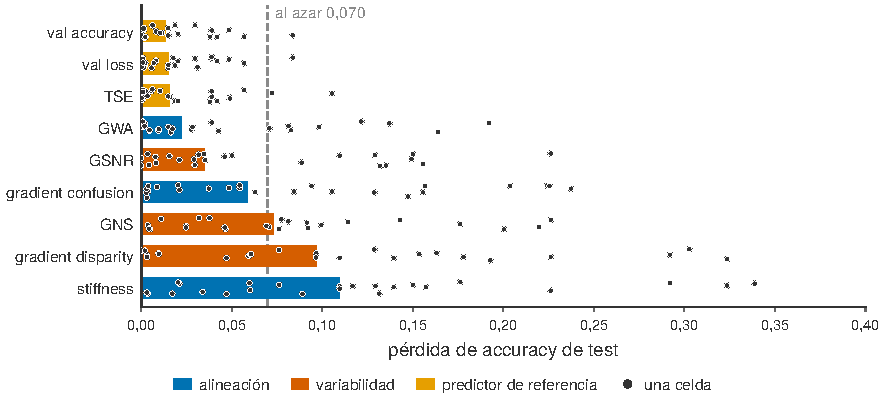
\includegraphics{seleccion}
\caption{Pérdida de \emph{accuracy} de test por selección al 5\,\%.}
\label{fig:seleccion}
\end{figure}

La lectura de selección, en la Figura~\ref{fig:seleccion}, pone la misma respuesta en puntos de \emph{accuracy}. Cada barra es la mediana sobre las 24 celdas y cada punto una celda. Elegir el \emph{learning rate} con el \emph{accuracy} de validación al 5\,\% pierde 0,013 frente al mejor de la celda; con el \emph{loss} de validación se pierde 0,015 y con TSE 0,015. Elegir al azar pierde 0,070. La mejor métrica es GWA, con 0,023, que pierde menos que la validación en nueve celdas repartidas entre los cuatro conjuntos. GSNR pierde 0,035 y la \emph{gradient confusion} 0,059. Las otras tres, con el signo que su artículo llama bueno, pierden más que elegir al azar, la escala de ruido 0,073, la disparidad 0,097 y la \emph{stiffness} 0,110. La cuenta con el signo invertido es una lectura a posteriori, sin regla previa, y se da como exploratoria. Con ella la disparidad baja a 0,023, la escala de ruido a 0,066 y la \emph{stiffness} a 0,075, y GWA, GSNR y la confusión suben a 0,084 o más. Para tres métricas el signo del artículo es el correcto en estas condiciones y para las otras tres es el contrario. Es lo mismo que H1 dejó ver en la disparidad, cuya D con el \emph{accuracy} de test es positiva.

Sobre la velocidad, donde H2 no decide, la referencia gana en todas partes. Ninguna métrica supera al \emph{accuracy} de validación al 5\,\% en más de cuatro celdas, y con intervalo pierden entre 13 y 19. El \emph{loss} de validación empata con él, 10 frente a 11, y TSE pierde en 21. Es lo que anuncia la Sección~\ref{sec:protocolo-eval}. La referencia es el primer tramo de la misma curva cuyo cruce se predice, y lleva ventaja por construcción.

H2 cae. En la ventana del 5\,\% ninguna métrica de gradiente supera a la lectura gratuita de la validación sobre el \emph{accuracy} de test ni sobre el \emph{gap}, ni con el intervalo de la diferencia ni eligiendo el \emph{learning rate} con ella. La que más se acerca, GWA, empata en el recuento crudo, pierde con intervalo y cuesta 0,023 de \emph{accuracy} frente a 0,013. Las métricas no son la validación con otro nombre, y aun así no la superan, porque lo que ordenan es el \emph{learning rate}, igual que la posición en la rejilla, que empata con la mejor de ellas. Si añaden algo encima de la validación, una vez fijada esta, no lo mide este diseño. La única cuenta libre del \emph{learning rate}, la granulada, queda vacía para todas, y también para la validación. El veredicto vale para esta ventana y esta rejilla. Qué pasa con ventanas posteriores lo mide la Sección~\ref{sec:res-temporal}, y lo que cuesta la instrumentación, la Sección~\ref{sec:res-coste}.

\section{Coste y capacidad predictiva}
\label{sec:res-coste}
% Fase C, escrita el 2026-09-04. Clases de coste de tab:coste-metricas; sobrecoste medido de
% desarrollo.tex §Cálculo de las métricas; capacidad predictiva de tab:h2.

La Tabla~\ref{tab:coste-metricas} separa los predictores en tres clases de coste. La clase gratuita reúne el \emph{loss} y el \emph{accuracy} de validación, TSE y la posición en la rejilla, que el entrenamiento produce sin calcular ningún gradiente. La clase del barrido compartido reúne cinco de las seis métricas de gradiente que quedan tras la poda. Las cinco calculan el gradiente de cada ejemplo del \emph{batch} de medición una sola vez, en un barrido común, y se separan después por la aritmética que hacen con él. Esa aritmética crece con el número de parámetros en la escala de ruido y GSNR, con el tamaño del \emph{batch} en GWA, y con el cuadrado del tamaño del \emph{batch} en la \emph{stiffness} y la \emph{gradient confusion}. La tercera clase es la de las submuestras, y solo tiene a la \emph{gradient disparity}, que sigue pagando sus cinco pasadas propias. Medido en reloj y sumado sobre los 960 entrenamientos, la instrumentación costó una cuarta parte del tiempo de entrenamiento. Por celda va del 0,7\,\% en la red convolucional sobre Tiny-ImageNet al 105\,\% en la red \emph{fully connected} sobre CIFAR-100 con SGD, es decir, hasta el doble del tiempo de entrenar, según mide la Sección~\ref{sec:des-metricas}. Ese reloj no separa una métrica de otra, porque el barrido es común.

Contra ese coste, la Tabla~\ref{tab:h2} no muestra ninguna métrica que supere a la clase gratuita. Dentro de la clase del barrido, la mejor sobre el \emph{accuracy} de test es GWA, la de aritmética más ligera. Empata con la posición en la rejilla y pierde con intervalo contra la validación. Sobre el \emph{gap} la mejor es la \emph{stiffness}, de coste cuadrático, con siete celdas ganadas frente a 17 perdidas. La disparidad, la única que paga pasadas propias, casi iguala a GWA en el recuento crudo del \emph{accuracy} de test y pierde en todo lo demás. Pagar más aritmética no compra orden. Eso responde a OE2. En la ventana del 5\,\% ninguna clase de coste compra más capacidad predictiva que la clase gratuita, y el sobrecoste, hasta el doble del tiempo de entrenamiento en la red plana, no está justificado como predicción. Lo que sí justifica es medir, que es lo que este trabajo hace con él, porque la serie completa por \emph{epoch} es la que permite responder a las hipótesis restantes.

\section{Qué familia predice mejor}
\label{sec:res-familia}
% Fase D, escrita el 2026-09-04. Números de results/ranking.parquet y ranking_grupos.parquet
% (2026-09-04), regenerables con `uv run python src/contrast.py`; las tres parejas de la poda las
% imprime `uv run python src/efficiency.py`. Sin figura: una comparación de niveles va a tabla.

Esta sección responde a la hipótesis H3 con la regla de la Sección~\ref{sec:protocolo-objetivos}. Para cada variable de la familia primaria, las seis métricas de gradiente se ordenan en un \emph{ranking} por el número de celdas en las que muestran asociación con su signo mayoritario, y a igualdad por la mediana del valor absoluto de D. No se calcula nada nuevo, porque las tres cifras salen de la Tabla~\ref{tab:signos-h1}, y la familia de cada métrica solo etiqueta el orden. La Tabla~\ref{tab:h3} da los tres órdenes, con la posición en la rejilla intercalada en el puesto que le tocaría y sin número. Contar solo las celdas del signo mayoritario penaliza a la métrica que cambia de sentido de una celda a otra, y debe hacerlo. Un predictor que ordena en un sentido en unas celdas y en el contrario en otras no sirve sin saber antes en qué celda se está. La escala de ruido, por ejemplo, muestra asociación negativa con el \emph{accuracy} de test en seis celdas y positiva en tres, pero su D es positiva en 14 celdas de 24, así que su signo mayoritario es el positivo y puntúa tres. La regla de tomar el signo mayoritario sobre las 24 celdas, en lugar de solo sobre las que muestran asociación, se fijó con la Tabla~\ref{tab:signos-h1} a la vista. La otra lectura subiría a la escala de ruido con el \emph{accuracy} de test del sexto al quinto puesto y dejaría igual los tres primeros.

\begin{table}[ht]
\centering
\footnotesize
\setlength{\tabcolsep}{4pt}
\caption{Orden de las métricas de gradiente por variable al 5\,\%, con las celdas a favor y en contra del signo mayoritario.}
\label{tab:h3}
\begin{tabular}{clcccc}
\toprule
\textbf{Puesto} & \textbf{Predictor} & \textbf{Familia} & \textbf{Signo} & \textbf{Celdas} & \textbf{Mediana de $|D|$} \\
\midrule
\multicolumn{6}{l}{\textbf{\emph{Epochs} hasta el umbral}} \\
1 & GWA & alineación & $+$ & 16/1 & 0,40 \\
2 & \emph{Stiffness} & alineación & $+$ & 9/5 & 0,35 \\
3 & \emph{Gradient disparity} & variabilidad & $-$ & 9/4 & 0,28 \\
  & Posición en la rejilla & & $-$ & 7/5 & 0,33 \\
4 & GSNR & variabilidad & $-$ & 7/6 & 0,33 \\
5 & GNS & variabilidad & $+$ & 7/3 & 0,29 \\
6 & \emph{Gradient confusion} & alineación & $+$ & 5/4 & 0,24 \\
\addlinespace
\multicolumn{6}{l}{\textbf{\emph{Accuracy} de test}} \\
1 & GWA & alineación & $-$ & 15/1 & 0,29 \\
2 & \emph{Gradient disparity} & variabilidad & $+$ & 12/4 & 0,34 \\
  & Posición en la rejilla & & $-$ & 7/6 & 0,30 \\
3 & GSNR & variabilidad & $+$ & 7/4 & 0,24 \\
4 & \emph{Stiffness} & alineación & $+$ & 5/6 & 0,24 \\
5 & \emph{Gradient confusion} & alineación & $-$ & 5/5 & 0,18 \\
6 & GNS & variabilidad & $+$ & 3/6 & 0,22 \\
\addlinespace
\multicolumn{6}{l}{\textbf{\emph{Gap} de \emph{loss}}} \\
  & Posición en la rejilla & & $+$ & 15/0 & 0,46 \\
1 & \emph{Stiffness} & alineación & $-$ & 15/1 & 0,39 \\
2 & \emph{Gradient disparity} & variabilidad & $-$ & 11/4 & 0,36 \\
3 & GSNR & variabilidad & $-$ & 11/2 & 0,32 \\
4 & \emph{Gradient confusion} & alineación & $+$ & 9/5 & 0,31 \\
5 & GNS & variabilidad & $-$ & 6/5 & 0,25 \\
6 & GWA & alineación & $-$ & 4/6 & 0,21 \\
\bottomrule
\end{tabular}
\end{table}

El primer puesto es de la familia de alineación en las tres variables. El segundo es de la de variabilidad con el \emph{accuracy} de test y con el \emph{gap}, y en velocidad lo ocupa la \emph{stiffness}, que es de alineación. GWA encabeza la velocidad y el \emph{accuracy} de test, con 16 y 15 celdas, y la \emph{stiffness} el \emph{gap}, con 15. Detrás va la \emph{gradient disparity}, con nueve, 12 y 11 celdas, empatada a nueve con la \emph{stiffness} en velocidad y por detrás de ella por la mediana. Las otras dos métricas de alineación no acompañan a las dos primeras. La \emph{gradient confusion} es la última en velocidad y la penúltima en el \emph{accuracy} de test. GWA, la mejor en dos variables, es la última en el \emph{gap}, con cuatro celdas a favor y seis en contra. La posición en la rejilla queda por debajo de tres métricas en velocidad y de dos en el \emph{accuracy} de test, y en el \emph{gap} por encima de las seis, con 15 celdas y una mediana de 0,46 frente a 0,39 de la \emph{stiffness}. Ninguna métrica se acerca a las lecturas del predictor de referencia, que con la misma regla puntúan entre 16 y 24 celdas.

El orden cambia de bando con la arquitectura y con el conjunto de datos. Repetida la cuenta dentro de cada arquitectura, sobre ocho celdas, en la red \emph{fully connected} gana la alineación en las tres variables. GWA gana en velocidad y en \emph{accuracy} de test y la \emph{stiffness} en el \emph{gap}, con siete de las ocho celdas y ninguna en contra en los tres casos. En la convolucional gana la variabilidad en velocidad y en \emph{accuracy} de test, GSNR y la disparidad, y la \emph{stiffness} en el \emph{gap}. En la ResNet-18 ganan GSNR en velocidad, la escala de ruido en \emph{accuracy} de test y GWA en el \emph{gap}. Esa GWA es además una inversión de signo, porque con el \emph{gap} muestra asociación negativa en cuatro celdas de la convolucional, positiva en seis de la ResNet-18 y ninguna en la red plana. Por conjunto de datos, sobre seis celdas, en MNIST y en CIFAR-10 gana la alineación en las tres variables, GWA y la \emph{stiffness}. En CIFAR-100 gana la variabilidad en las tres, la escala de ruido, la disparidad y GSNR. Tiny-ImageNet se parte entre la \emph{stiffness}, la disparidad y la \emph{gradient confusion}. Lo que la Tabla~\ref{tab:h3} ordena sobre las 24 celdas es en buena parte lo que pasa en la red \emph{fully connected} y en los dos conjuntos más fáciles, donde la alineación separa los \emph{learning rates} con más claridad que en el resto.

La poda es también un resultado. De las ocho métricas medidas, la m-coherencia y la varianza normalizada son la escala de ruido con otro nombre o con otro estimador, y la \emph{gradient disparity} es una medida de variabilidad, según deriva la Sección~\ref{sec:protocolo-objetivos}. Las tres identidades se miden aquí con el estadístico del contraste, la D entre las dos columnas dentro de cada celda al 5\,\% sobre los entrenamientos que aprendieron. La escala de ruido y la m-coherencia, de familias distintas en sus artículos, dan $|D| = 1$ en las 24 celdas, la identidad exacta de la Ecuación~\ref{eq:gns-mcoh}. La varianza normalizada ordena los entrenamientos como la escala de ruido con una mediana de 0,84 y 18 celdas en 0,8 o más, el umbral con el que el protocolo declara redundante una métrica. Contra GSNR, con la que el primer criterio la comparó, se queda en 0,59 y en ninguna celda llega a 0,8. La \emph{gradient disparity}, que su artículo define como el desacuerdo entre los gradientes de dos submuestras, ordena como la raíz de la traza de la covarianza del ruido con una mediana de 0,93 y 23 celdas en 0,8 o más. Por eso el contraste la lee como variabilidad. Dos de las ocho métricas que la literatura presenta por separado no aportan sobre esta matriz una ordenación propia, una tercera cambia de familia, y la comparación entre familias queda en tres contra tres.

H3 cae en la forma en que se enunció. Ninguna familia ocupa las primeras posiciones. La alineación pone la mejor métrica de cada variable y también la peor en dos de las tres, y la variabilidad ocupa el segundo puesto en las tres. El orden tampoco se mantiene entre arquitecturas ni entre conjuntos, porque la alineación gana las tres variables en la red \emph{fully connected} y en MNIST y CIFAR-10, y la variabilidad dos en la convolucional y las tres en CIFAR-100. Lo que se puede sostener sobre la alineación de gradientes es más estrecho. La métrica que más celdas ordena en cada variable es una de alineación, GWA o la \emph{stiffness}, y las dos siguen por debajo de la validación gratuita según decide la Sección~\ref{sec:res-incremental}. Con eso se sostiene una afirmación sobre dos métricas; la familia entera queda sin respaldo.

\section{Suficiencia de la ventana temprana}
\label{sec:res-temporal}
% Fase E, escrita el 2026-09-04. Números de results/ventanas_recuento.parquet, ventanas.parquet e
% incremental.parquet (2026-09-04), regenerables con `uv run python src/contrast.py`; figura
% `ventanas` en src/figures.py.

Esta sección responde a la hipótesis H4, que pregunta si medir en la ventana del 5\,\% predice tan bien como medir más tarde. La cuenta es la de la Sección~\ref{sec:protocolo-objetivos}. Para las variables que se leen al terminar el entrenamiento, el \emph{accuracy} de test y el \emph{gap} de \emph{loss}, se compara la D de la ventana del 5\,\% con la D de la ventana del 50\,\%, celda a celda. Las dos D salen de los mismos entrenamientos, y su diferencia lleva el mismo intervalo \emph{jackknife} pareado que la Sección~\ref{sec:res-incremental}. Se cuentan las celdas en las que $|D|$ crece al esperar y las celdas en las que decrece, y cuántas de cada lado lo hacen con el intervalo fuera del cero. Para la velocidad solo sirven las dos primeras ventanas, y las dos se leen por hitos, entre los entrenamientos que aún no habían cruzado al cerrar cada ventana, según fija la Sección~\ref{sec:protocolo-hitos}. Esa comparación es entre las \emph{epochs} 1 y 2 en MNIST y entre la 2 y la 4 en los otros tres conjuntos. Como los entrenamientos en riesgo no son los mismos en las dos ventanas, ahí el intervalo suma las dos varianzas y es más ancho. Al cerrar la segunda ventana quedan en riesgo entre 8 y 40 entrenamientos por celda. La cuenta de velocidad es sobre 23 celdas. En Tiny-ImageNet con la red \emph{fully connected} bajo Adam ninguno de los diez entrenamientos en riesgo cruza después. Sin ningún par comparable, esa celda no entra. La Tabla~\ref{tab:h4} da, para cada predictor y variable, las celdas que suben y las que bajan, cuántas de cada lado tienen el intervalo fuera del cero, y la mediana de $|D|$ en la ventana temprana y en la tardía. La Figura~\ref{fig:ventanas} dibuja el cambio de $|D|$ de cada celda, resumido en cajas como en la Figura~\ref{fig:signos-h1}.

\begin{table}[ht]
\centering
\caption{H4 en la familia primaria, de la ventana temprana a la tardía.}
\label{tab:h4}
\scriptsize
\setlength{\tabcolsep}{2.5pt}
\begin{tabular}{lccccccccc}
\toprule
& \multicolumn{3}{c}{\textbf{\emph{Accuracy} de test}} & \multicolumn{3}{c}{\textbf{\emph{Gap} de \emph{loss}}} & \multicolumn{3}{c}{\textbf{\emph{Epochs} hasta el umbral}} \\
\cmidrule(lr){2-4}\cmidrule(lr){5-7}\cmidrule(lr){8-10}
\textbf{Predictor} & sube/baja & interv. & $|D|$ & sube/baja & interv. & $|D|$ & sube/baja & interv. & $|D|$ \\
\midrule
\emph{Loss} de validación & 14/10 & 8/6 & 0,39$\to$0,52 & 6/18 & 4/4 & 0,54$\to$0,42 & 14/9 & 1/0 & 0,71$\to$0,74 \\
\emph{Accuracy} de validación & 22/2 & 16/0 & 0,40$\to$0,70 & 4/20 & 1/8 & 0,53$\to$0,33 & 11/12 & 1/0 & 0,71$\to$0,69 \\
TSE & 18/5 & 13/1 & 0,33$\to$0,50 & 10/14 & 6/6 & 0,51$\to$0,61 & 9/14 & 0/0 & 0,64$\to$0,59 \\
\addlinespace
GNS & 7/16 & 0/0 & 0,22$\to$0,21 & 10/13 & 0/1 & 0,25$\to$0,13 & 6/17 & 0/1 & 0,29$\to$0,19 \\
GSNR & 13/11 & 2/1 & 0,24$\to$0,30 & 9/15 & 4/1 & 0,32$\to$0,25 & 9/14 & 0/1 & 0,33$\to$0,27 \\
\emph{Gradient disparity} & 11/13 & 6/4 & 0,34$\to$0,35 & 10/13 & 4/4 & 0,36$\to$0,30 & 19/4 & 1/0 & 0,28$\to$0,44 \\
\addlinespace
\emph{Stiffness} & 15/9 & 4/2 & 0,24$\to$0,27 & 14/9 & 5/3 & 0,39$\to$0,51 & 10/13 & 0/0 & 0,35$\to$0,28 \\
\emph{Gradient confusion} & 16/8 & 5/3 & 0,18$\to$0,29 & 12/12 & 4/1 & 0,31$\to$0,41 & 17/6 & 2/0 & 0,24$\to$0,30 \\
GWA & 12/12 & 2/1 & 0,29$\to$0,33 & 11/12 & 1/3 & 0,21$\to$0,16 & 11/12 & 1/0 & 0,40$\to$0,41 \\
\bottomrule
\end{tabular}
\end{table}

\begin{figure}[ht]
\centering
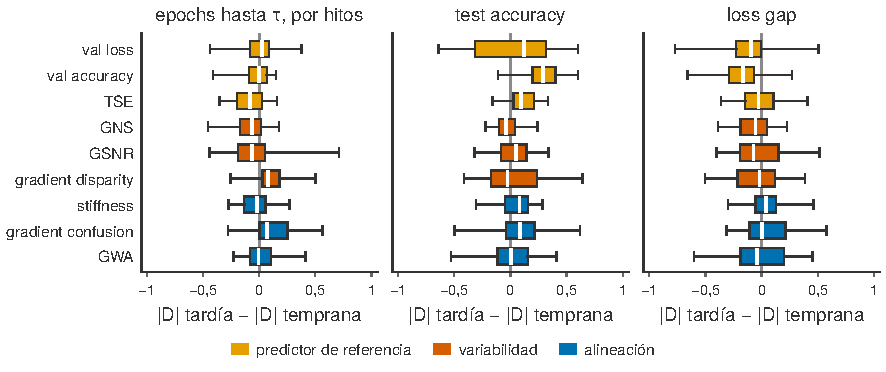
\includegraphics{ventanas}
\caption{Cambio de $|D|$ por celda al esperar.}
\label{fig:ventanas}
\end{figure}

Sobre el \emph{accuracy} de test, las seis métricas de gradiente no ganan nada esperando. Con el intervalo, la que más crece es la \emph{gradient disparity}, en seis celdas, y ninguna decrece en más de cuatro. Los recuentos crudos se reparten cerca de la mitad, entre 7 y 16 celdas que crecen de 24. Las medianas de $|D|$ van de 0,18 a 0,34 al 5\,\% y de 0,21 a 0,35 al 50\,\%. La que más sube es la \emph{gradient confusion}, de 0,18 a 0,29, con 16 celdas en crudo y cinco con intervalo. La \emph{stiffness} crece en 15 celdas en crudo y en cuatro con intervalo. Lo que sí crece es el predictor de referencia. El \emph{accuracy} de validación pasa de 0,40 a 0,70, con 22 celdas que crecen y 16 con intervalo, y TSE de 0,33 a 0,50, con 18 y 13. A mitad del entrenamiento la curva de validación ya es casi el resultado que se quiere predecir, y por eso su D crece. La Figura~\ref{fig:ventanas} lo enseña de un vistazo. En el panel del \emph{accuracy} de test, las cajas del \emph{accuracy} de validación y de TSE quedan a la derecha del cero, y las cajas de las seis métricas quedan centradas sobre él. La comparación de H2 repetida al 50\,\% dice lo mismo. En esa ventana ninguna métrica supera a la validación en más de dos celdas, y GWA pierde en 23, frente a las 13 del 5\,\%.

Sobre el \emph{gap} de \emph{loss} ocurre lo contrario con el predictor de referencia. El \emph{accuracy} de validación pierde $|D|$ al esperar, de 0,53 a 0,33, con 20 celdas que decrecen y ocho con intervalo, y el \emph{loss} de validación baja de 0,54 a 0,42. A presupuesto fijo el \emph{gap} es en buena parte velocidad leída al revés, según la Sección~\ref{sec:variables}, y la lectura temprana de la validación es la que mejor la recoge. Las métricas se reparten otra vez cerca de la mitad. Solo la \emph{stiffness} y la \emph{gradient confusion} crecen algo, de 0,39 a 0,51 y de 0,31 a 0,41, con cinco y cuatro celdas con intervalo. TSE es el único predictor que supera con claridad al \emph{loss} de validación al 50\,\%, con 16 celdas frente a ocho y nueve con intervalo, y sigue sin costar nada. El \emph{gap} de \emph{accuracy}, la lectura de apoyo, no cambia el cuadro, porque ninguna métrica crece con intervalo en más de cinco celdas.

Sobre la velocidad, entre la primera y la segunda ventana, casi nada se mueve con intervalo. Cada predictor cambia con intervalo en dos celdas como mucho, y las poblaciones en riesgo bajan hasta ocho entrenamientos en la segunda ventana. Los dos recuentos crudos que destacan son la \emph{gradient disparity}, que crece en 19 celdas y pasa de 0,28 a 0,44, y la \emph{gradient confusion}, que crece en 17. El resto se queda donde estaba. Las dos lecturas de la validación se quedan entre 0,69 y 0,74 en las dos ventanas, y TSE baja de 0,64 a 0,59.

H4 se sostiene para las métricas de gradiente, y por la razón menos favorable. Medir al 5\,\% predice tan bien como medir al 50\,\% porque su $|D|$ no crece con la ventana en la mayoría de las celdas con intervalo. Sobre el \emph{accuracy} de test, cuatro de las seis métricas se quedan planas, con medianas entre 0,2 y 0,35 en las dos ventanas. La \emph{stiffness} y la \emph{gradient confusion} crecen algo con el \emph{gap}, hasta 0,51 y 0,41, sin pasar de cinco celdas con intervalo. Ninguna se acerca a la validación, que sube hasta 0,70 con el \emph{accuracy} de test sin costar nada. La ventana mínima defendible es, por tanto, la primera, la \emph{epoch} 1 en MNIST y la 2 en los demás conjuntos. Lo es porque cuatro métricas no maduran y dos maduran poco, y esperar no cambia lo que dicen. Si bastaría medir antes no lo puede decir esta matriz, porque no tiene ninguna lectura anterior.

\section{Robustez entre optimizadores}
\label{sec:res-robustez}
% Fase F, escrita el 2026-09-04. Números de results/optimizadores.parquet (2026-09-04),
% regenerable con `uv run python src/contrast.py`. Sin figura: las inversiones van de 0 a 2.

Esta sección responde a la hipótesis H5 con la regla de la Sección~\ref{sec:protocolo-objetivos}. Las 24 celdas forman 12 pares. Las dos celdas de un par comparten conjunto de datos y arquitectura y solo difieren en el optimizador. El diseño las hizo comparables a propósito, con las mismas cinco \emph{seeds}, un umbral compartido y una rejilla de la misma forma, la de Adam la de SGD dividida entre 10. Para cada predictor y variable de la familia primaria se hacen tres recuentos sobre los 12 pares. El primero cuenta los pares que conservan el signo de la D y el segundo los que lo invierten. En los dos solo entran los pares en los que las dos D dejan fuera el cero por su intervalo, porque dos signos que coinciden sin intervalo coinciden por azar la mitad de las veces. Un par en el que alguna de las dos D incluye el cero no cuenta a ningún lado. El tercero cuenta los pares en los que la diferencia entre la D con SGD y la D con Adam deja fuera el cero. Como las dos D salen de entrenamientos distintos, ese intervalo suma las dos varianzas. Este recuento recoge los cambios de tamaño que no llegan a cambiar el signo. La Tabla~\ref{tab:h5} da los tres recuentos, como ac./inv. y dif., y la mediana del valor absoluto de D en cada brazo, como SGD/Adam.

\begin{table}[ht]
\centering
\footnotesize
\setlength{\tabcolsep}{2.5pt}
\caption{H5 sobre los 12 pares de celdas, $|D|$ con SGD y con Adam. En negrita, las inversiones.}
\label{tab:h5}
\begin{tabular}{lccccccccc}
\toprule
& \multicolumn{3}{c}{\textbf{\emph{Epochs} hasta el umbral}} & \multicolumn{3}{c}{\textbf{\emph{Accuracy} de test}} & \multicolumn{3}{c}{\textbf{\emph{Gap} de \emph{loss}}} \\
\cmidrule(lr){2-4}\cmidrule(lr){5-7}\cmidrule(lr){8-10}
\textbf{Predictor} & ac./inv. & dif. & SGD/Adam & ac./inv. & dif. & SGD/Adam & ac./inv. & dif. & SGD/Adam \\
\midrule
Posición en la rejilla & 1/\textbf{1} & 6 & 0,30/0,36 & 2/\textbf{2} & 6 & 0,42/0,18 & 4/0 & 3 & 0,51/0,40 \\
\addlinespace
\emph{Loss} de validación & 12/0 & 3 & 0,69/0,78 & 7/0 & 5 & 0,38/0,39 & 10/0 & 5 & 0,61/0,45 \\
\emph{Accuracy} de validación & 12/0 & 3 & 0,63/0,77 & 6/0 & 4 & 0,42/0,38 & 10/0 & 7 & 0,62/0,46 \\
TSE & 11/0 & 3 & 0,58/0,73 & 6/0 & 5 & 0,28/0,36 & 11/0 & 6 & 0,56/0,51 \\
\addlinespace
GNS & 4/0 & 0 & 0,27/0,30 & 3/0 & 0 & 0,23/0,22 & 1/\textbf{1} & 3 & 0,26/0,16 \\
GSNR & 5/0 & 1 & 0,27/0,35 & 4/0 & 0 & 0,20/0,28 & 4/0 & 5 & 0,25/0,33 \\
\emph{Gradient disparity} & 3/\textbf{1} & 4 & 0,48/0,23 & 5/\textbf{2} & 4 & 0,34/0,30 & 4/\textbf{2} & 5 & 0,37/0,31 \\
\addlinespace
\emph{Stiffness} & 3/\textbf{1} & 3 & 0,43/0,29 & 2/\textbf{1} & 4 & 0,25/0,15 & 5/0 & 2 & 0,21/0,43 \\
\emph{Gradient confusion} & 1/0 & 1 & 0,21/0,27 & 2/0 & 2 & 0,18/0,18 & 4/0 & 2 & 0,35/0,29 \\
GWA & 6/0 & 2 & 0,37/0,45 & 6/0 & 4 & 0,27/0,29 & 3/0 & 3 & 0,19/0,30 \\
\bottomrule
\end{tabular}
\end{table}

Ninguna métrica invierte el signo en más de dos pares de doce. La \emph{gradient disparity} invierte uno con la velocidad y dos con el \emph{accuracy} de test y con el \emph{gap}. La \emph{stiffness} invierte uno con la velocidad y uno con el \emph{accuracy} de test, y la escala de ruido uno con el \emph{gap}. GSNR, la \emph{gradient confusion} y GWA no invierten ninguno. Las inversiones de una misma métrica se concentran en pocos pares. Las de la disparidad con la velocidad y con el \emph{accuracy} de test caen en el mismo par, la red \emph{fully connected} sobre CIFAR-10. La segunda del \emph{accuracy} de test es la ResNet-18 sobre MNIST, y las dos del \emph{gap} son las redes convolucionales sobre CIFAR-100 y sobre Tiny-ImageNet. Las dos de la \emph{stiffness} caen en un solo par, la ResNet-18 sobre CIFAR-100. En esos pares la métrica cambia de sentido con las dos variables a la vez. Eso es lo que hace una métrica que lee el \emph{learning rate} cuando el mejor \emph{learning rate} de la rejilla queda a un lado con SGD y al otro con Adam. La posición en la rejilla lo muestra sola, con sus tres inversiones en MNIST. Los pares que acuerdan con intervalo son pocos para las métricas, entre uno y seis de doce. GWA es la que más acuerda en velocidad y en \emph{accuracy} de test, con seis pares en las dos, y la \emph{stiffness} en el \emph{gap}, con cinco. En el resto de pares una de las dos D incluye el cero y el par no cuenta. Las lecturas del predictor de referencia acuerdan en 11 o 12 pares con la velocidad, en seis o siete con el \emph{accuracy} de test y en 10 u 11 con el \emph{gap}, sin ninguna inversión.

Lo que sí cambia entre optimizadores es el tamaño de la asociación. La \emph{gradient disparity} pasa de una mediana de $|D|$ de 0,48 con SGD a 0,23 con Adam en velocidad, con cuatro pares en los que la diferencia deja fuera el cero. La \emph{stiffness} sube de 0,21 a 0,43 en el \emph{gap}. La posición en la rejilla baja de 0,42 a 0,18 con el \emph{accuracy} de test, con seis diferencias fuera del cero. Las lecturas del predictor de referencia son más fuertes con Adam en velocidad, entre 0,73 y 0,78 frente a entre 0,58 y 0,69, y más fuertes con SGD en el \emph{gap}, entre 0,56 y 0,62 frente a entre 0,45 y 0,51. Esas diferencias se leen primero como diferencias de población y solo después como efecto del optimizador. Los 41 entrenamientos divergidos son todos de SGD, y Adam no divergió en ninguno de sus 480. La norma del umbral de la Sección~\ref{sec:calibracion} se calculó sobre los dos optimizadores juntos, y la censura de la velocidad no es la misma en los dos brazos de un par.

H5 no se refuta y no queda demostrada. Con 12 pares, y entre uno y seis pares con las dos D fuera del cero por métrica, ninguna asociación segura cambia de signo en más de dos pares. Las inversiones que hay llegan de dos en dos, con las dos variables de un mismo par, con la forma de una métrica que lee el \emph{learning rate}. Este diseño no puede afirmar invariancia, porque 12 pares solo detectan inversiones groseras, y no encontrarlas no prueba que no las haya. Lo que sí se puede decir es que, allí donde una métrica ordena con seguridad bajo los dos optimizadores, ordena en el mismo sentido, y que el tamaño de esa ordenación cambia con el optimizador más de lo que cambia su signo.

\section{Concordancia con la literatura}
\label{sec:res-concordancia}
% Fase G, escrita el 2026-09-04 (H6, obj. \ref{obj:concordancia}). Números de results/signos.parquet
% (2026-09-04), regenerable con `uv run python src/contrast.py`; las predicciones son contrast.PREDICTED,
% la tabla de signos del vault por variable. Sin figura: son recuentos. La interpretación vive en Conclusiones.

Esta sección responde a la hipótesis H6 con la regla de la Sección~\ref{sec:protocolo-objetivos}. El artículo que propuso cada métrica predice el sentido de su relación con alguna variable, y la Sección~\ref{sec:hipotesis} fija esas predicciones. Para cada una se cuentan, sobre las 24 celdas de la familia primaria, las celdas con asociación del signo predicho y las celdas con asociación del signo contrario. El criterio de celda es el mismo intervalo de dos colas de las secciones anteriores, sin bajar la barra, y una celda significa lo mismo en todo el capítulo. No se calcula nada nuevo, porque las cifras son las de la Tabla~\ref{tab:signos-h1} partidas por el signo que cada artículo afirma. Entran siete predicciones de seis métricas. La \emph{stiffness} intra-clase y la \emph{gradient confusion} tienen predicción sobre la velocidad. La escala de ruido la tiene sobre la velocidad, donde coinciden la predicción de McCandlish et al. y la de la m-coherencia leída con el signo cambiado por la Ecuación~\ref{eq:gns-mcoh}, y sobre el \emph{gap}, donde la única predicción es la de la m-coherencia. GSNR la tiene sobre el \emph{gap}. La \emph{gradient disparity} la tiene sobre el \emph{accuracy} de test, porque su artículo la liga al error de test. GWA la tiene sobre el \emph{accuracy} de test, con el signo convertido de la Sección~\ref{sec:def-alineacion}. Las cinco predicciones que esta memoria extrapola de un artículo a otra variable ocupan la segunda mitad de la Tabla~\ref{tab:h6} y quedan fuera del veredicto. La tabla repite la cuenta dentro de cada arquitectura, porque la Sección~\ref{sec:res-familia} mostró que el signo cambia con ella. En negrita van las cuentas en contra que superan a las cuentas a favor.

\begin{table}[ht]
\centering
\footnotesize
\setlength{\tabcolsep}{3.5pt}
\caption{H6 al 5\,\%, sobre las 24 celdas y dentro de cada arquitectura. En negrita, las cuentas en contra que superan a las de a favor.}
\label{tab:h6}
\begin{tabular}{llllcccc}
\toprule
\textbf{Predictor} & \textbf{Variable} & \textbf{Base} & \textbf{Signo} & \textbf{Celdas} & \textbf{FC} & \textbf{CNN} & \textbf{ResNet-18} \\
\midrule
\multicolumn{8}{l}{\textbf{Predicciones que el artículo enuncia}} \\
\emph{Stiffness} & Velocidad & Fort et al.~\cite{fort2019stiffness} & $-$ & 5/\textbf{9} & 1/2 & 0/4 & 4/3 \\
\emph{Gradient confusion} & Velocidad & Sankararaman et al.~\cite{sankararaman2020impact} & $+$ & 5/4 & 4/0 & 0/3 & 1/1 \\
GNS & Velocidad & McCandlish et al.~\cite{mccandlish2018empirical} & $+$ & 7/3 & 0/1 & 2/0 & 5/2 \\
 & & y Chatterjee~\cite{chatterjee2020coherent} & & & & & \\
GNS & \emph{Gap} & Chatterjee y Zielinski~\cite{chatterjee2020making} & $+$ & 5/\textbf{6} & 0/2 & 1/3 & 4/1 \\
GSNR & \emph{Gap} & Liu et al.~\cite{liu2020understanding} & $-$ & 11/2 & 4/2 & 3/0 & 4/0 \\
\emph{Gradient disparity} & \emph{Accuracy} & Forouzesh y Thiran~\cite{forouzesh2021disparity} & $-$ & 4/\textbf{12} & 2/5 & 0/6 & 2/1 \\
GWA & \emph{Accuracy} & Hölzl et al.~\cite{hoelzl2025gradient} & $-$ & 15/1 & 7/0 & 3/0 & 5/1 \\
\addlinespace
\multicolumn{8}{l}{\textbf{Predicciones que esta memoria extrapola, sin contrastar}} \\
\emph{Gradient disparity} & Velocidad & del error de test & $+$ & 4/\textbf{9} & 2/5 & 0/4 & 2/0 \\
GSNR & Velocidad & del \emph{gap} & $-$ & 7/6 & 1/0 & 0/5 & 6/1 \\
GSNR & \emph{Accuracy} & del \emph{gap} & $+$ & 7/4 & 3/0 & 0/4 & 4/0 \\
GWA & Velocidad & del \emph{accuracy} de test & $+$ & 16/1 & 7/0 & 4/0 & 5/1 \\
GWA & \emph{Gap} & del \emph{accuracy} de test & $+$ & 6/4 & 0/0 & 0/4 & 6/0 \\
\bottomrule
\end{tabular}
\end{table}

Dos de las tres predicciones sobre el desenlace final se cumplen. GWA con el \emph{accuracy} de test va en el sentido de su artículo en 15 celdas y en contra en una, la ResNet-18 sobre Tiny-ImageNet con SGD. Lo hace en las tres arquitecturas, con siete de las ocho celdas de la red \emph{fully connected}. GSNR con el \emph{gap} va a favor en 11 celdas y en contra en dos, las dos de la red \emph{fully connected} sobre CIFAR-10, también en las tres arquitecturas. La tercera va en contra. El artículo de la \emph{gradient disparity} la liga a un error de test mayor. Aquí una disparidad alta acompaña a un \emph{accuracy} de test mayor en 12 celdas, las seis de la convolucional, cinco de la red \emph{fully connected} y una de la ResNet-18, frente a cuatro en el sentido del artículo. Las tres predicciones sobre la velocidad apenas reciben apoyo. La escala de ruido va a favor en siete celdas y en contra en tres, las tres en MNIST, y la sostiene la ResNet-18 con cinco de las siete. La \emph{gradient confusion} da cinco celdas a favor y cuatro en contra, y las dos cuentas no se mezclan, porque las cuatro de la red \emph{fully connected} van con su artículo y las tres de la convolucional en contra. La \emph{stiffness} va en contra, con nueve celdas frente a cinco. La convolucional la contradice en sus cuatro celdas con asociación, y la ResNet-18 la apoya en cuatro y la contradice en tres. La predicción de la m-coherencia sobre el \emph{gap}, leída sobre la escala de ruido, da cinco celdas a favor y seis en contra.

Donde el signo contradice al artículo, la Sección~\ref{sec:protocolo-objetivos} pide leer primero la composición de dos curvas sobre el \emph{learning rate}, y las dos discrepancias tienen esa forma. El artículo de la \emph{stiffness} fijó su signo a lo largo del tiempo de entrenamiento, con la \emph{stiffness} cayendo hacia cero al entrar en el sobreajuste. Aquí, dentro de la celda, la \emph{stiffness} del 5\,\% ordena los entrenamientos al revés que el \emph{accuracy} de validación de esa misma ventana, con una D de mediana $-0{,}44$ según la Sección~\ref{sec:res-por-condicion}. El entrenamiento que más ha avanzado en la ventana tiene los gradientes de una misma clase menos alineados, y es el que cruza el umbral antes. Una \emph{stiffness} alta marca, por tanto, a un entrenamiento retrasado por su \emph{learning rate}, y esa cuenta no pone a prueba el mecanismo del artículo. La \emph{gradient disparity} es el mismo caso con el signo contrario. Su artículo la vio crecer con el sobreajuste y con el ruido de etiquetas. Aquí ordena los entrenamientos como el \emph{accuracy} de validación de la ventana, con una D de mediana 0,26 y positiva en 16 celdas, porque las dos dibujan un pico a lo largo del \emph{learning rate}. Una disparidad alta marca al entrenamiento que más ha avanzado en la ventana, y el sobreajuste que su artículo describe es un eje que la celda no recorre. La \emph{gradient confusion}, cuyo artículo fijó el signo a lo largo de la anchura y la profundidad de la red, cambia de signo entre la red plana y la convolucional, con cuentas de cuatro y de tres celdas. Del lado de los acuerdos vale el aviso contrario. GWA coincide con su artículo casi sin excepción, pero ordena los entrenamientos en parte como el \emph{accuracy} de validación, con una D de mediana $-0{,}45$, y peor que él, según midió la Sección~\ref{sec:res-incremental}. La razón está en la Sección~\ref{sec:def-alineacion}. GWA es un margen normalizado que el paso hacia delante ya calcula casi por completo. Su acuerdo confirma al artículo en lo que el artículo mide, sin añadir una prueba independiente sobre los gradientes, porque no supera a la validación.

De las extrapoladas, GWA con la velocidad va en el sentido extrapolado en 16 celdas y en contra en una, la misma ResNet-18 sobre Tiny-ImageNet con SGD. Es la lectura en velocidad de esa misma relación con la validación. GWA con el \emph{gap} se parte por arquitectura, con seis celdas a cero en la ResNet-18 en el sentido extrapolado y cero a cuatro en la convolucional, como recogió la Sección~\ref{sec:res-familia}. GSNR con la velocidad da siete celdas contra seis, con la convolucional en contra en cinco y la ResNet-18 a favor en seis, y con el \emph{accuracy} de test siete contra cuatro. La \emph{gradient disparity} con la velocidad va en contra de la extrapolación, con cuatro celdas frente a nueve. Una relación que un artículo sugiere y que no se registró como predicción se reporta solo como observación. La \emph{stiffness}, cuyo artículo la presenta como una perspectiva sobre la generalización, muestra asociación negativa con el \emph{gap} en 15 celdas y positiva en una, el sentido que ese título sugiere. No entra en el veredicto, porque una predicción registrada después de ver el signo no contrasta nada.

H6 cae en parte. De las siete predicciones, dos se cumplen en las tres arquitecturas, GWA con el \emph{accuracy} de test y GSNR con el \emph{gap}. Tres no reciben apoyo, la \emph{gradient confusion} y la escala de ruido con la velocidad y la m-coherencia con el \emph{gap}, con entre cinco y siete celdas a favor de 24 y casi tantas en contra. Dos van sistemáticamente en contra, la \emph{stiffness} con la velocidad, con nueve celdas frente a cinco, y la \emph{gradient disparity} con el \emph{accuracy} de test, con 12 frente a cuatro, las dos con la forma que la composición de curvas anticipa. El reparto tiene lógica. Una métrica leída al 5\,\% describe el estado del entrenamiento en ese momento, y ese estado anticipa dónde acaba el entrenamiento, igual que lo anticipa el \emph{accuracy} de validación. Un artículo que fijó su signo a lo largo del tiempo o del ruido de etiquetas predice otra cosa, y dentro de la celda esa lectura se confunde con el \emph{learning rate}. Lo que H6 sostiene es, por tanto, más estrecho que su enunciado. Los signos se reproducen donde el artículo habla del desenlace y la métrica describe ese desenlace, GWA y GSNR, y se invierten donde el artículo fijó el signo sobre un eje que esta matriz no recorre. Reproducirlos no convierte a ninguna métrica en una señal que supere a la validación, según decidió la Sección~\ref{sec:res-incremental}.

\section{Conclusiones del capítulo}
\label{sec:res-conclusiones}

Los datos sirven para la pregunta, con cinco salvedades medidas. La censura de la velocidad es consecuencia del diseño, y contada en pares comparables cada celda conserva entre el 62 y el 99\,\% de los suyos. El \emph{learning rate} explica entre el 45 y el 92\,\% de la dispersión de las seis métricas dentro de la celda, según la mediana sobre las 24 celdas. En las tres lecturas del predictor de referencia explica el 95\,\% o más. Toda D lleva dentro, por tanto, esa causa común. Para la velocidad solo predicen las dos primeras ventanas, y el mejor \emph{loss} de validación deja de predecir al 25\,\% en 15 celdas, por el sobreajuste. La curva de validación cuenta lo mismo que el test, en orden y en nivel. El \emph{batch} de medición de 256 ejemplos deja al estimador de la escala de ruido cerca de su valor de referencia de 255, y al 5\,\% más de un tercio de las lecturas de los entrenamientos que aprendieron queda por encima de 200. Ahí el estimador ya no resuelve las escalas de $10^{3}$ a $10^{4}$ que McCandlish et al. reportan, según deriva la Sección~\ref{sec:def-variabilidad}, y conserva el orden dentro de la celda con menos potencia.

Los seis veredictos, sobre la familia primaria al 5\,\% y los 806 entrenamientos que aprendieron, son estos. H1 se sostiene como requisito previo, porque GWA muestra asociación del mismo signo con la velocidad en 16 celdas y con el \emph{accuracy} de test en 15, más que la posición en la rejilla, y la cuenta granulada queda vacía. H2 cae, porque ninguna métrica supera a la validación de la misma ventana con intervalo ni elige mejor el \emph{learning rate}, y GWA cuesta 0,023 de \emph{accuracy} frente a 0,013. H3 cae, porque la alineación pone la primera métrica y también la última, y el orden cambia con la arquitectura. H4 se sostiene, porque cuatro métricas no maduran y dos maduran poco, mientras la validación sube hasta 0,70. H5 no se refuta ni queda demostrada, con entre cero y dos inversiones en 12 pares. H6 cae en parte, con dos predicciones cumplidas, tres sin apoyo y dos invertidas por la composición de curvas sobre el \emph{learning rate}. Ninguna clase de coste compra más capacidad predictiva que la clase gratuita.

La Tabla~\ref{tab:aportaciones} reúne, métrica a métrica, lo que las secciones anteriores reparten por hipótesis, qué lee cada una, qué anticipa al 5\,\% y en cuántas celdas, dónde falla y cómo queda frente a su artículo y frente a la validación. Una D se traduce a pares, porque $(D + 1)/2$ es la parte de los pares comparables que el predictor ordena bien. La D de 0,40 de GWA con la velocidad son siete pares de cada diez, y la de 0,71 del \emph{accuracy} de validación, ocho y medio.

\begin{table}[htbp]
\centering
\scriptsize
\setlength{\tabcolsep}{3pt}
\caption{Qué anticipa cada métrica al 5\,\%, sobre las 24 celdas y los 806 entrenamientos que aprendieron.}
\label{tab:aportaciones}
\begin{tabular}{>{\raggedright\arraybackslash}p{1.9cm}
                >{\raggedright\arraybackslash}p{2.5cm}
                >{\raggedright\arraybackslash}p{3.5cm}
                >{\raggedright\arraybackslash}p{3.0cm}
                >{\raggedright\arraybackslash}p{2.9cm}}
\toprule
\textbf{Métrica} & \textbf{Qué lee} & \textbf{Qué anticipa, celdas a favor y en contra} & \textbf{Dónde falla} & \textbf{Frente al artículo y a la validación} \\
\midrule
GWA\newline alineación; barrido, lineal & Coseno entre el gradiente y los pesos de la última capa, un margen normalizado por ejemplo & Alta, cruce más tardío (16/1) y menos \emph{accuracy} de test (15/1), en los cuatro conjuntos y las tres arquitecturas. Con el \emph{gap}, nada (6/4) & Una celda al revés, la ResNet-18 sobre Tiny-ImageNet con SGD. Con el \emph{gap} cambia de signo entre la convolucional y la ResNet-18 & Signo del artículo, 15/1. Pierde con la validación con intervalo en ocho celdas, sin ganar en ninguna; elegir con ella cuesta 0,023 frente a 0,013 \\
\addlinespace[2pt]
\emph{Stiffness}\newline alineación; barrido, cuadrática & Coseno medio entre gradientes de ejemplos de la misma clase & Alta, \emph{gap} menor (15/1), tantas celdas como la posición en la rejilla (15/0), y cruce más tardío (9/5) & La ResNet-18 se parte con el \emph{gap}; con 100 y 200 clases descansa en menos del 1\,\% de los pares; con Adam dobla su asociación con el \emph{gap} & Al revés que su artículo en velocidad (5/9). Pierde con el \emph{loss} de validación 7/17; elegir con ella cuesta 0,110, más que el azar \\
\addlinespace[2pt]
\emph{Gradient disparity}\newline variabilidad; cinco pasadas propias & Distancia entre los gradientes de dos submuestras, la raíz de la traza de la covarianza del ruido & Alta, más \emph{accuracy} de test (12/4) y \emph{gap} menor (11/4); segunda en las tres variables & Se da la vuelta en MNIST y en la ResNet-18; con Adam ordena la velocidad la mitad de fuerte que con SGD; la que más invierte entre optimizadores, cinco inversiones de 36 & Al revés que su artículo con el test (4/12). Gana a la validación con intervalo en tres celdas y pierde en ocho; cuesta 0,097 con el signo del artículo \\
\addlinespace[2pt]
GSNR\newline variabilidad; barrido, lineal & Razón señal-ruido del gradiente, parámetro a parámetro & Alto, \emph{gap} menor (11/2), en las tres arquitecturas & Con la velocidad y el test cambia de bando entre la convolucional, en contra, y la ResNet-18, a favor & Signo del artículo con el \emph{gap}, 11/2. Pierde con el \emph{loss} de validación 5/19; cuesta 0,035, la segunda mejor \\
\addlinespace[2pt]
Escala de ruido\newline variabilidad; barrido, lineal & Traza de la covarianza sobre la norma del gradiente medio, la m-coherencia con otro nombre & Nada con claridad, velocidad 7/3, test 3/6 y \emph{gap} 5/6 & La sostiene solo la ResNet-18 en velocidad, con las tres celdas en contra en MNIST; contra el techo del estimador en un tercio de las lecturas & Su artículo, 7/3 sin apoyo claro; la m-coherencia con el \emph{gap}, 5/6. Pierde con la validación 6/18; cuesta 0,073, más que el azar \\
\addlinespace[2pt]
\emph{Gradient confusion}\newline alineación; barrido, cuadrática & El coseno más negativo entre pares de ejemplos & Nada con claridad, velocidad 5/4, test 5/5 y \emph{gap} 9/5; la que más crece al esperar, de 0,18 a 0,29 con el test & Cambia de bando con la velocidad entre la red plana (4/0) y la convolucional (0/3) & Su artículo, 5/4 sin apoyo. Pierde con la validación 6/17; cuesta 0,059 \\
\bottomrule
\end{tabular}
\end{table}

\chapter{Conclusiones}
\label{ch:conclusiones}
% No es un resumen: interpreta. Una conclusión por objetivo. Se cierra tras Resultados.

\section{Cumplimiento de objetivos}
\label{sec:concl-objetivos}
% Repasar H1-H6; un resultado negativo robusto (H1 sí, H2 no) es contribución válida.
% Aquí vive la interpretación de los datos y el contraste con el estado del arte (\ref{ch:estado-del-arte});
% Resultados solo describe (guía ETSINF). Una conclusión parcial por objetivo.

\section{Aportaciones}
\label{sec:concl-aportaciones}
% Comparativa multi-familia, barrido temporal, coste asintótico frente a capacidad predictiva.

\section{Limitaciones}
\label{sec:concl-limitaciones}
% Solo visión, correlacional, sin augmentation. El barrido por ejemplo recorre todos los parámetros en las tres redes; solo GWA lee la última capa.
% Las líneas de continuación viven ahora en su propio capítulo, \ref{ch:trabajos-futuros}.

\chapter{Trabajos futuros}
\label{ch:trabajos-futuros}
% Capítulo aparte por indicación de los seminarios ETSINF. Va tras Conclusiones.
% Fuera del rango 2-6, así que no lleva hoja de ruta formal ni sección de conclusiones,
% igual que la Introducción y las Conclusiones.
% El régimen post-meseta se cuenta en cualitativo a propósito: los porcentajes viven en
% reports_pilot/, que está en .gitignore y solo existe en el disco local.

Este capítulo recoge lo que el trabajo deja abierto. Actuar sobre la señal en lugar de limitarse a medirla es el paso que la pregunta de investigación no aborda, y es la continuación que la Sección~\ref{sec:alcance} anuncia al declarar el alcance. Ampliar ese alcance por los ejes que la matriz congeló a propósito es la segunda vía. La tercera la forman las deudas de medición que el propio diseño reconoce y que los datos disponibles no pueden saldar.

\section{Intervención sobre la señal}
\label{sec:futuro-intervencion}

El diseño de este trabajo es correlacional. Mide si una métrica temprana anticipa la eficiencia, no si actuar sobre ella durante el entrenamiento sirve de algo. La continuación evidente es dar ese salto y usar la métrica para decidir en marcha, deteniendo un entrenamiento que no va a compensar o ajustando el \emph{learning rate} en función de lo medido.

El salto exige dos cosas que aquí no existen. La primera es un criterio de decisión, esto es, un valor de la métrica a partir del cual se actúa y una regla de qué hacer entonces, y ese criterio depende de lo que responda H2. Si ninguna métrica supera al predictor de referencia, la intervención se construiría igual de bien sobre la curva de \emph{loss}, sin calcular ningún gradiente, y el coste de instrumentación no tendría justificación.

La segunda es un diseño experimental propio. Una intervención altera el entrenamiento que observa, porque en cuanto se detiene una ejecución o se cambia su \emph{learning rate} a partir de la métrica, la trayectoria deja de ser la que aquí se ha medido. Los 960 entrenamientos de esta matriz no se pueden reanalizar para responder esa pregunta, de modo que haría falta una matriz nueva con la intervención dentro del bucle.

\section{Extensión del alcance}
\label{sec:futuro-alcance}

El estudio se limita a clasificación de imágenes, y deja fuera los demás dominios y las arquitecturas de tipo \emph{transformer}. Nada en la definición de las ocho métricas las ata a la visión, porque todas se construyen sobre el gradiente por ejemplo y ese objeto existe en cualquier red entrenada por descenso de gradiente. Lo que queda por saber es si la asociación sobrevive al cambio de dominio, que es una pregunta empírica y no de definición.

El conjunto ImageNet completo se sustituyó por Tiny-ImageNet por restricciones de disco y de cómputo. El conjunto de datos es uno de los dos ejes que más mueven el nivel de eficiencia, según recoge la Sección~\ref{sec:riesgos}, así que llevar el estudio a un conjunto verdaderamente grande comprobaría la relación justo donde predecir la eficiencia sale más caro y, por tanto, más rentable.

El entrenamiento se hizo sin \emph{data augmentation} para no añadir una fuente de azar al proceso. Recuperarlo no es solo entrenar en condiciones más habituales, porque el \emph{batch} de medición se extrae del conjunto de entrenamiento con la misma transformación y pasaría a estar formado por versiones distorsionadas de los ejemplos. Medir con \emph{data augmentation} es, entonces, medir otra cosa, y comprobar cuánto cambian los valores sería un resultado por sí mismo.

La partición entre entrenamiento y validación es fija y compartida por los 960 entrenamientos. Aleatorizarla mediría también cuánto varía el estimador frente al reparto de los datos, que la Sección~\ref{sec:protocolo-eval} declara pregunta legítima pero distinta de la que aquí se formula.

\section{Medición y métricas}
\label{sec:futuro-medicion}

Tres deudas de medición quedan reconocidas en el texto y sin saldar. La variante de signo de la \emph{stiffness} es la más informativa entre clases distintas, pero exige una muestra mayor que la de un \emph{batch} de medición barato para no quedar dominada por el ruido, y agrandarlo encarece de forma cuadrática el recorrido de todos los pares. Estudiarla pide, por tanto, un protocolo menos restrictivo que el de esta matriz.

La versión exacta de la escala de ruido del gradiente se descartó por coste, porque requiere la Hessiana, y en su lugar se emplea la forma simplificada, que supone la curvatura proporcional a la identidad. Ese supuesto es cómodo pero no inocuo, y medir cuánto se separan las dos versiones sobre unas pocas configuraciones diría qué se está perdiendo al aceptarlo.

El presupuesto de \emph{epochs} se calibró donde el \emph{loss} de validación se aplana, y las métricas de alineación siguen evolucionando después de esa meseta mientras el \emph{accuracy} ya no mejora, según se observó en las trayectorias extendidas del piloto de calibración. La matriz corta en el presupuesto, de manera que observa las métricas en fase transitoria y no puede decir nada del régimen posterior. Caracterizarlo exigiría entrenamientos más largos, y la evidencia del piloto es de una sola ejecución por celda y solo descriptiva.

Queda por último el coste, que este trabajo acota en notación asintótica pero no mide por métrica. El barrido compartido calcula los gradientes por ejemplo una sola vez y los reparte entre las seis métricas que los consumen, y el resumen de cada entrenamiento guarda un único reloj de instrumentación, así que el coste marginal de una métrica concreta no se puede recuperar ni siquiera a posteriori. Obtenerlo pide un banco de pruebas aparte, de minutos y fuera de la matriz, que cronometre cada métrica por separado sobre las mismas redes. En la dirección contraria, los datos ya guardan el tiempo de reloj hasta el umbral, que este trabajo registra sin declararlo variable del estudio. Es la lectura de velocidad pertinente al comparar SGD con Adam, porque su paso no cuesta lo mismo, y explotarla no exigiría ningún entrenamiento nuevo.


\printbibliography[heading=bibintoc]
\cleardoublepage

\APPENDIX
\chapter{Objetivos de Desarrollo Sostenible}
\label{ap:ods}
% Anexo obligatorio desde las convocatorias de 2022. Reproduce la plantilla oficial de la
% ETSINF: tabla de los 17 ODS y reflexión de 500 a 1.500 palabras. El mismo texto va en
% thesis/anexo-ods.docx, el fichero suelto que se sube a Ebrón con el depósito.

\section{Grado de relación del trabajo con los ODS}
\label{sec:ods-tabla}

La Tabla~\ref{tab:ods} sitúa este trabajo frente a cada uno de los 17 Objetivos de Desarrollo Sostenible de la Agenda 2030, en los cuatro niveles que fija la plantilla de la escuela. Ningún objetivo alcanza el nivel alto, porque el trabajo no actúa directamente sobre ningún problema social ni ambiental. Tres quedan en el nivel medio, los relativos a la energía, a la innovación y al consumo responsable, y dos en el nivel bajo, la educación y la acción por el clima. La Sección~\ref{sec:ods-reflexion} justifica cada uno.

\begin{table}[htbp]
  \centering
  \caption{Relación del trabajo con los 17 ODS.}
  \label{tab:ods}
  \begin{tabular}{>{\raggedright\arraybackslash}p{8cm}cccc}
    \toprule
    Objetivos de Desarrollo Sostenible & Alto & Medio & Bajo & No procede \\
    \midrule
    1. Fin de la pobreza & & & & $\times$ \\
    2. Hambre cero & & & & $\times$ \\
    3. Salud y bienestar & & & & $\times$ \\
    4. Educación de calidad & & & $\times$ & \\
    5. Igualdad de género & & & & $\times$ \\
    6. Agua limpia y saneamiento & & & & $\times$ \\
    7. Energía asequible y no contaminante & & $\times$ & & \\
    8. Trabajo decente y crecimiento económico & & & & $\times$ \\
    9. Industria, innovación e infraestructuras & & $\times$ & & \\
    10. Reducción de las desigualdades & & & & $\times$ \\
    11. Ciudades y comunidades sostenibles & & & & $\times$ \\
    12. Producción y consumo responsables & & $\times$ & & \\
    13. Acción por el clima & & & $\times$ & \\
    14. Vida submarina & & & & $\times$ \\
    15. Vida de ecosistemas terrestres & & & & $\times$ \\
    16. Paz, justicia e instituciones sólidas & & & & $\times$ \\
    17. Alianzas para lograr objetivos & & & & $\times$ \\
    \bottomrule
  \end{tabular}
\end{table}

\section{Reflexión}
\label{sec:ods-reflexion}

Entrenar una red neuronal profunda es hoy una de las operaciones más caras del aprendizaje automático, en tiempo de máquina, en energía y en dinero. La forma habitual de saber si una configuración merece la pena sigue siendo lanzarla entera y mirar el resultado al final, y buena parte del cómputo se gasta en entrenamientos que un observador con mejor información habría detenido pronto. Este trabajo estudia una de las señales que podrían aportar esa información, las métricas calculadas sobre los gradientes de la red durante su fracción temprana, y mide si predicen la eficiencia del entrenamiento completo. Es un estudio correlacional sobre 960 entrenamientos de clasificación de imágenes, y su relación con la Agenda 2030 pasa por el cómputo que ese tipo de entrenamiento consume.

La relación más directa es con el ODS 7, energía asequible y no contaminante, y a través de él con el ODS 13, acción por el clima. Un entrenamiento que no va a converger, o que va a hacerlo más despacio de lo que su presupuesto permite, consume la misma electricidad que uno bueno hasta que alguien lo detiene. Si una medida tomada en el primer 5\,\% del presupuesto anticipara ese desenlace, el resto de la energía podría ahorrarse, y la decisión de cortar dejaría de depender de la intuición de quien mira la curva. Esa es la promesa práctica del trabajo y también su límite, porque aquí solo se mide si la señal existe, y decidir a partir de ella queda para un estudio posterior. La relación con el objetivo se mantiene con una respuesta negativa, que es la que este trabajo obtuvo. Calcular las métricas de gradiente cuesta cómputo, en esta matriz 24,1 de las 121,7 horas totales. Ninguna de ellas superó a la información gratuita de la curva de validación en la primera ventana, así que el resultado dice a quien entrena que no gaste ese cómputo. Un resultado negativo bien medido evita un consumo tan real como el que evitaría un resultado positivo. El ODS 13 se queda en el nivel bajo porque el trabajo no mide emisiones ni energía, solo horas de una GPU, y cualquier conversión a kilovatios hora sería una estimación ajena a lo medido.

El ODS 12, producción y consumo responsables, recoge la manera en que se ha gastado el cómputo del propio estudio. La matriz se diseñó una sola vez, con el tamaño mínimo que la pregunta necesitaba, y se ejecutó en una única GPU a lo largo de 121,7 horas de reloj. Antes de lanzarla se hizo un piloto de calibración por celda para fijar el presupuesto de \emph{epochs} sobre curvas de entrenamiento reales. El lanzador guarda cada entrenamiento terminado y reanuda solo lo pendiente, así que ninguno se repitió por accidente. Los resultados completos, con los dos relojes de cada entrenamiento, el de aprendizaje y el de medición, están versionados junto al código, y cualquier lector puede reanalizarlos sin volver a entrenar nada. Declarar el coste entero de la instrumentación junto a su posible beneficio es la parte del consumo responsable que un estudio como este puede cumplir por sí mismo.

El ODS 9, industria, innovación e infraestructuras, pide reforzar la investigación científica y la capacidad tecnológica. Este trabajo aporta una pieza pequeña de esa capacidad, una comparación sistemática de ocho métricas ya publicadas contra un predictor de referencia que no cuesta nada, sobre una matriz común de conjuntos de datos, arquitecturas y optimizadores. Las métricas se propusieron en artículos distintos, cada uno con su propio banco de pruebas, y hasta ahora no se habían medido todas en las mismas condiciones. El código que las calcula, con sus pruebas unitarias, queda disponible para que otro grupo lo aplique a sus propios entrenamientos o lo extienda a dominios que aquí quedan fuera, como el texto o las arquitecturas de tipo \emph{transformer}. La relación se queda en el nivel medio porque la aportación es una evaluación de herramientas existentes y no una infraestructura nueva.

El ODS 4, educación de calidad, tiene una relación indirecta. La memoria documenta el diseño, las decisiones y los errores encontrados por el camino, y el repositorio guarda los datos, el código y las pruebas que permiten repetir el estudio de principio a fin. Ese material puede servir de ejemplo trabajado de un estudio empírico reproducible para estudiantes de ciencia de datos, y en esa medida el trabajo contribuye a la formación, aunque no se haya concebido como recurso docente. Por esa razón se marca en el nivel bajo.

Los 12 objetivos restantes no proceden. El trabajo no recoge datos nuevos y trabaja con cuatro conjuntos de datos públicos de imágenes, de uso general en la investigación. No toma ninguna decisión que afecte a personas, a la salud, a la alimentación, al agua, a las ciudades, a los ecosistemas o a las instituciones. Tampoco tiene una dimensión de género ni de reducción de desigualdades más allá de la que comparte cualquier trabajo que publica su código en abierto. Marcarlos como no procedentes es más honesto que forzar una relación que la memoria no puede sostener.

La Agenda 2030 pide a la ingeniería que gaste menos para conseguir lo mismo. En el aprendizaje automático, el gasto que más crece es el del entrenamiento, y saber pronto qué entrenamientos no compensan es una de las pocas vías de ahorro que no exige cambiar el modelo ni los datos. Este trabajo mide si la señal para esa decisión existe antes de que nadie la use, y encuentra que ninguna métrica de gradiente mejora a la más barata de todas, la curva de validación.

\chapter{Configuración del sistema y reproducibilidad}
\label{ap:configuracion}
% Fuente: uv.lock, src/seed.py, src/train.py, run_matrix.py, run_pilot.py, git log sobre
% reports/ y reports_pilot/, y los 960 summary.json. Cifras verificadas el 2026-09-03.
% Lo que Desarrollo ya cuenta (relojes, reanudación, semillas, normalización) no se repite:
% este apéndice da versiones, órdenes, máquina y alcance.

Este apéndice recoge lo que hace falta para repetir el estudio: las versiones del software, las órdenes que ejecutan los entrenamientos y los análisis, la máquina, y qué parte del resultado se reproduce en otra máquina.

\section{Entorno software}
\label{sec:entorno}

El código es Python, gestionado con \texttt{uv}; los entrenamientos y los análisis corrieron con la versión 3.12.8. Las dependencias están fijadas en \texttt{uv.lock}, y \texttt{uv sync} las instala en un entorno propio del proyecto. Las que intervienen en los cálculos son PyTorch 2.11.0 y torchvision 0.26.0, NumPy 2.4.4, pandas 3.0.3, PyArrow 24.0.0, Pillow 12.2.0, SciPy 1.18.0 y Matplotlib 3.11.0.

Los conjuntos de datos se descargan con \texttt{uv run python src/load\_data.py}, que deja MNIST, CIFAR-10 y CIFAR-100 bajo \texttt{data/}; Tiny-ImageNet hay que colocarlo a mano en \texttt{data/tiny-imagenet-200/}, con sus carpetas \texttt{train/} y \texttt{val/}. La matriz se ejecuta con \texttt{uv run python src/run\_matrix.py}, que con \texttt{--init} escribe los 24 ficheros de celda en \texttt{experiments/} y con \texttt{--status} cuenta los entrenamientos hechos y pendientes; el piloto, con \texttt{src/run\_pilot.py}, que se lee con \texttt{--report}; y un entrenamiento suelto, con \texttt{src/train.py} y las opciones \texttt{--config}, \texttt{--lr} y \texttt{--seed}. Los análisis se regeneran desde \texttt{reports/} con tres órdenes y la memoria con una cuarta:
\begin{itemize}
\item \texttt{uv run python src/efficiency.py} imprime los diagnósticos de las Secciones~\ref{sec:res-cobertura} a~\ref{sec:res-solape};
\item \texttt{uv run python src/contrast.py} calcula el contraste de la Sección~\ref{sec:protocolo-analisis} y escribe en \texttt{results/} las tablas \texttt{tabla\_larga.parquet}, \texttt{tabla\_larga\_960.parquet} y \texttt{seleccion.parquet};
\item \texttt{uv run python src/figures.py} dibuja las figuras en \texttt{thesis/img/};
\item \texttt{latexmk -pdf -r thesis/.latexmkrc -cd thesis/main.tex} compila la memoria en \texttt{thesis/render/}.
\end{itemize}
La batería de pruebas se ejecuta con \texttt{uv run pytest}.

\section{Hardware y ejecución}
\label{sec:hardware}

Los 960 entrenamientos y el piloto corrieron en una sola máquina con Linux y una GPU NVIDIA GeForce RTX 5080 de 16 GB, sin clúster ni ejecución en paralelo. La memoria del anfitrión importa tanto como la de la GPU, porque el barrido compartido de la Sección~\ref{sec:des-metricas} reúne en ella la matriz de gradientes por ejemplo para formar el Gram: con $M = 256$ son 14,2 GB para la red \emph{fully connected} sobre Tiny-ImageNet y 11,5 GB para la ResNet-18, además de lo que consume el propio entrenamiento.

Los 960 corrieron con el mismo código de medición, el del repositorio en \texttt{b38f635}: el primer entrenamiento se versionó el 8 de agosto de 2026 (\texttt{9fe77ab}) y el último el 22 (\texttt{f6df900}), sin ningún cambio entre esas fechas en el código de entrenamiento ni en las métricas. El 29 de agosto (\texttt{1ca5f65} y \texttt{a2e1ab8}) los signos de la \emph{stiffness} y la fracción negativa de la \emph{gradient confusion} pasaron a devolver NaN donde el valor es indefinido, en lugar de un cero, también en los datos ya guardados en \texttt{reports/}. Los 24 ficheros de \texttt{experiments/} conservan el umbral de junio porque el lanzador no sobrescribe un fichero existente; ningún cálculo los lee. El piloto son 24 entrenamientos en \texttt{reports\_pilot/} (\texttt{3b84f5b}), ejecutados con el código de junio, y sus seis resúmenes de Tiny-ImageNet llevan la clave \texttt{\_tiny\_test\_note} y una repetición corregida en \texttt{testfix\_40ep/}, según cuenta la Sección~\ref{sec:pilot}. Sumados sobre los 960 resúmenes, la matriz costó 121,7 horas de reloj, 97,6 de entrenamiento y 24,1 de instrumentación; los dos relojes y la reanudación están en las Secciones~\ref{sec:des-metricas} y~\ref{sec:ejecucion}.

\section{Reproducibilidad determinista}
\label{sec:determinismo}

Las semillas y el modo determinista de cuDNN que fija cada entrenamiento, y su alcance, están en la Sección~\ref{sec:reproducibilidad}. El modo determinista general de PyTorch no se activa, y la igualdad bit a bit entre dos ejecuciones se comprobó sobre los 22 gemelos del piloto y no de forma sistemática. Las constantes de normalización de Tiny-ImageNet dependen de la biblioteca que decodifica sus JPEG, así que reproducir la matriz en otra máquina puede exigir fijar también esa biblioteca.

Cuatro campos de \texttt{summary.json} están obsoletos y no se leen: \texttt{epochs\_to\_threshold} y \texttt{seconds\_to\_threshold}, calculados con los umbrales de junio, y \texttt{best\_val\_acc} y \texttt{best\_val\_loss}, calculados con el suavizado anterior al de la Sección~\ref{sec:variables}. La capa de análisis, en \texttt{efficiency.py}, recalcula los cuatro desde \texttt{trajectory.parquet}, y los demás campos del resumen se leen tal cual. Las tablas de \texttt{results/} son derivadas y se regeneran con la orden de la Sección~\ref{sec:entorno}, y cada cifra de la memoria que sale de ellas se cita con la fecha del fichero.

En la misma máquina y con el mismo entorno, un entrenamiento repite su trayectoria. En otra máquina cambian el redondeo de los cálculos y, en Tiny-ImageNet, los propios píxeles, y lo reproducible allí son las estadísticas del estudio y no cada trayectoria.


\end{document}
